\documentclass[review,preprint,12pt]{elsarticle}
%DIF LATEXDIFF DIFFERENCE FILE
%DIF DEL ../../../../paper/elsarticle/pr_paper.tex   Tue Nov  6 14:32:43 2018
%DIF ADD paper.tex                                   Fri May  3 10:12:16 2019
\usepackage{pdfpages}
% \usepackage{graphicx} Included in elsarticle.cls
\graphicspath{ {images/} }
\usepackage{dsfont}
\usepackage{bm}
%\usepackage[utf8]{inputenc} % allow utf-8 input
%\usepackage[T1]{fontenc}    % use 8-bit T1 fonts
\usepackage{url}            % simple URL typesetting
\usepackage{booktabs}       % professional-quality tables
\usepackage{amsfonts}       % blackboard math symbols
\usepackage{nicefrac}       % compact symbols for 1/2, etc.
\usepackage{microtype}      % microtypography
\usepackage{amssymb}
\usepackage{amsmath}
\usepackage{float}
\usepackage{multirow}
\usepackage[]{algorithm2e}
\usepackage{afterpage}
\usepackage{float}
\usepackage{hyperref}
\hypersetup{
    colorlinks=true,
    linkcolor=blue,
    filecolor=magenta,      
    urlcolor=cyan,
}

% Definitions of handy macros can go here
\journal{Neurocomputing}
%DIF PREAMBLE EXTENSION ADDED BY LATEXDIFF
%DIF UNDERLINE PREAMBLE %DIF PREAMBLE
\RequirePackage[normalem]{ulem} %DIF PREAMBLE
\RequirePackage{color}\definecolor{RED}{rgb}{1,0,0}\definecolor{BLUE}{rgb}{0,0,1} %DIF PREAMBLE
\providecommand{\DIFaddtex}[1]{{\protect\color{blue}\uwave{#1}}} %DIF PREAMBLE
\providecommand{\DIFdeltex}[1]{{\protect\color{red}\sout{#1}}}                      %DIF PREAMBLE
%DIF SAFE PREAMBLE %DIF PREAMBLE
\providecommand{\DIFaddbegin}{} %DIF PREAMBLE
\providecommand{\DIFaddend}{} %DIF PREAMBLE
\providecommand{\DIFdelbegin}{} %DIF PREAMBLE
\providecommand{\DIFdelend}{} %DIF PREAMBLE
%DIF FLOATSAFE PREAMBLE %DIF PREAMBLE
\providecommand{\DIFaddFL}[1]{\DIFadd{#1}} %DIF PREAMBLE
\providecommand{\DIFdelFL}[1]{\DIFdel{#1}} %DIF PREAMBLE
\providecommand{\DIFaddbeginFL}{} %DIF PREAMBLE
\providecommand{\DIFaddendFL}{} %DIF PREAMBLE
\providecommand{\DIFdelbeginFL}{} %DIF PREAMBLE
\providecommand{\DIFdelendFL}{} %DIF PREAMBLE
%DIF HYPERREF PREAMBLE %DIF PREAMBLE
\providecommand{\DIFadd}[1]{\texorpdfstring{\DIFaddtex{#1}}{#1}} %DIF PREAMBLE
\providecommand{\DIFdel}[1]{\texorpdfstring{\DIFdeltex{#1}}{}} %DIF PREAMBLE
%DIF END PREAMBLE EXTENSION ADDED BY LATEXDIFF

\begin{document}

\begin{frontmatter}

\title{Predictive Entropy Search for Multi-objective Bayesian Optimization with Constraints}

\author{Eduardo C. Garrido-Merch\'an}
\ead{eduardo.garrido@uam.es}
\ead[url]{http://arantxa.ii.uam.es/~egarrido/}
\address{Computer Science Department\\
       Universidad Aut\'onoma de Madrid\\
       Francisco Tom\'as y Valiente 11, Madrid, Spain}
\author{Daniel Hern\'andez-Lobato}
\ead{daniel.hernandez@uam.es}
\ead[url]{https://dhnzl.org/}
\address{Computer Science Department\\
       Universidad Aut\'onoma de Madrid\\
       Francisco Tom\'as y Valiente 11, Madrid, Spain}

\maketitle

Declarations of interest: None.
\begin{abstract}%
This work presents PESMOC, Predictive Entropy
Search for Multi-objective Bayesian Optimization with Constraints,
an information-based strategy for the simultaneous optimization
of multiple expensive-to-evaluate black-box functions
under the presence of several constraints. Iteratively,
PESMOC chooses an input location on which to evaluate the
objective functions and the constraints so as to maximally reduce
the entropy of the Pareto set of the corresponding optimization
problem. The constraints considered in PESMOC are assumed
to have similar properties to those of the objectives in typical 
Bayesian optimization problems. That is, they do not have 
a known expression (which prevents any gradient computation), their 
evaluation is considered to be very expensive, and the resulting 
observations may be corrupted by noise. Importantly, in PESMOC 
the acquisition function is decomposed as a sum of 
objective and constraint specific acquisition functions.
This enables the use of the algorithm in decoupled evaluation 
scenarios in which objectives and constraints can be evaluated 
separately and perhaps with different costs. Therefore, PESMOC
not only makes intelligent decisions about where to evaluate 
next the problem objectives and constraints, but also about 
which objective or constraint to evaluate next. We present strong 
empirical evidence in the form of synthetic, benchmark and real-world
experiments that illustrate the effectiveness of PESMOC. In 
these experiments PESMOC outperforms other state-of-the-art methods for 
constrained multi-objective Bayesian optimization based on a generalization of the 
expected improvement. The results obtained also show that a decoupled 
evaluation scenario can lead to significant improvements over a coupled one 
in which objectives and constraints are evaluated at the same input.
\end{abstract}

\begin{keyword}
Bayesian Optimization \sep constrained multi-objective scenario \sep information theory. 
\end{keyword}

\end{frontmatter}

\section{Introduction}

Many practical problems involve the simultaneous optimization of several 
objectives subject to a set of constraints being simultaneously satisfied. 
Furthermore, often these functions are black-boxes, meaning that we will 
not have access to their analytical form, and the time needed for 
their evaluation can be fairly large. An example is tuning 
the control system of a four-legged robot. We may be interested in finding the optimal control parameters to minimize 
the robot's energy consumption and maximize locomotion speed \citep{ariizumi:2014}, under the constraint 
that the amount of weight placed on a leg of the robot does not exceed a specific value, or similarly, 
that the maximum angle between the legs of the robot is below some other value for safety 
reasons. Measuring the objectives and the constraints in this case may involve an expensive computer
simulation or doing some actual experiment with the robot. There is no analytical expression to 
describe the output of that process which can take a significant amount of time. Another example can 
be found in the design of a new type of low-calorie cookie \citep{gelbart2014bayesian}. In this case, 
the parameter space is the space of possible recipes and baking times. Here we may be interested 
in minimizing the number of calories per cookie and maximizing tastiness. Moreover, we may also want 
to keep production costs below a particular level or we may want that the cookie is considered 
to be crispy for at least 90\% of the population. A last example considers finding the architecture of 
a deep neural network and training parameters to simultaneously maximize prediction accuracy on some 
task and minimize prediction time. We may also be interested in codifying such network in a 
chip so that the energy consumption or its area is below a particular value. 

Bayesian Optimization (BO)  has been proved to be a good technique to tackle optimization 
problems with the characteristics described above \citep{mockus1978application}. 
Namely, problems in which one does not have access to the analytic expression of the objectives 
or the constraints, and can only obtain (potentially noisy corrupted) values for some input 
by running some expensive process. In BO methods an input location on which the objectives and constraints
are evaluated is iteratively suggested in an intelligent way. The aim is  finding the solution of 
the problem with the smallest possible number of evaluations of the objectives and constraints 
\citep{brochu2010tutorial,shahriari2016taking}. At each iteration, the observations collected so far are 
carefully used for this task. Moreover, because evaluating each black-box function is expected to 
be very expensive, the time needed to suggest a candidate point is considered negligible. 

In the literature, there are several BO methods that 
have been proposed to efficiently address multi-objective problems \citep{knowles2006parego,
ponweiser2008multiobjective,Emm08,picheny2015multiobjective,hernandez2016predictive} and also 
constraint optimization problems \citep{gelbart2014bayesian,hernandez2015predictive,hernandez2016general}. 
However, the problem of considering several objectives and several constraints at the same time 
has received significantly less attention from the BO community, with a few exceptions 
\citep{feliot2015bayesian}. In this paper we provide a practical BO method based 
on information theory that can address this type of problems.

More precisely, in this work, we consider the problem of simultaneously minimizing 
$K$ functions $f_1(\mathbf{x}),...,f_K(\mathbf{x})$ which we define as objectives, 
subject to the non-negativity of $C$ constraints $c_1(\textbf{x}),....,c_C(\textbf{x}) $, 
over some bounded domain $\mathcal{X} \in \mathds{R}^d$, where $d$ is the dimensionality 
of the input space. The problem considered is:
\begin{align}
\underset{\mathbf{x} \in \mathcal{X}}{\text{min}} & \quad f_1(\mathbf{x}), \ldots, f_K(\mathbf{x}) & 
\text{s.t.} \quad \quad c_1(\mathbf{x}) \geq 0, \ldots, c_C(\mathbf{x}) \geq 0\,.
\label{eq:optimization}
\end{align}
We say that a point $\mathbf{x} \in \mathcal{X}$ is feasible if $c_j(\mathbf{x})\geq 0$, $\forall j$, 
that is, it satisfies all the constraints. This leads to the concept of feasible space $\mathcal{F} 
\subset \mathcal{X}$, that is the set of points that are feasible. In this scenario, only the solutions 
contained in $\mathcal{F}$ are considered valid. 

Focusing in the multi-objective optimization part of the problem, most of the times is impossible 
to optimize all the objective functions at the same time, as they may 
be conflicting. For example, in the control system of the robot described before, most probably 
maximizing locomotion speed will lead to an increase in the energy consumption. Similarly, in the 
low-calorie cookie example, minimizing the number of calories will also decrease tastiness,
and in the neural network example minimizing the prediction error will involve using bigger 
networks, increasing the prediction time. In spite of this, it is still possible to 
find a set of optimal points $\mathcal{X}^{\star}$  known as the \textit{Pareto set} 
\citep{siarry2003multiobjective}. More formally, we define that the point $\mathbf{x}$ 
dominates the point $\mathbf{x}'$ if $f_k (\mathbf{x})\leq f_k (\mathbf{x}')$ $\forall k$, 
with at least one inequality being strict. Then, the Pareto set is the subset of 
non-dominated points in $\mathcal{F}$, the feasible space, which is equivalent to this 
expression $\forall \mathbf{x}^{\star} \in \mathcal{X}^{\star} \subset \mathcal{F} \,, 
\forall \mathbf{x} \in \mathcal{F}\, \exists\, k \in {1,...,K}$ such that $f_k(\mathbf{x}^{\star}) < f_k(\mathbf{x})$. 
The Pareto set is considered to be optimal because for each point in that set 
one cannot improve in one of the objectives without deteriorating some
other objective. Given $\mathcal{X}^\star$, a final user may then choose a point
from this set according to their preferences, $\emph{e.g.}$, locomotion speed vs. energy consumption.

To solve efficiently the previous problems, \emph{i.e.}, find the Pareto set in $\mathcal{F}$ with 
a small number of evaluations, BO methods fit a probabilistic model, typically, a Gaussian process (GP) to 
the observed data of each black-box function (objective or constraint). The uncertainty about the potential values of
these functions given by the predictive distribution of the GPs is then used to build an acquisition
function. The maximum of this function indicates the most promising location on
which to evaluate next the objectives and the constraints to solve the
optimization problem. 
After enough observations have been collected like this, 
the probabilistic models can be optimized
to provide an estimate of the Pareto set of the original
problem. Importantly, the acquisition function only depends
on the uncertainty provided by the probabilistic models and
not on the actual objectives or constraints. This means that
it can be evaluated and optimized very quickly to identify
the next evaluation point. By carefully choosing the points on
which to evaluate the objectives and the constraints, BO
methods find a good estimate of the solution of the 
original optimization problem with a small number of
evaluations \citep{brochu2010tutorial,shahriari2016taking}.

In this work, we describe a strategy for constrained multi-objective 
optimization. For this, we extend previous work that uses information theory 
to optimize several objectives \citep{hernandez2016} or a single objective with 
several constraints \citep{hernandez2015predictive}. The result is a strategy that 
can handle several objectives and several constraints at the same time. The proposed 
strategy chooses the next point on which to evaluate the objectives and the constraints 
as the one that is expected to reduce the most the uncertainty about the Pareto set 
in the feasible space, measured in terms of Shannon's differential entropy. 
Intuitively, a smaller entropy implies that the Pareto set is better-identified 
\citep{villemonteix2009informational,hennig2012entropy,hernandez2014predictive}. 
The proposed approach is called Predictive Entropy Search for Multi-objective Bayesian 
Optimization with Constraints (PESMOC).

Importantly, in PESMOC the acquisition function is expressed as a sum of acquisition 
functions, one for each objective and constraint. This enables the use of PESMOC in 
decoupled scenarios in which one can choose to only evaluate a subset of objectives and constraints 
at any given location, each time. More precisely, PESMOC not only 
gives information about what input location gives more information about the problem, 
but also about what objective or constraint or subset of these to evaluate next. This 
may have important applications in practice. Consider the robot's example 
described before. One might be able to decouple the problems by estimating energy 
consumption from a simulator, even if the locomotion speed and the constraints could 
only be evaluated by running a real experiment with the robot. In the low-calorie cookie, 
calories can be a simple function of the ingredients. However, measuring crispness could 
require human trials. Therefore, their evaluation could be decoupled. 
Similarly, in the neural network example measuring prediction error could require 
training the network. However, measuring power consumption may only require running 
an expensive simulation. The benefit of decoupled evaluations in the context of BO 
has been already observed in the case of a single objective and several constraints \citep{hernandez2016general},
and in the case of several objectives and no constraints \citep{hernandez2016predictive}.
In this paper we show that PESMOC can give significantly better results in decoupled evaluation scenarios
in problems involving several objectives and several constraints at the same time. 

The rest of the paper is organized as follows: Section \ref{sec:pesmoc} 
describes the proposed approach, PESMOC, and how to compute an approximate acquisition 
function based on the expected reduction of the entropy. Section \ref{sec:related} reviews important work 
related to the problem or techniques employed to solve multi-objective optimization 
problems under the presence of constraints and also previous approaches that also allow 
for decoupled evaluations. Section \ref{sec:experiments} describes several experiments 
where, using multiple synthetic, benchmark and real-world problems, we show that the proposed 
approach has significant advantages over current state-of-the-art methods. Finally, Section 
\ref{sec:conclusions} gives the conclusions of this work.

\section{Predictive Entropy Search for Multi-objective Optimization with Constraints}
\label{sec:pesmoc}

The proposed method, PESMOC, maximizes the information gain about the solution of the problem.
Namely, the Pareto set $\mathcal{X}^\star$ over the feasible set $\mathcal{F}$. 
$\mathcal{X}^\star$ is assumed to be unknown and can be regarded as a random 
variable. The uncertainty about $\mathcal{X}^\star$ arises naturally from considering a probabilistic 
model for each objective and constraint of the problem. More precisely, each model will output a posterior 
probability distribution for a particular black-box function. This posterior distribution summarizes the potential 
values that the function can take given the observations collected so far. Therefore, the 
uncertainty about the objectives and constraints is directly translated into uncertainty about $\mathcal{X}^\star$.

\subsection{Modeling Black-box Functions Using Gaussian Processes}

A critical point of BO methods is therefore building a probabilistic model for each black-box 
function. Such a model must provide a predictive distribution for the potential values of the 
function at each point of the input space. This predictive distribution will be used to guide the 
search, by focusing only on those regions of the input space that are expected to provide the most 
information about the solution of the optimization problem. Typically, the model employed is a Gaussian
process (GP) \citep{rasmussen2006gaussian}, although other models such as random forests, 
T-Student processes or deep neural networks  are possible \citep{hutter2011sequential,shah2014student,snoek2015scalable}.

A GP is a prior distribution over functions. We assume each black-box function 
$f(\mathbf{x})$ has been generated from a GP, which is characterized by a zero 
mean and a covariance function $k(\mathbf{x},\mathbf{x}')$, 
that is, $f(\mathbf{x}) \sim \mathcal{G}\mathcal{P}(0,k(\mathbf{x},\mathbf{x}'))$. 
The particular characteristics assumed for $f(\cdot)$ (\emph{e.g.}, level of smoothness, additive noise, 
etc.) are specified by the covariance function $k(\mathbf{x},\mathbf{x}')$, 
which receives as an input two points, $\mathbf{x}$ and $\mathbf{x}'$ 
at which the covariance between $f(\mathbf{x})$ and $f(\mathbf{x}')$ has to be evaluated. 
A typical covariance function employed for BO is the Mat\'ern function \citep{snoek2012practical}. 

Given some observations $\mathcal{D} = {(\mathbf{x}_i,y_i)}_{i=1}^N$
of the black-box function, where $y_i=f(\mathbf{x}_i) + \epsilon_i$ with $\epsilon_i$ some 
additive Gaussian noise, a GP builds a predictive distribution for the potential values of 
$f(\cdot)$ at a new input point $\mathbf{x}^\star$. This distribution is Gaussian. Namely,
$p(f(\mathbf{x}^\star)|\mathbf{y}) =\mathcal{N}(f(\mathbf{x}^\star),
m(\mathbf{x}^\star),  v(\mathbf{x}^\star))$, where the mean and variance are respectively given by
\begin{align}
m(\mathbf{x}^\star) & = \mathbf{k}_{\star}^{T} (\mathbf{K}+\sigma^{2}\mathbf{I})^{-1}\mathbf{y}\,, \\
v(\mathbf{x}^\star) & = k(\mathbf{x},\mathbf{x}) - \mathbf{k}_{\star}^T(\mathbf{K}+\sigma^{2} \mathbf{I})^{-1}\mathbf{k}_\star\,,
\end{align}
where $\mathbf{y}=(y_1,\ldots,y_N)^\text{T}$ is a vector with the observations collected so far; 
$\sigma^2$ is the variance of the additive Gaussian noise;
$\mathbf{k}_\star$ is a $N$-dimensional vector with the prior covariances between $f(\mathbf{x}^\star)$ and 
each $f(\mathbf{x}_i)$; and $\mathbf{K}$ is a $N\times N$ matrix with the prior covariances 
among each $f(\mathbf{x}_i)$, for $i=1,\ldots,N$. 
See \citep{rasmussen2006gaussian} for further details.

In practice, however, a GP has some hyper-parameters that need to be adjusted. These include the variance
of the additive Gaussian noise $\sigma^2$, but also any potential hyper-parameter of the covariance 
function $k(\cdot,\cdot)$. These can be, \emph{e.g.}, the amplitude and the length-scales. 
Instead of finding point estimates for these hyper-parameters, an
approach that has shown good empirical results is to compute an approximate posterior 
distribution for them using slice sampling \citep{snoek2012practical}. The previous predictive distribution 
is then simply averaged over the generated samples of the hyper-parameters. The process of generating these 
samples and computing the final predictive distribution takes only a few seconds at most. This time can be 
considered negligible compared to the cost of evaluating the actual black-box function.

\subsection{Specification of the Acquisition Function}
\label{sec:gp_pred}

Let the $K$ black-box objectives of the optimization problem $\{f_1,\ldots,f_K\}$ be denoted 
with $\mathbf{f}$ and the $C$ black-box constraints $\{c_1,\ldots,c_C\}$ with $\mathbf{c}$.
We will assume a GP model for each of these functions, as described in the previous section. 
For simplicity, we will consider first 
a coupled setting, in which all functions are evaluated at the same candidate input location at each 
iteration. Later on, we will describe the extension to a decoupled evaluation setting in which
only a subset of the objectives or constraints need to be evaluated each time.

Let $\mathcal{D} = \{(\mathbf{x}_n, \mathbf{y}_n)\}_{n=1}^N$ denote all the observations collected up
to step $N$ of the optimization process, where $\mathbf{y}_n$ is a $K + C$-dimensional vector with the 
values resulting from the evaluation of the $K$ objectives and the $C$ constraints at step $n$, and $\mathbf{x}_n$ is a vector 
in the input space representing the corresponding input location. In PESMOC, the next
point $\mathbf{x}_{N+1}$ on which the objectives and constraints should be evaluated  
is chosen as the one that maximizes the expected reduction, after the corresponding evaluation, of
the differential entropy $H(\cdot)$ of the posterior distribution over the Pareto 
set $\mathcal{X}^\star$ in the feasible space $\mathcal{F}$, 
$p(\mathcal{X}^\star|\mathcal{D})$. More precisely, the acquisition function $\alpha(\cdot)$ of 
PESMOC is
\begin{align}
\alpha(\mathbf{x}) & = H(\mathcal{X}^{\star}|\mathcal{D}) - \mathbb{E}_{\textbf{y}} 
	[H(\mathcal{X}^{\star}|\mathcal{D} \cup \{(\textbf{x},\textbf{y})\})]
\label{eq:es}
\,,
\end{align}
where $H(\mathcal{X}^{\star}|\mathcal{D})$ is the entropy of $\mathcal{X}^\star$ given by the current probabilistic
models; $H(\mathcal{X}^{\star}|\mathcal{D} \cup \{(\textbf{x},\textbf{y})\})$ is the entropy of $\mathcal{X}^\star$ after
including the observation $(\textbf{x},\textbf{y})$ in $\mathcal{D}$; and the expectation is taken 
with respect to the potential values of $\mathbf{y}$ at $\mathbf{x}$, given by the predictive 
distribution of the GP models. Namely, the posterior distribution of the potentially 
noisy evaluations of the objectives $\textbf{f}$ and constraints $\textbf{c}$, at $\mathbf{x}$. 
This distribution is
\begin{align}
p(\textbf{y}|\mathcal{D},\textbf{x}) = \prod_{k=1}^{K}p(y_k|\mathcal{D},\textbf{x}) \prod_{j=1}^C p(y_{K+j}|\mathcal{D},\mathbf{x})\,,
\label{eq:prods}
\end{align} 
under the assumption of independence among objectives and constraints. 
This assumption is maintained in the rest of the paper.
Each $p(y_k|\mathcal{D},\textbf{x})$ and 
$p(y_{K+j}|\mathcal{D},\textbf{x})$ in the previous expression is simply 
given by the predictive distribution described in Section \ref{sec:gp_pred}, in which the variance of the additive 
Gaussian noise $\sigma^2$ is added to the predictive variance $v(\mathbf{x})$. The next point at which 
the objectives and constraints should be evaluated is hence chosen by PESMOC simply as 
$\mathbf{x}_{N+1} = \underset{\mathbf{x}\in\mathcal{X}}{\text{arg max}}\quad \alpha(\mathbf{x})$. 

Choosing the next point on which to perform the evaluation of the objectives and constraints as the one that 
reduces the most the entropy of the solution of the optimization problem is known in the BO literature as entropy 
search \citep{hennig2012entropy,villemonteix2009informational}. Nevertheless, the practical evaluation of (\ref{eq:es}) 
is very challenging since it involves the entropy of a set of points, the Pareto set $\mathcal{X}^\star$, of potentially 
infinite size.  Thus, in general, the exact evaluation of this expression is infeasible and it must be approximated.
For this, we perform a reformulation of the previous acquisition function that significantly simplifies its evaluation. 
Following \cite{houlsby2012collaborative} and \cite{hernandez2014predictive}, we note that
(\ref{eq:es}) is simply the mutual information between $\mathcal{X}^{\star}$ and $\textbf{y}$, 
$I(\mathcal{X}^{\star};\mathbf{y})$. Since the 
mutual information is symmetric, \emph{i.e.}, $I(\mathcal{X}^{\star};\mathbf{y})=I(\mathbf{y};\mathcal{X}^{\star})$, the 
roles of $\mathcal{X}^{\star}$ and $\textbf{y}$ can be swapped, leading to the following simplified but equivalent 
expression to (\ref{eq:es}). Namely,
\begin{align}
\alpha(\mathbf{x}) & = 
H(\textbf{y}|\mathcal{D},\textbf{x}) - \mathbb{E}_{\mathcal{X}^{\star}} [H(\textbf{y}|\mathcal{D},\textbf{x},\mathcal{X}^{\star})]
\,, \label{eq:pes}
\end{align}
where the expectation is now with respect to the posterior distribution of
the Pareto set, $\mathcal{X}^{\star}$ in the feasible space, given the observed 
data, $\mathcal{D}$; $H(\textbf{y}|\mathcal{D},\textbf{x},\mathcal{X}^{\star})$ measures the entropy of 
$p(\mathbf{y}|\mathcal{D}, \textbf{x})$, \emph{i.e.}, the predictive distribution 
for the objectives and the constraints at $\mathbf{x}$ given $\mathcal{D}$;
and $H(\textbf{y}|\mathcal{D},\textbf{x},\mathcal{X}^{\star})$ measures the entropy of 
$p(\mathbf{y}|\mathcal{D}, \textbf{x}, \mathcal{X}^{\star} )$, \emph{i.e.}, the same predictive 
distribution  conditioned to $\mathcal{X}^{\star}$ being the solution of the optimization problem. 
This alternative formulation significantly simplifies the evaluation
of the acquisition function $\alpha(\cdot)$ because we no longer have
to evaluate the entropy of $\mathcal{X}^\star$, which can be very complicated. 
Importantly, the acquisition function obtained in (\ref{eq:pes}) favors the evaluation in regions of 
the input space in which $\mathcal{X}^\star$ (the solution of the optimization problem) 
is more informative about $\mathbf{y}$. These are also the regions in which $\mathbf{y}$ is more 
informative about $\mathcal{X}^\star$. We refer to the expression in (\ref{eq:pes}) as Predictive 
Entropy Search for Multi-objective Optimization with Constraints (PESMOC). 

We now give the details about how to evaluate (\ref{eq:pes}), approximately. 
Note that the first term in the r.h.s. of (\ref{eq:pes}) is simply the 
entropy of the predictive distribution of the GP models, 
$p(\mathbf{y}|\mathcal{D}, \textbf{x})$, which is a factorizing $K+C$-dimensional 
Gaussian distribution. Therefore,
\begin{align}
H(\textbf{y}|\mathcal{D},\textbf{x}) = \frac{K+C}{2}\log(2\pi e) + \sum_{k=1}^{K}0.5\log(v_{k}^\text{PD}) + \sum_{j=1}^{C}\log(s_j^\text{PD})\,,
	\label{eq:entr_ini}
\end{align}
where $v_k^\text{PD}$ and $s_j^\text{PD}$ are the predictive variances of the objectives and the constraints at $\mathbf{x}$, 
respectively. The difficulty comes from the evaluation of the second term in the r.h.s.  (\ref{eq:pes}), 
which is intractable and has to be approximated. For this, we follow \citep{hernandez2014predictive,hernandez2016}
and use a Monte Carlo estimate of the expectation. This estimate is obtained by drawing samples of the Pareto 
set $\mathcal{X}^{\star}$ given $\mathcal{D}$. This involves sampling several times the objectives
and the constraints from their posterior distributions given by the GP models.
This is done following the approach based on random features described in 
\citep{hernandez2014predictive,hernandez2016}. Given a sample of the
objectives and the constraints, we solve the corresponding
optimization problem to generate a sample of $\mathcal{X}^\star$.
For this, we use a grid search approach, although more efficient methods
based on evolutionary strategies may be used in the case of high
dimensional spaces. $\mathcal{X}^\star$ needs to be located in 
the feasible space $\mathcal{F}$. Thus, we discard 
all input grid locations in which the sampled constraints are strictly 
negative. $\mathcal{X}^\star$ is simply obtained by returning all 
the non-dominated grid locations. Note that unlike the true objectives
and constraints, the sampled functions can be evaluated very
fast. Given a sample of $\mathcal{X}^\star$, the differential entropy 
of $p(\mathbf{y}|\mathcal{D}, \mathbf{x},\mathcal{X}^\star)$ 
is estimated using expectation propagation as described next.

\subsection{EP Approximation of the Conditional Predictive Distribution}

We employ expectation propagation (EP) to approximate the entropy of the 
conditional predictive distribution (CPD) $p(\textbf{y}|\mathcal{D}, \textbf{x}, \mathcal{X}^{\star})$ 
\citep{minka2001expectation}. Consider the deterministic distribution 
$p(\mathcal{X}^{\star}|\textbf{f},\textbf{c})$ of the Pareto set 
in the feasible space given specific values for the objectives and the constraints. 
The value of $p(\mathcal{X}^{\star}|\textbf{f},\textbf{c})$ should be zero for 
any set of points that is different from the actual Pareto set for the specific values of 
$\mathbf{f}$ and $\mathbf{c}$.  $\mathcal{X}^{\star}$ is the Pareto set in the feasible space $\mathcal{F}$ if and only if 
$\forall \mathbf{x}^{\star} \in \mathcal{X}^{\star}$, $\forall \textbf{x}'\in\mathcal{X}$, $c_j(\mathbf{x}^\star) \geq 0$ 
$\forall j$, and if $c_j(\textbf{x}') \geq 0$, $\forall j$, then 
$\exists k$ s.t. $f_k(\mathbf{x}^{\star}) < f_k(\textbf{x}')$ assuming minimization. 
In other words, each point of the Pareto set has to be better or equal to any 
other feasible point in at least one of the objectives. 
These conditions can be informally summarized as the following unnormalized distribution:
\begin{align}
p(\mathcal{X}^{\star}|\textbf{f},\textbf{c}) & \propto 
	\prod_{\textbf{x}^\star\in \mathcal{X}^\star} 
	\left(
	\Bigg[\prod_{j=1}^{C}\Phi_j(\textbf{x}^{\star})\Bigg]
	\left[ 
	\prod_{\textbf{x}'\in \mathcal{X}} 
	\Omega(\textbf{x}',\textbf{x}^{\star})
	\right]	
	\right)
	\,,
	\label{eq:x_star}
\end{align}
where $\Phi_j(\mathbf{x}^\star) = \Theta(c_j(\mathbf{x}^\star))$ with
$\Theta(\cdot)$ the Heaviside step function (using the convention that $\Theta(0)=1$) 
and the factor $\Omega(\textbf{x}',\textbf{x}^{\star})$ is defined as:
\begin{align}
& \Omega(\textbf{x}',\textbf{x}^{\star})  = \left[\prod_{j=1}^{C}\Theta(c_j(\mathbf{x}'))\right] 
\psi(\textbf{x}',\textbf{x}^{\star}) + \left[1 - \prod_{j=1}^{C}\Theta(c_j(\textbf{x}')) \right] \cdot 1\,,\\
& \psi(\textbf{x}',\textbf{x}^{\star}) = 1 - \prod_{k=1}^K \Theta (f_k(\textbf{x}^{\star})-f_k(\textbf{x}'))\,.
\label{eq:psi}
\end{align}
Note that $\prod_{j=1}^{C}\Phi_j(\textbf{x}^{\star})$ in (\ref{eq:x_star}) guarantees that every 
point in the Pareto set $\mathcal{X}^\star$ belongs to the feasible space $\mathcal{F}$. 
Otherwise, $p(\mathcal{X}^\star |\mathbf{f},\mathbf{c})$ is equal to zero.
The factors $\Omega(\mathbf{x}',\mathbf{x}^\star)$ in (\ref{eq:x_star}) are explained as follows:
The product $\prod_{j=1}^{C}\Theta(c_j(\textbf{x}'))$ checks that the input location $\mathbf{x}'$
belongs to the feasible space $\mathcal{F}$. 
If the point $\mathbf{x}'$ is not feasible, we do not really care about $\mathbf{x}'$, \emph{i.e.}, we simply 
multiply everything by one. Otherwise, the input location $\mathbf{x}'$ has to be dominated by
the Pareto point $\mathbf{x}^\star$. That is, $\mathbf{x}^\star$ has to be better than 
$\mathbf{x}'$ in at least one objective. That is precisely checked by 
(\ref{eq:psi}).  In summary,  the r.h.s. of (\ref{eq:x_star}) takes value one if $\mathcal{X}^\star$ is a 
valid Pareto set and zero otherwise.

We now show how to approximate the conditional predictive distribution 
$p(\textbf{y}|\mathcal{D}, \textbf{x}, \mathcal{X}^{\star})$. For simplicity, 
we consider a noiseless case in which we observe the actual objectives and constraints: 
$p(\textbf{y}|\textbf{x},\textbf{f},\textbf{c}) = \prod_{k=1}^{K}\delta(y_k - 
f_k(\textbf{x})) \prod_{j=1}^{C}\delta (y_{K+j} - c_j(\textbf{x}))$, where $\delta(\cdot)$ is a 
Dirac's delta function. In the case of noisy observations, one simply has
to replace the Dirac's delta function with a Gaussian with the corresponding noise variance (we assume 
i.i.d Gaussian noise). The unnormalized version of $p(\textbf{y}|\mathcal{D}, \textbf{x}, \mathcal{X}^{\star})$ 
is:
\begin{align}
p(\textbf{y}|\mathcal{D}, \textbf{x}, \mathcal{X}^{\star}) & \propto 
	\int p(\textbf{y}|\textbf{x},\textbf{f},\textbf{c}) 
	p(\mathcal{X}^{\star}|\textbf{f},\textbf{c}) p(\textbf{f}|\mathcal{D}) p(\textbf{c}|\mathcal{D})
 d\textbf{f} d\textbf{c} \propto \nonumber \\ & \quad
\int \prod\limits_{k=1}^{K} \delta (y_k - f_k(\textbf{x})) \prod\limits_{j=1}^{C} \delta (y_{K+j} - c_j(\textbf{x})) \times \nonumber \\ & \quad 
	\prod_{\textbf{x}^\star\in \mathcal{X}^\star} 
	\prod_{j=1}^{C}\Phi_j(\textbf{x}^{\star})
\times
	\prod_{\textbf{x}^\star \in \mathcal{X}^\star}
	\left(
	\Omega(\textbf{x},\textbf{x}^{\star})
	\prod_{\textbf{x}'\in \mathcal{X} \setminus \{\mathbf{x}\}} 
	\Omega(\textbf{x}',\textbf{x}^{\star})
	\right) \times \nonumber \\ & \quad
	p(\textbf{f}|\mathcal{D})p(\textbf{c}|\mathcal{D}) d\textbf{f}d\textbf{c}\,,
	\label{eq:exact_acq}
\end{align}
where we have separated out the factors $\Omega(\cdot,\cdot)$ that do not depend on $\mathbf{x}$, \emph{i.e.}, 
the point on which the acquisition function is going to be evaluated. 

In (\ref{eq:exact_acq}) the posterior distribution of each objective  and constraint (\emph{i.e.}, 
$p(\textbf{f}|\mathcal{D})$ and $p(\textbf{c}|\mathcal{D})$) and the delta functions are all Gaussian. 
The other factors are not. Furthermore, $\mathcal{X}$ can potentially be of 
infinite size. All this makes the evaluation of (\ref{eq:exact_acq}) intractable in 
practice. To overcome this limitation we provide an efficient approximation based 
on two steps. First, $\mathcal{X}$, the set of all potential input locations, is approximated as
$\hat{\mathcal{X}} = \{\textbf{x}_n\}_{n=1}^{N} \cup \mathcal{X}^{\star} \cup \{\textbf{x}\}$, 
where $\{\textbf{x}_n\}_{n=1}^{N}$ are the input locations where the objectives and constraints 
have been evaluated so far. Second, all non-Gaussian factors in (\ref{eq:exact_acq}), 
\emph{i.e.}, $\Phi_j(\cdot)$ and $\Omega(\cdot, \cdot)$ are replaced with corresponding approximate 
Gaussian factors, \DIFdelbegin \DIFdel{$\tilde{\Phi_j}(\cdot)$ }\DIFdelend \DIFaddbegin \DIFadd{$\tilde{\Phi}_j(\cdot)$ }\DIFaddend and $\tilde{\Omega}(\cdot, \cdot)$. This last step is 
carried out using the expectation propagation (EP) algorithm \citep{minka2001expectation}. 
More precisely, each $\Phi_j(\cdot)$ factor is approximated by a one-dimensional un-normalized 
Gaussian over $c_j(\mathbf{x}^\star)$: 
\begin{align}
\Phi_j(\mathbf{x}^\star) \approx \tilde{\Phi}_j(\mathbf{x}^\star) \propto
	\exp\{-0.5 \cdot c_j(\mathbf{x}^\star)^2\tilde{v}_j^{\mathbf{x}^\star} + 
	c_j(\mathbf{x}^\star) \tilde{m}_j^{\mathbf{x}^\star}\}\,,
\end{align}
where $\tilde{v}_j^{\mathbf{x}^\star}$ and $\tilde{m}_j^{\mathbf{x}^\star}$ are natural parameters
adjusted by EP.
Similarly, each $\Omega(\mathbf{x}',\mathbf{x}^\star)$ factor is approximated by a product of $C$ 
one-dimensional and $K$ two-dimensional un-normalized Gaussians:
\begin{align}
\Omega(\mathbf{x}',\mathbf{x}^\star) \approx
\tilde{\Omega}(\mathbf{x}',\mathbf{x}^\star)  \propto &
\prod_{k=1}^K \exp \{-0.5 \cdot \bm{\upsilon}_k^\text{T} \tilde{\mathbf{V}}_k^{\Omega} 
	\bm{\upsilon}_k + (\tilde{\mathbf{m}}_k^{\Omega})^\text{T} \bm{\upsilon}_k \} \times \nonumber \\
	& \prod_{j=1}^C 
	\exp\{-0.5 \cdot c_j(\mathbf{x}^\star)^2\tilde{v}_j^{\Omega} + c_j(\mathbf{x}^\star) \tilde{m}_j^{\Omega}\}
\,,
\end{align}
where $\bm{\upsilon}_k=(f_k(\mathbf{x}'),f_k(\mathbf{x}^\star))^\text{T}$ and 
$\tilde{\mathbf{V}}_k^{\Omega}$, $\tilde{\mathbf{m}}_k^{\Omega}$, 
$\tilde{v}_j^{\Omega}$ and $\tilde{m}_j^{\Omega}$ are 
natural parameters adjusted by EP. Note that $\tilde{\mathbf{V}}_k^{\Omega}$ is a $2 \times 2$ matrix and
$\tilde{\mathbf{m}}_k^{\Omega}$ is a two-dimensional vector.

EP refines all these approximate factors iteratively until their parameters do not change any more.
This ensures that they look similar to the corresponding exact factors. The factors, that do not 
depend on $\textbf{x}$ are reused each time that the acquisition function has to be computed at 
a new input location $\mathbf{x}$. The other factors that depend on $\textbf{x}$ need to be computed 
relatively fast to guarantee that the acquisition function is not very expensive to evaluate. Therefore, 
these factors are only updated once by EP in practice. 

\subsection{The PESMOC's Acquisition Function}

Once EP has finished, the conditional predictive distribution 
$p(\textbf{y}|\mathcal{D},\textbf{x},\mathcal{X}^{\star})$  is approximated by the 
distribution that results from replacing in (\ref{eq:exact_acq}) 
each non-Gaussian factor by the corresponding EP Gaussian approximation. Because the Gaussian
distribution is closed under the product operation, the resulting distribution is Gaussian. That is:
\begin{align}
p(\textbf{y}|\mathcal{D},\textbf{x},\mathcal{X}^{\star}) \approx 
	\prod_{k=1}^{K} \mathcal{N}(f_k(\mathbf{x})|m_k^\text{CPD},v_k^\text{CPD}) 
	\prod_{j=1}^{C} \mathcal{N}(c_j(\mathbf{x})|m_j^\text{CPD},s_j^\text{CPD})\,,
\end{align}
where the parameters $m_k^\text{CPD},v_k^\text{CPD},m_j^\text{CPD},s_j^\text{CPD}$ can be obtained from 
the product of the approximate factors, $p(\mathbf{f}|\mathcal{D})$ and $p(\mathbf{c}|\mathcal{D})$, and 
the delta functions. Then, PESMOC's acquisition function is simply given by the sum of the
differences between the entropies before and after conditioning
on the Pareto set. This, in combination with the expression
shown in (\ref{eq:entr_ini}) gives:
\begin{align}
\alpha(\textbf{x})  & \approx  \sum_{j=1}^{C}\log s_j^{\text{PD}}(\textbf{x}) + \sum_{k=1}^{K}\log v_k^{\text{PD}}(\textbf{x})
		- \nonumber \\ & \frac{1}{M}\sum_{m=1}^{M} \Big[ \sum_{j=1}^{C}\log s_j^{\text{CPD}}(\textbf{x}|\mathcal{X}^{\star}_{(m)}) + 
		\sum_{k=1}^{K}\log v_k^{\text{CPD}} (\textbf{x}|\mathcal{X}^{\star}_{(m)}) \Big]
\,, \label{eq:pesmoc}
\end{align}
where $M$ is the number of Monte Carlo samples of the Pareto set $\{\mathcal{X}^\star_{(m)}\}_{m=1}^M$ 
used to approximate the expectation in the r.h.s. of (\ref{eq:pes}); 
and ${v}_k^{\text{PD}}(\textbf{x})$, ${s}_j^{\text{P}D}(\textbf{x})$, 
${v}_k^{\text{CPD}}(\textbf{x}|\mathcal{X}^{\star}_{(m)})$ and ${s}_j^{\text{CPD}}(\textbf{x}|\mathcal{X}^{\star}_{(m)})$ 
are the variances of the predictive distribution before and after conditioning on the Pareto 
set $\mathcal{X}^{\star}_{(m)}$. In the case of noisy observations around each 
objective or constraint we simply increase the predictive variances by adding the corresponding variance 
of the Gaussian additive noise. The next point at which to evaluate the objectives and the constraints 
is the one that maximizes (\ref{eq:pesmoc}).

We note that the acquisition function in (\ref{eq:pesmoc}) can be
expressed as a sum across the objectives and the constraints.
That is,
\begin{align}
\alpha(\mathbf{x}) &= \sum_{k=1}^K \alpha^\text{obj}_k(\mathbf{x}) + \sum_{j=1}^C \alpha^\text{const}_j(\mathbf{x})\,,
\end{align}
where
\begin{align}
\alpha^\text{obj}_k(\mathbf{x}) & 
	= \log v_k^{\text{PD}}(\textbf{x}) - \frac{1}{M}\sum_{k=1}^{K}\log v_k^{\text{CPD}} (\textbf{x}|\mathcal{X}^{\star}_{(m)})\,,
\end{align}
\begin{align}
\alpha^\text{const}_c(\mathbf{x}) &
	= \log s_j^{\text{PD}}(\textbf{x}) - \frac{1}{M}\sum_{j=1}^{C}\log s_j^{\text{CPD}}(\textbf{x}|\mathcal{X}^{\star}_{(m)})\,.
\end{align}
Intuitively each of these functions measures the reduction in the entropy of the Pareto set after an evaluation 
of the corresponding objective or constraint. Therefore PESMOC can be used to identify not only where to perform 
the next evaluation, but also which black-box function (objective or constraint) or subset of these should be evaluated 
next. This allows for a decoupled evaluation scenario. In the simplest case in which we consider an acquisition function
per black-box function, we only have to maximize independently each of these $K+C$ acquisition functions to identify the 
most promising black-box function to evaluate next. We expect that this approach is more effective for 
reducing the entropy of the Pareto set in the feasible space, leading to better optimization results with
a smaller number of black-box evaluations.

An illustrative example of the computation of PESMOC's acquisition functions is shown in Figure 
\ref{fig:pesmoc_shape} for a simple one-dimensional problem with two objectives and one constraint. 
The first column displays the data collected so far. Each black-box function is 
modelled using a GP, whose predictive distribution is shown in terms of the mean 
prediction and one standard deviation. The second column of the figure displays a function sampled 
from the predictive distribution of each black-box function. These samples are then optimized to obtain a sample
of the Pareto set $\mathcal{X}^\star_{(m)}$, which is displayed in the figure using blue crosses.
These points dominate all other points for which the corresponding values 
of the constraint are positive. The third column of this figure shows the predictive distribution
of each black-box function conditioned to $\mathcal{X}^\star_{(m)}$ being the solution to the optimization
problem. This predictive distribution is approximated using EP. Note that the predictive variance
is reduced significantly in some locations of the input space. These are the locations that are expected to be most 
informative about the actual Pareto set $\mathcal{X}^\star$. Finally, the last column shows the corresponding
acquisition function for each black-box function, alongside with the corresponding maximizer. 
The acquisition is simply given by the difference in the logarithm of the predictive variance before and 
after the conditioning. Note that those regions of the input space in which the acquisition is high correspond to 
those regions in which the predictive variance is significantly reduced.

The acquisition function obtained for a coupled evaluation setting is shown also in 
Figure \ref{fig:pesmoc_coupled_shape} for reference. A comparison between Figure 
\ref{fig:pesmoc_shape} and Figure \ref{fig:pesmoc_coupled_shape} shows the potential 
benefits of a decoupled evaluation approach.
The acquisition function obtained in the coupled scenario is simply the sum of all the previous 
acquisition functions. Furthermore, note that the maximizer of this function need not be equal to the 
maximizers of any of the individual acquisition functions. Therefore, the sum of the individual maximums of 
each of the three different acquisition functions displayed in Figure \ref{fig:pesmoc_shape}
is expected to be larger than the maximum of the acquisition function displayed in Figure \ref{fig:pesmoc_coupled_shape}.
A decoupled evaluation setting is hence expected to be more useful for decreasing the entropy of the
Pareto set in the feasible space, and to give better results with a smaller number of black-box evaluations.

\begin{figure}[H]
\begin{center}
\begin{tabular}{c@{\hspace{0mm}}c@{\hspace{0mm}}c@{\hspace{0mm}}c@{\hspace{0mm}}c@{\hspace{0mm}}}

	&
	         {{\footnotesize $\mathbf{v}_1^\text{PD}(\mathbf{x})$}}
        &
                {{\footnotesize Sample of $\mathcal{X}^\star$}}
        &
                {{\footnotesize $\mathbf{v}_1^\text{CPD}(\mathbf{x}|\mathcal{X}^\star_1)$}}
        &
                {{\footnotesize $\alpha_1^\text{obj}(\mathbf{x})$}} \\
	\rotatebox{90}{\hspace{1.5cm}$f_1(\mathbf{x})$} &
        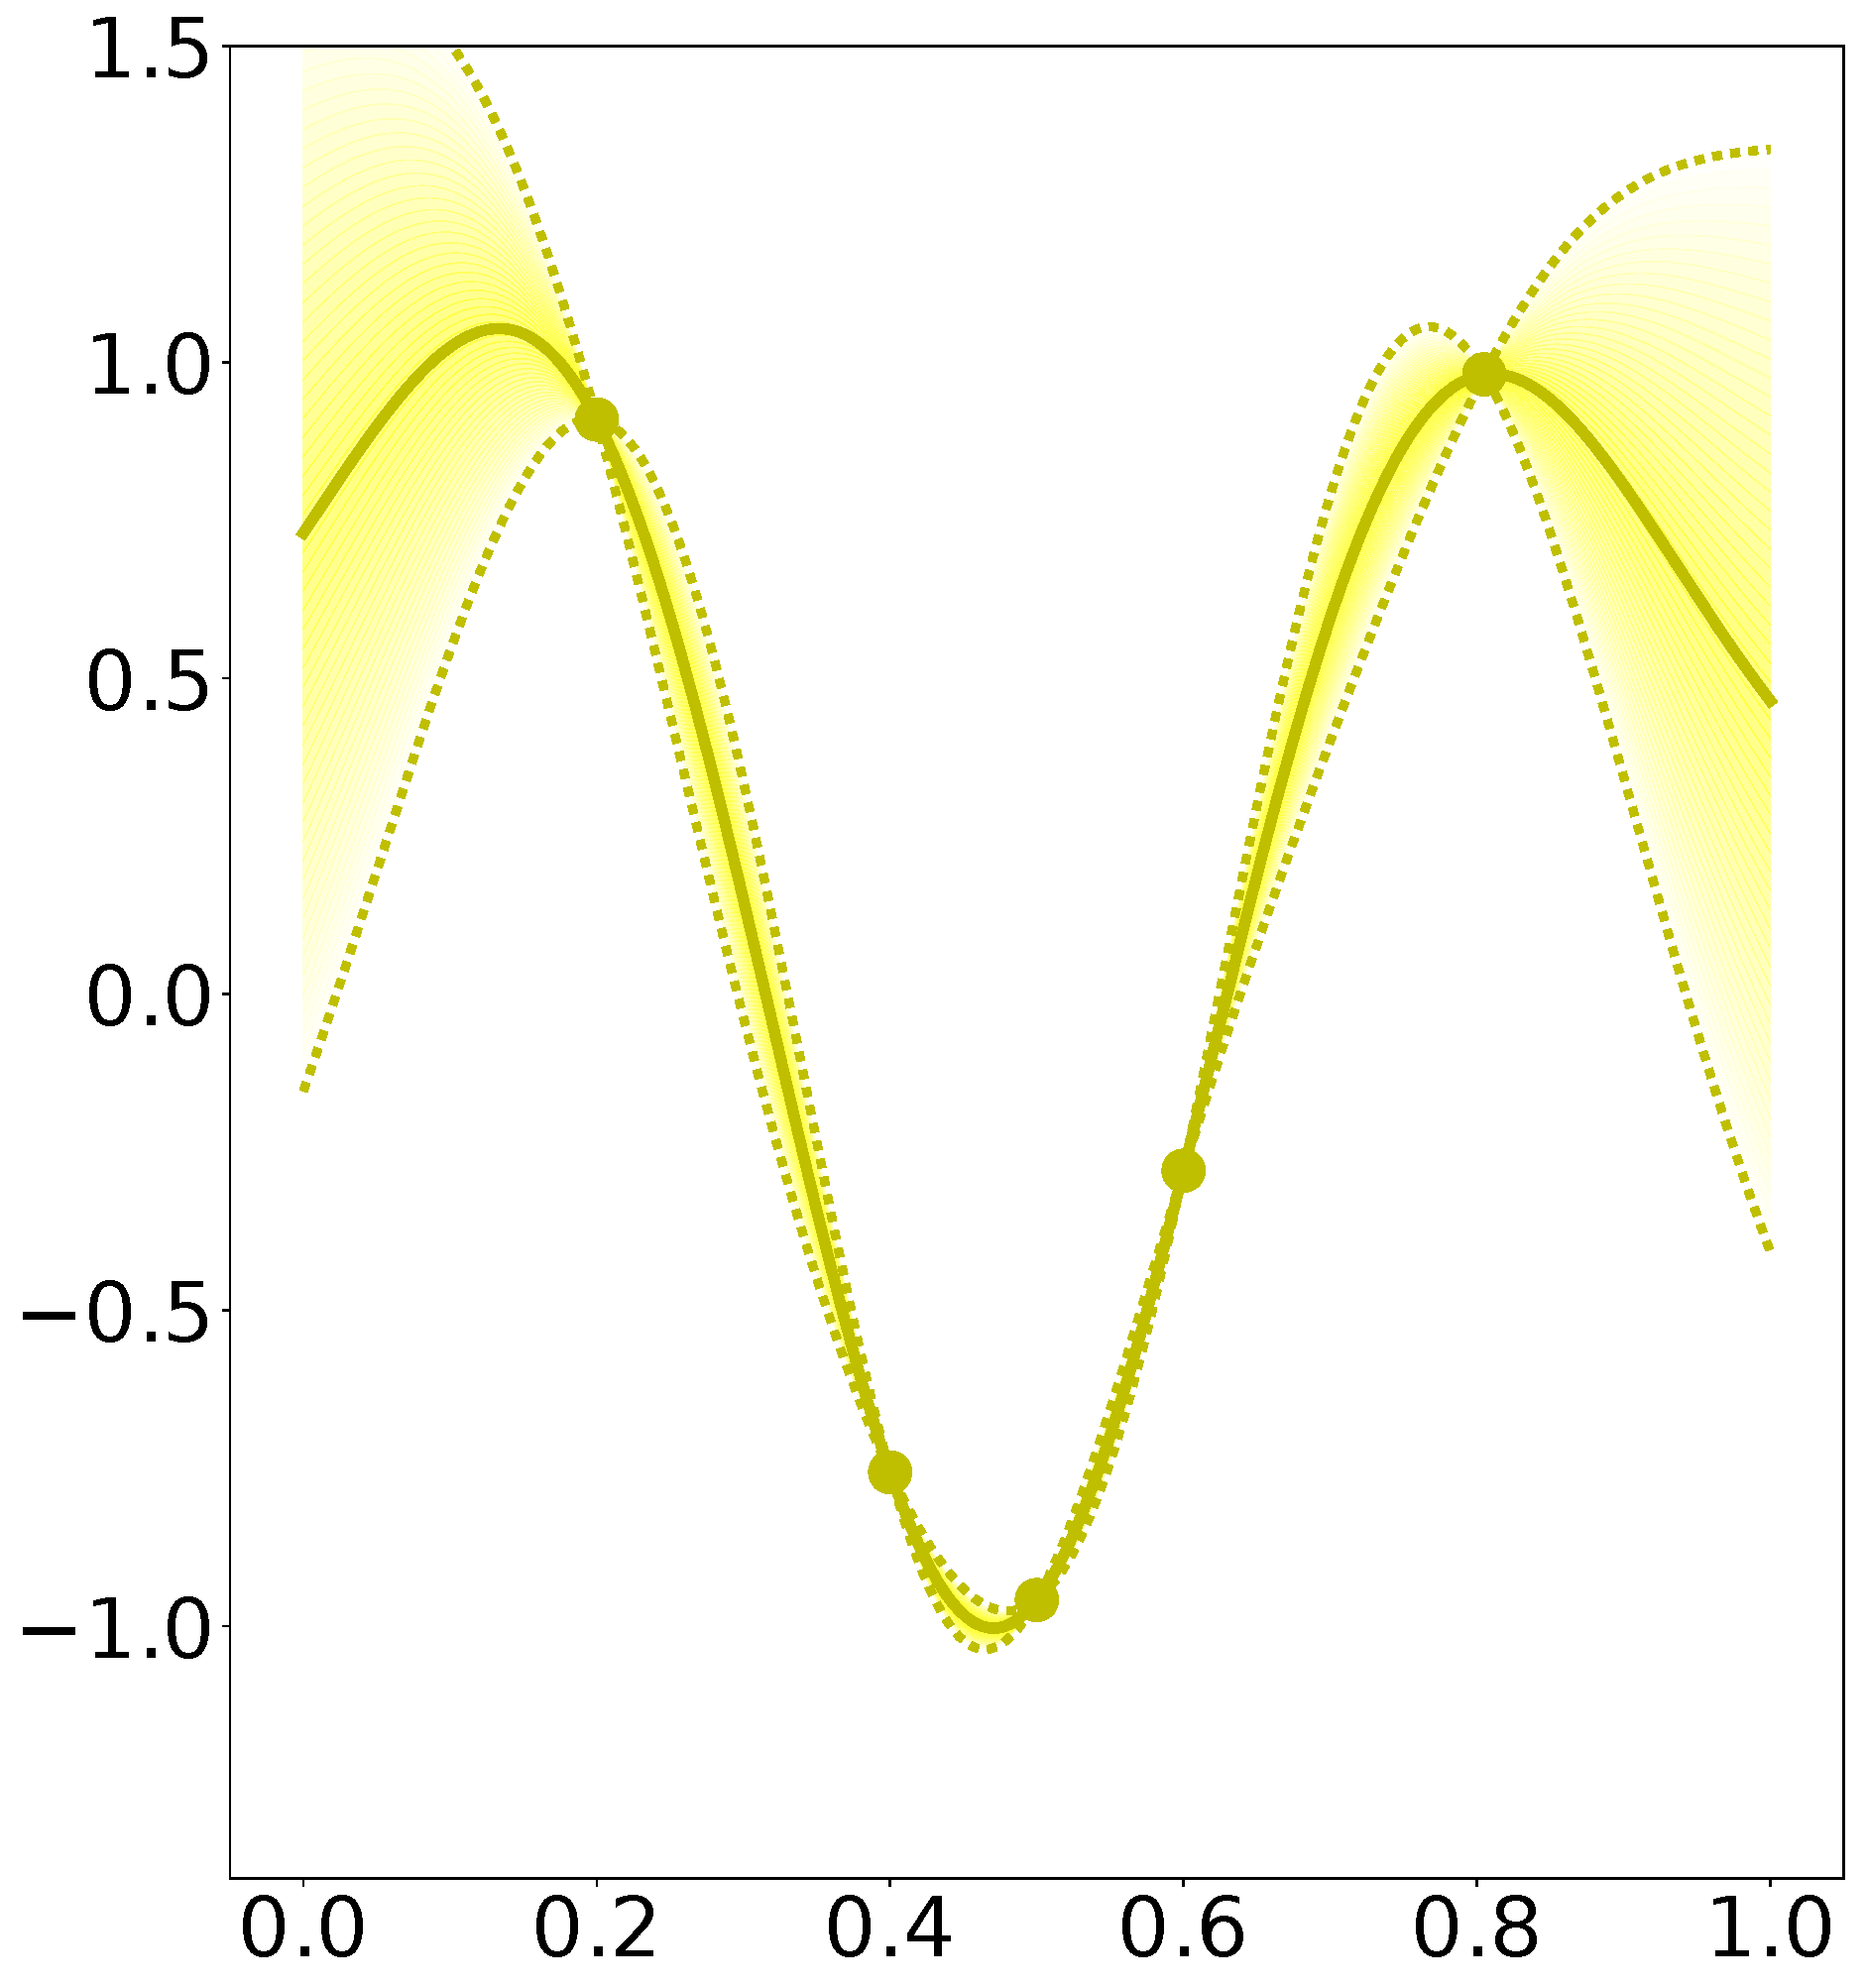
\includegraphics[width=3.4cm,height=3.9cm]{figures/theory/pred1.pdf} & 
        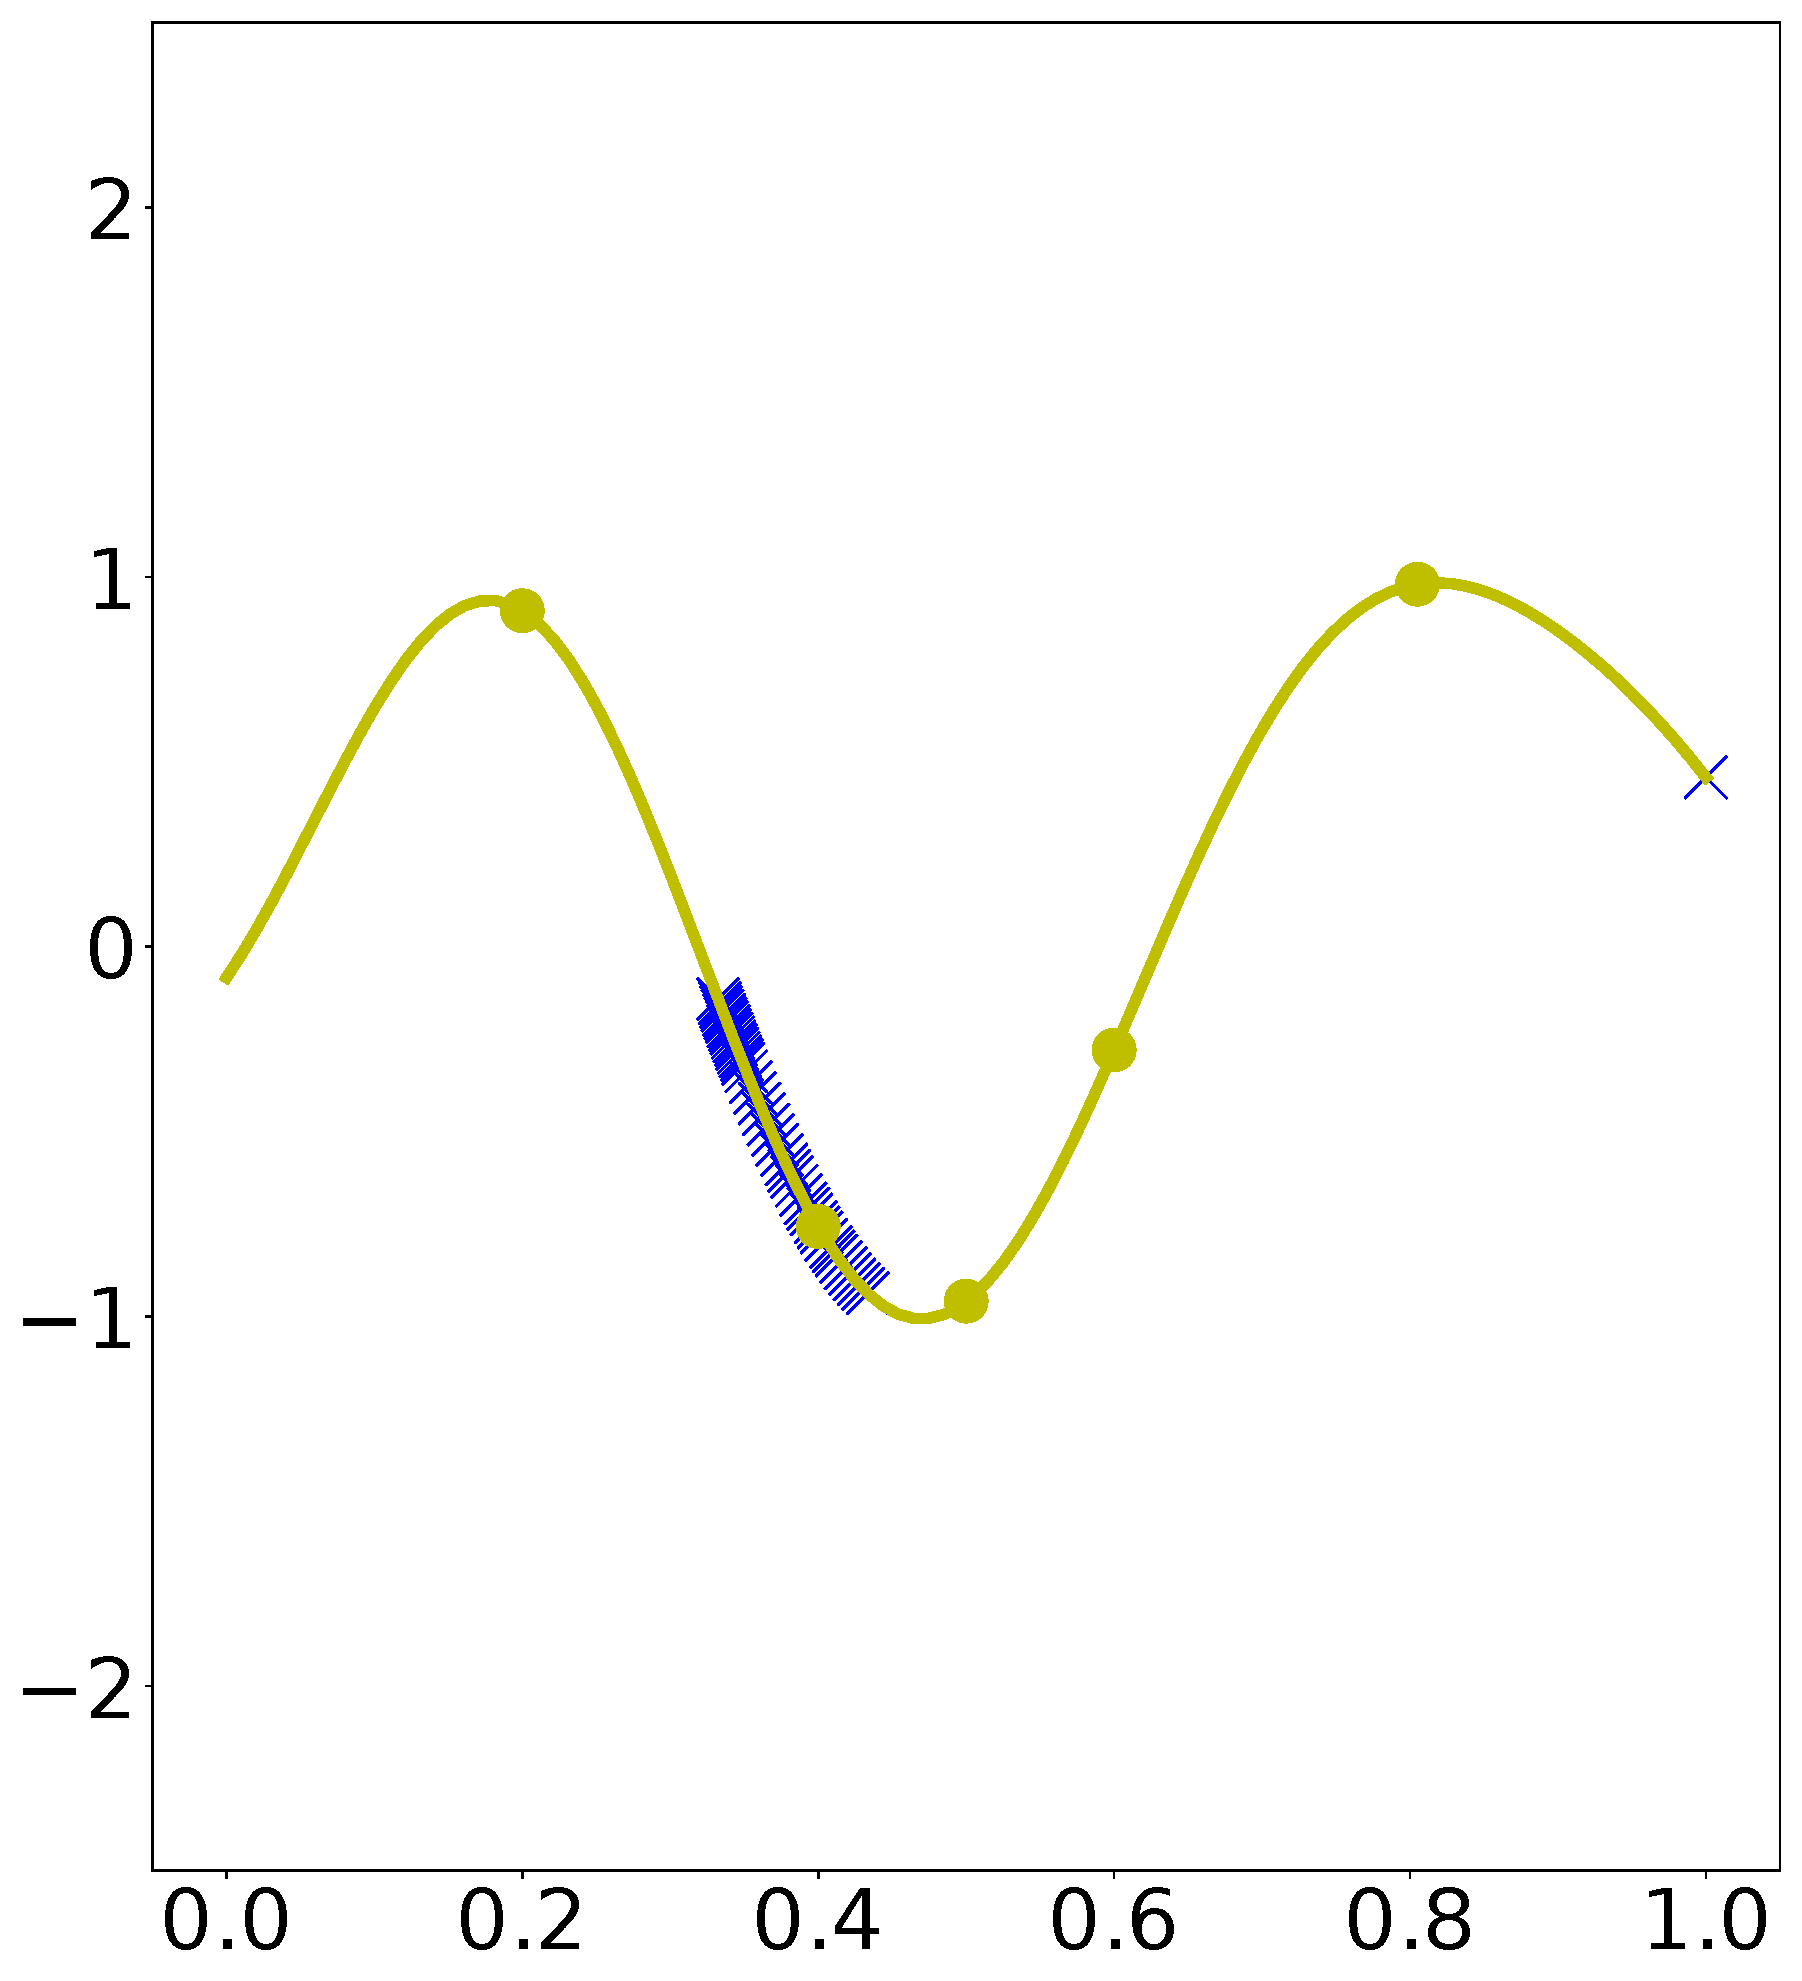
\includegraphics[width=3.4cm,height=3.9cm]{figures/theory/sample1.pdf} & 
	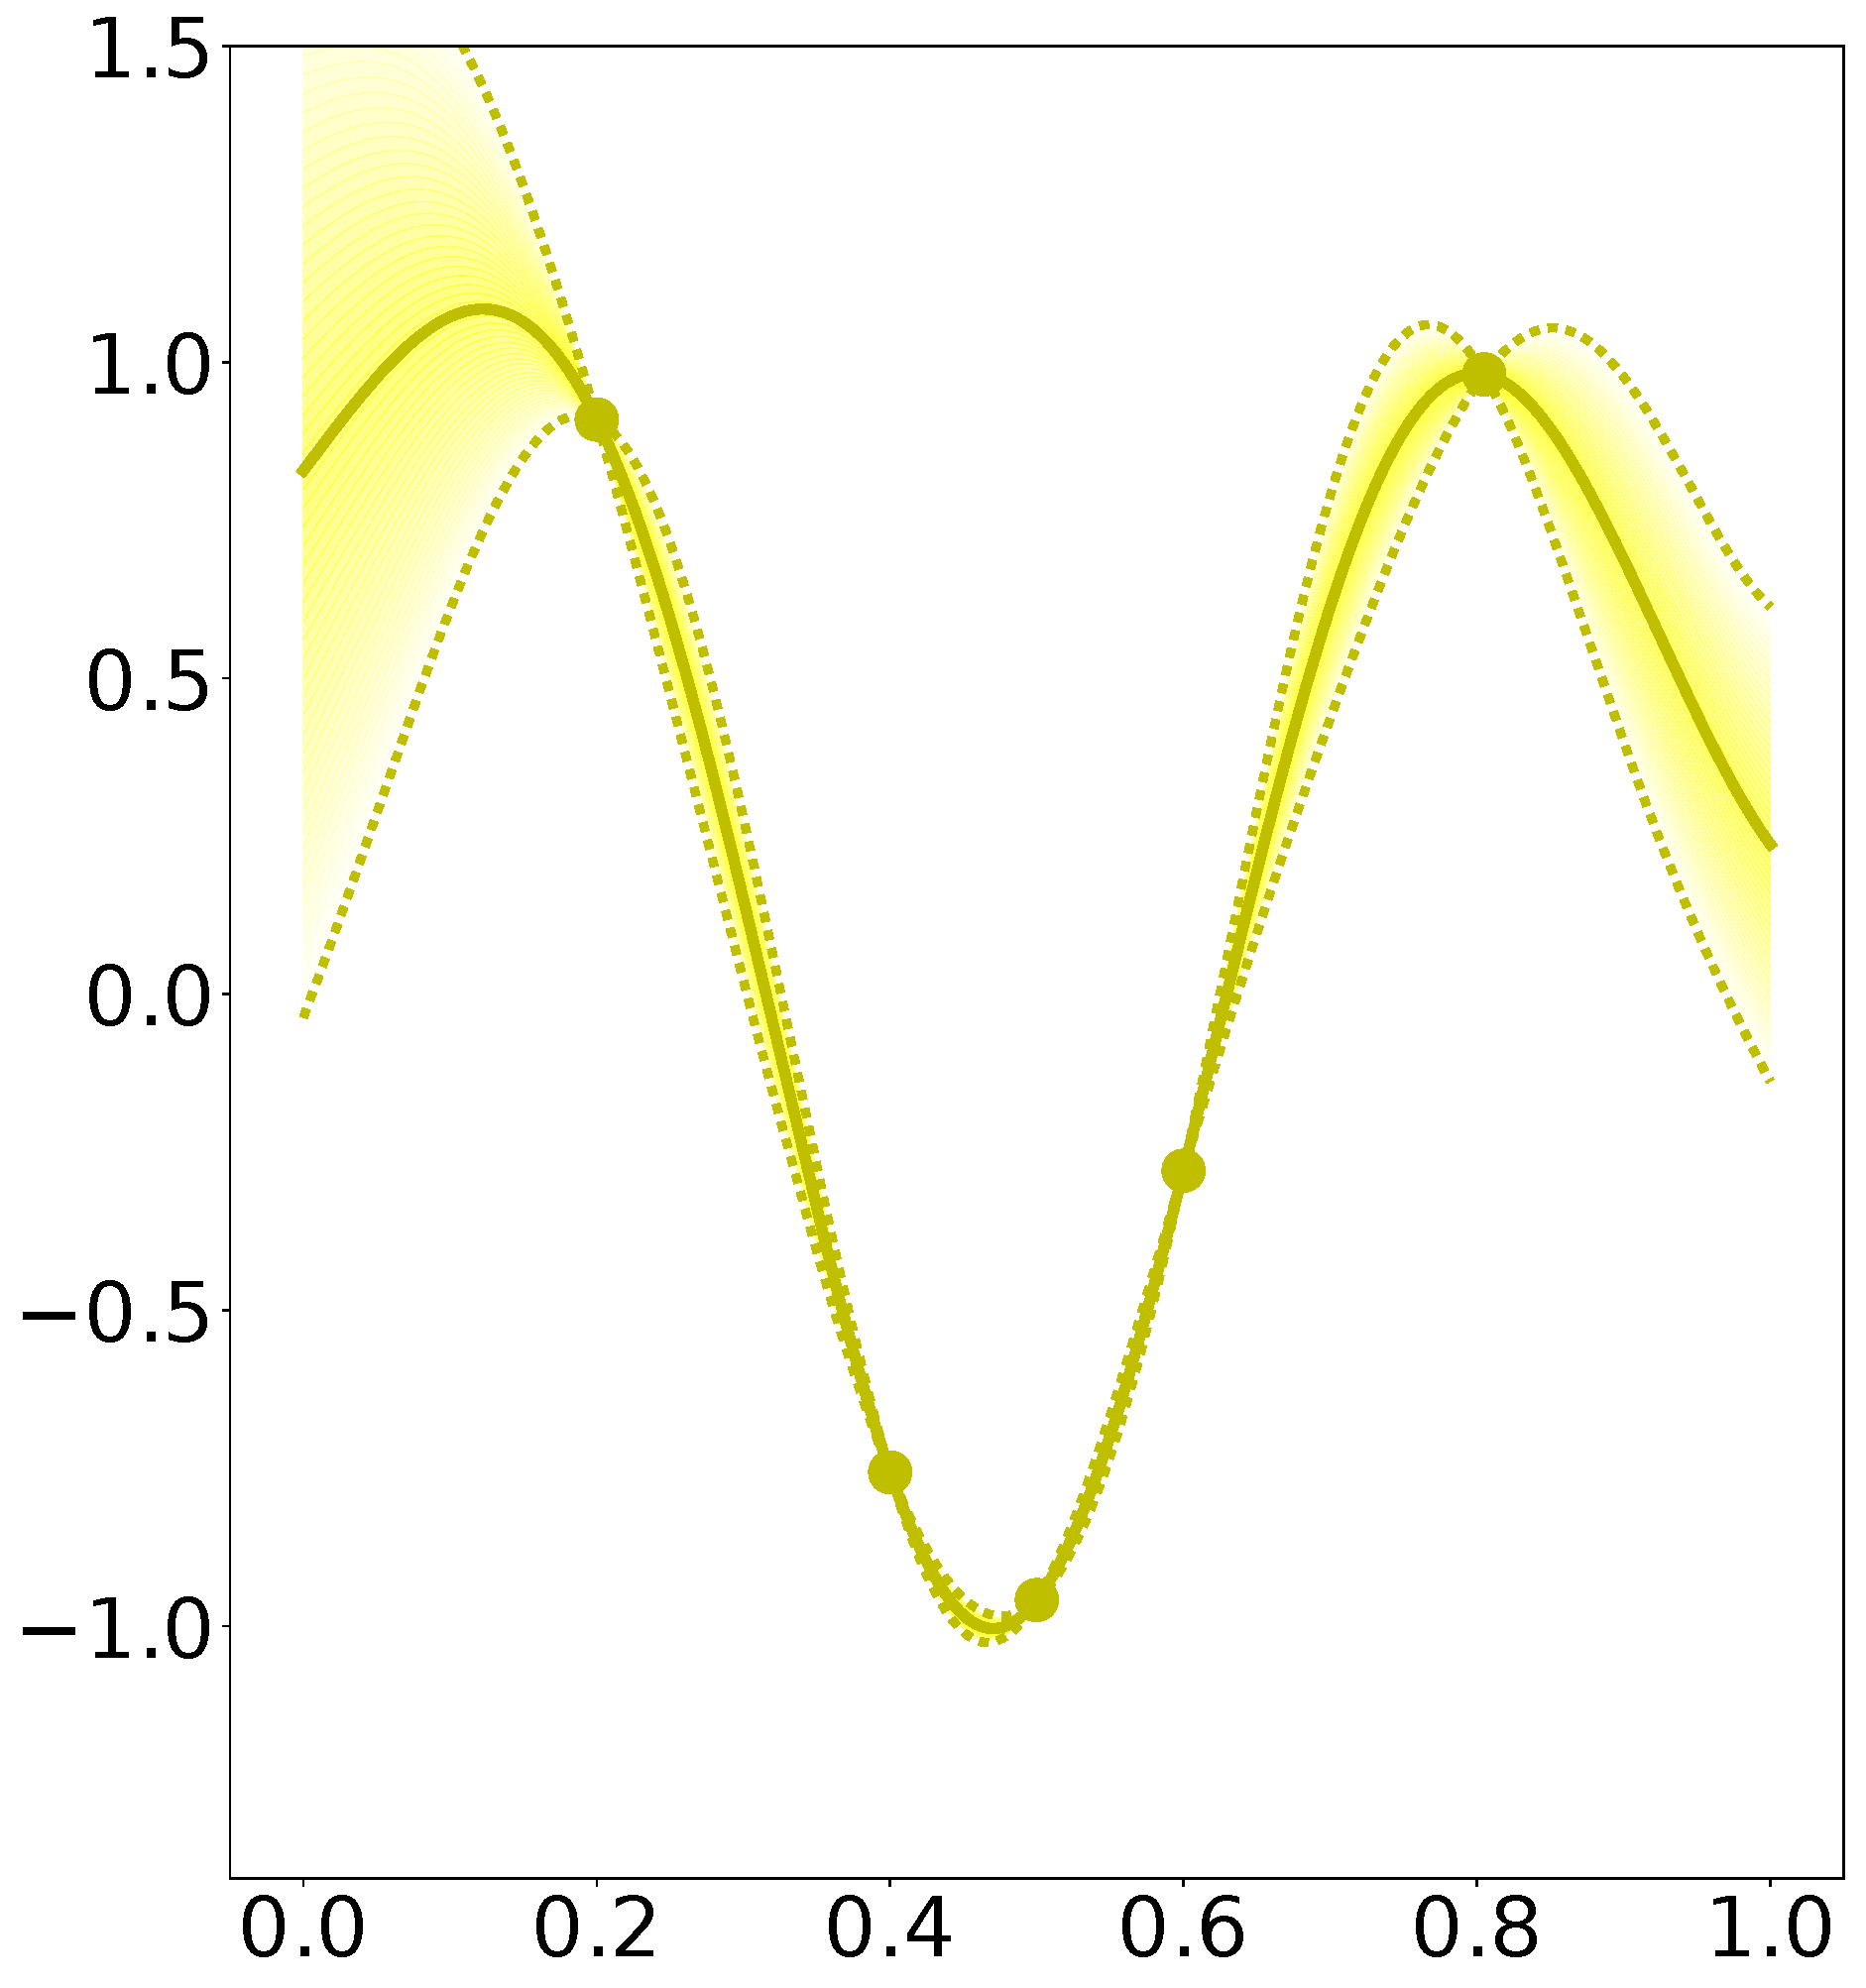
\includegraphics[width=3.4cm,height=3.9cm]{figures/theory/cond_pred1.pdf} & 
        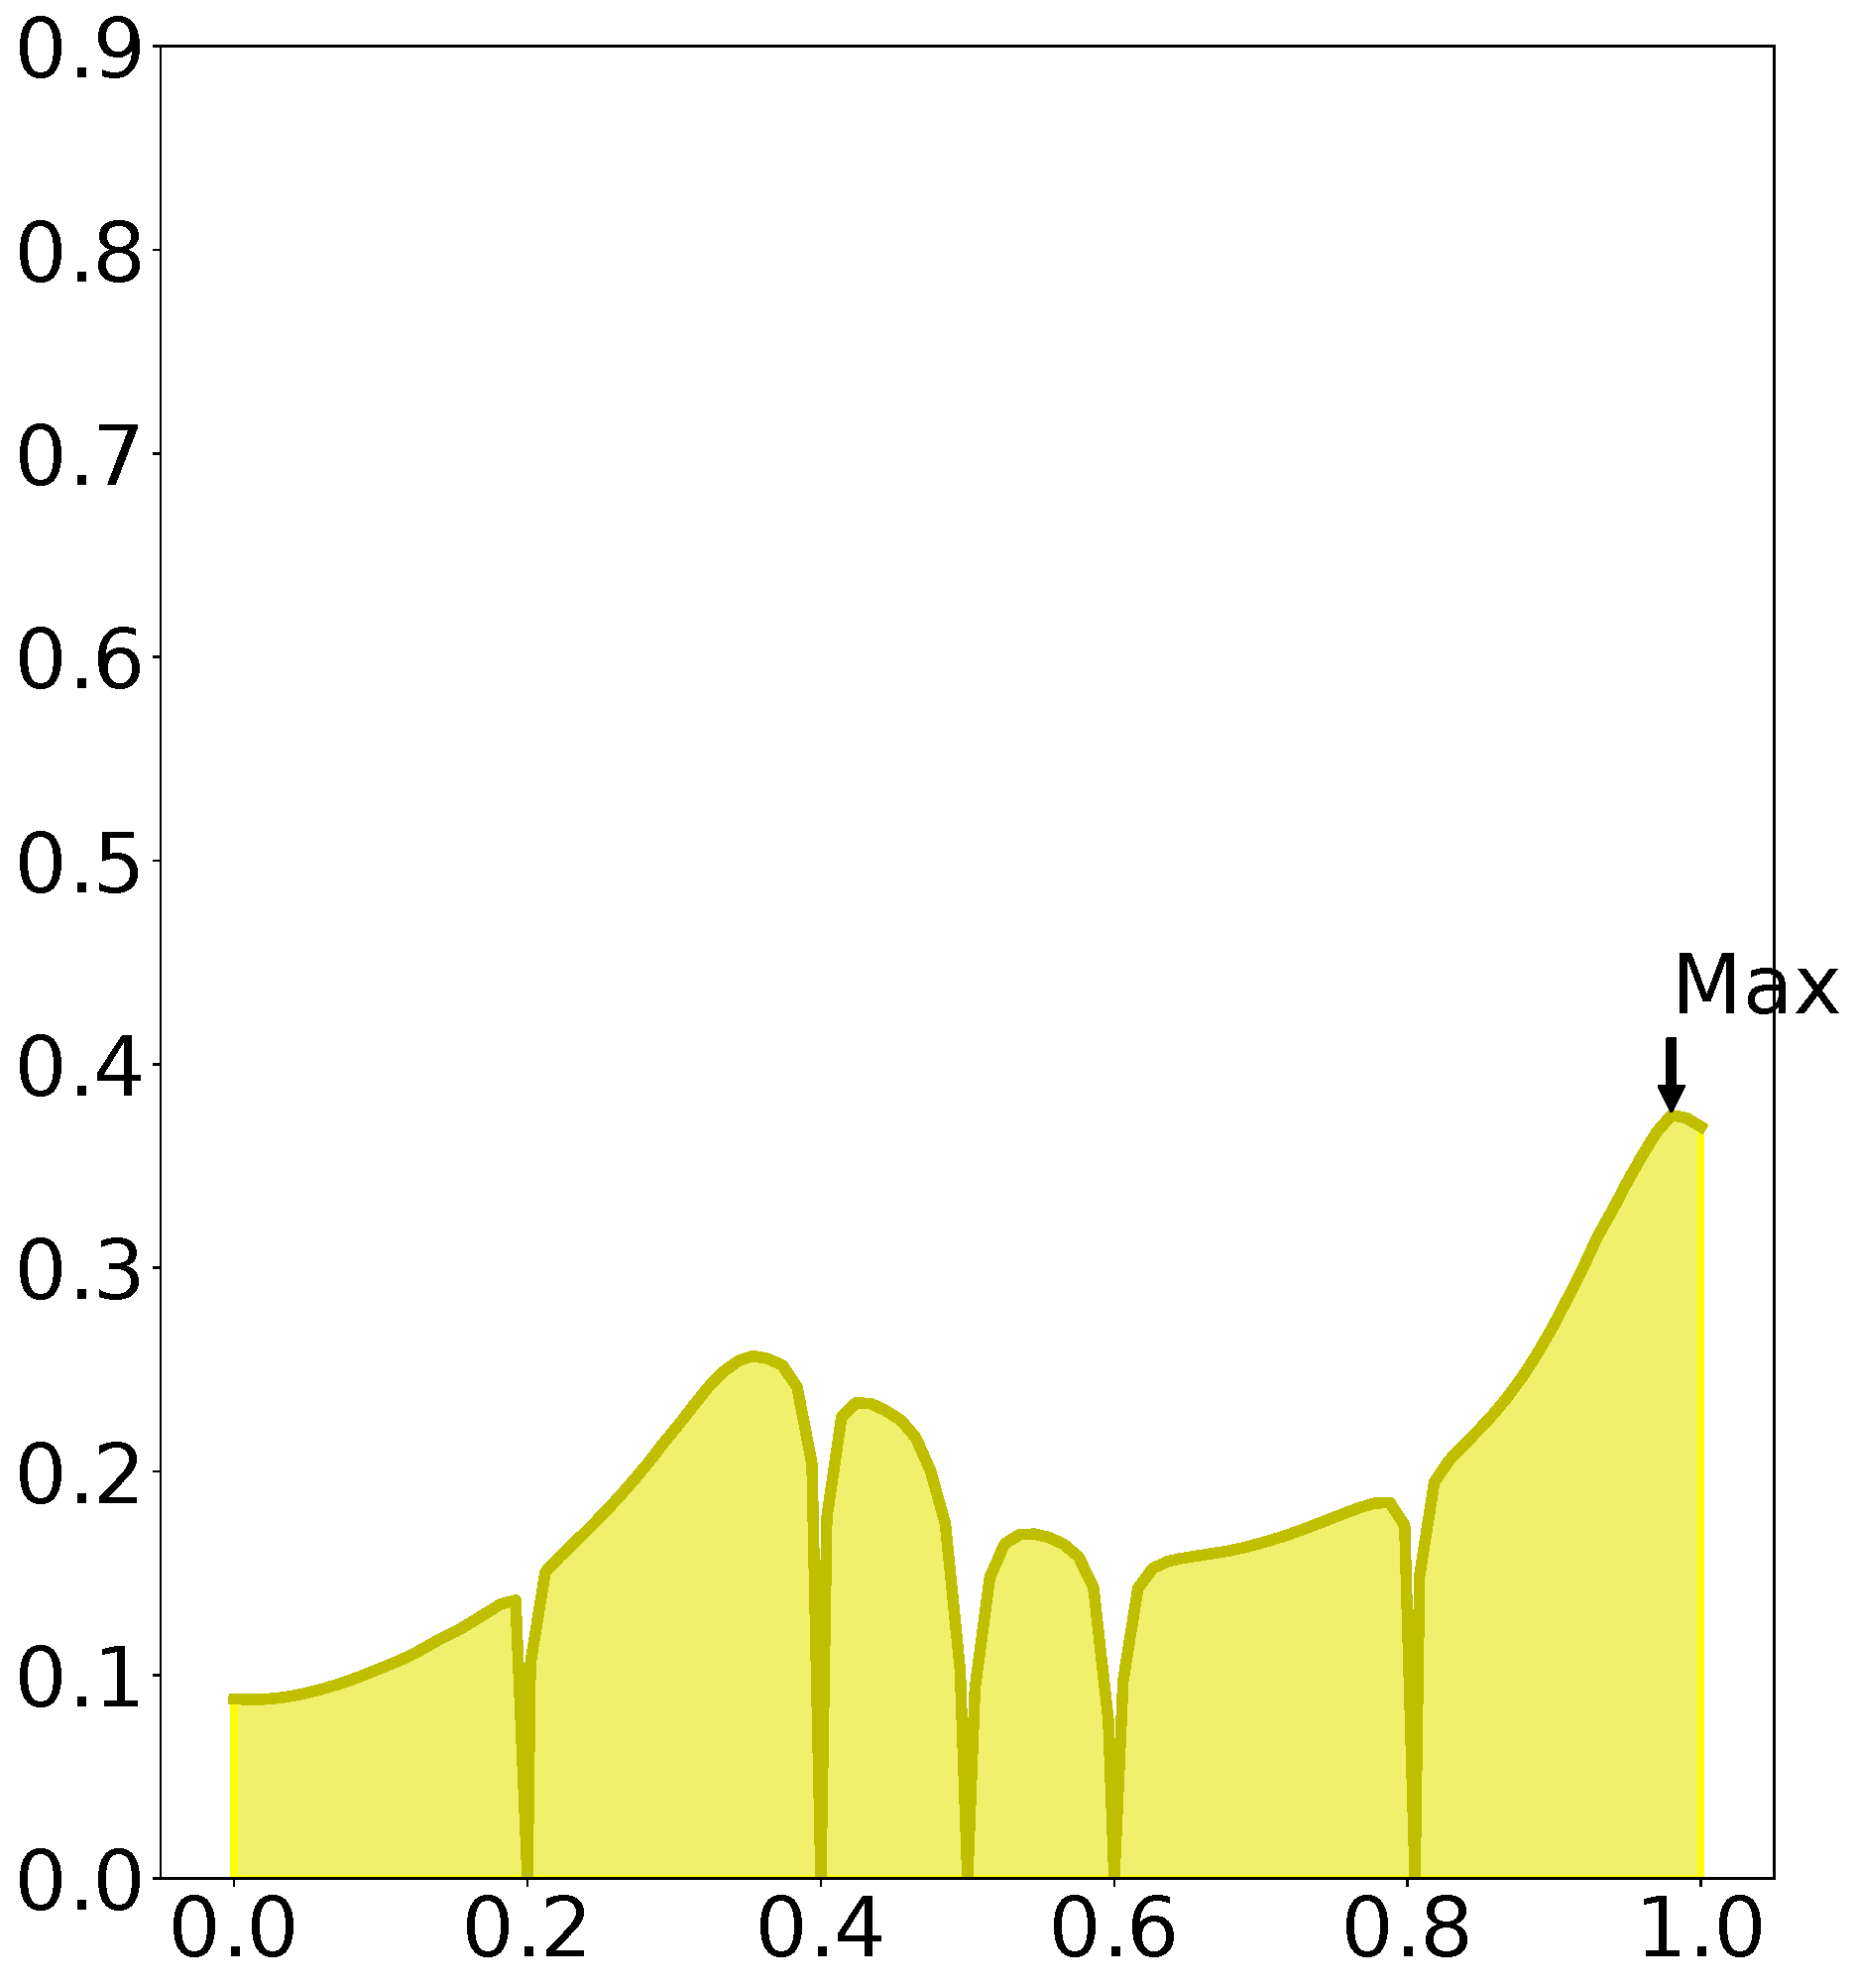
\includegraphics[width=3.4cm,height=3.9cm]{figures/theory/acq1.pdf} \\
	&
	         {{\footnotesize $\mathbf{v}_2^\text{PD}(\mathbf{x})$}}
        &
                {{\footnotesize Sample of $\mathcal{X}^\star$}}
        &
                {{\footnotesize $\mathbf{v}_2^\text{CPD}(\mathbf{x}|\mathcal{X}^\star_1)$}}
        &
                {{\footnotesize $\alpha_2^\text{obj}(\mathbf{x})$}} \\

	\rotatebox{90}{\hspace{1.5cm}$f_2(\mathbf{x})$} &
	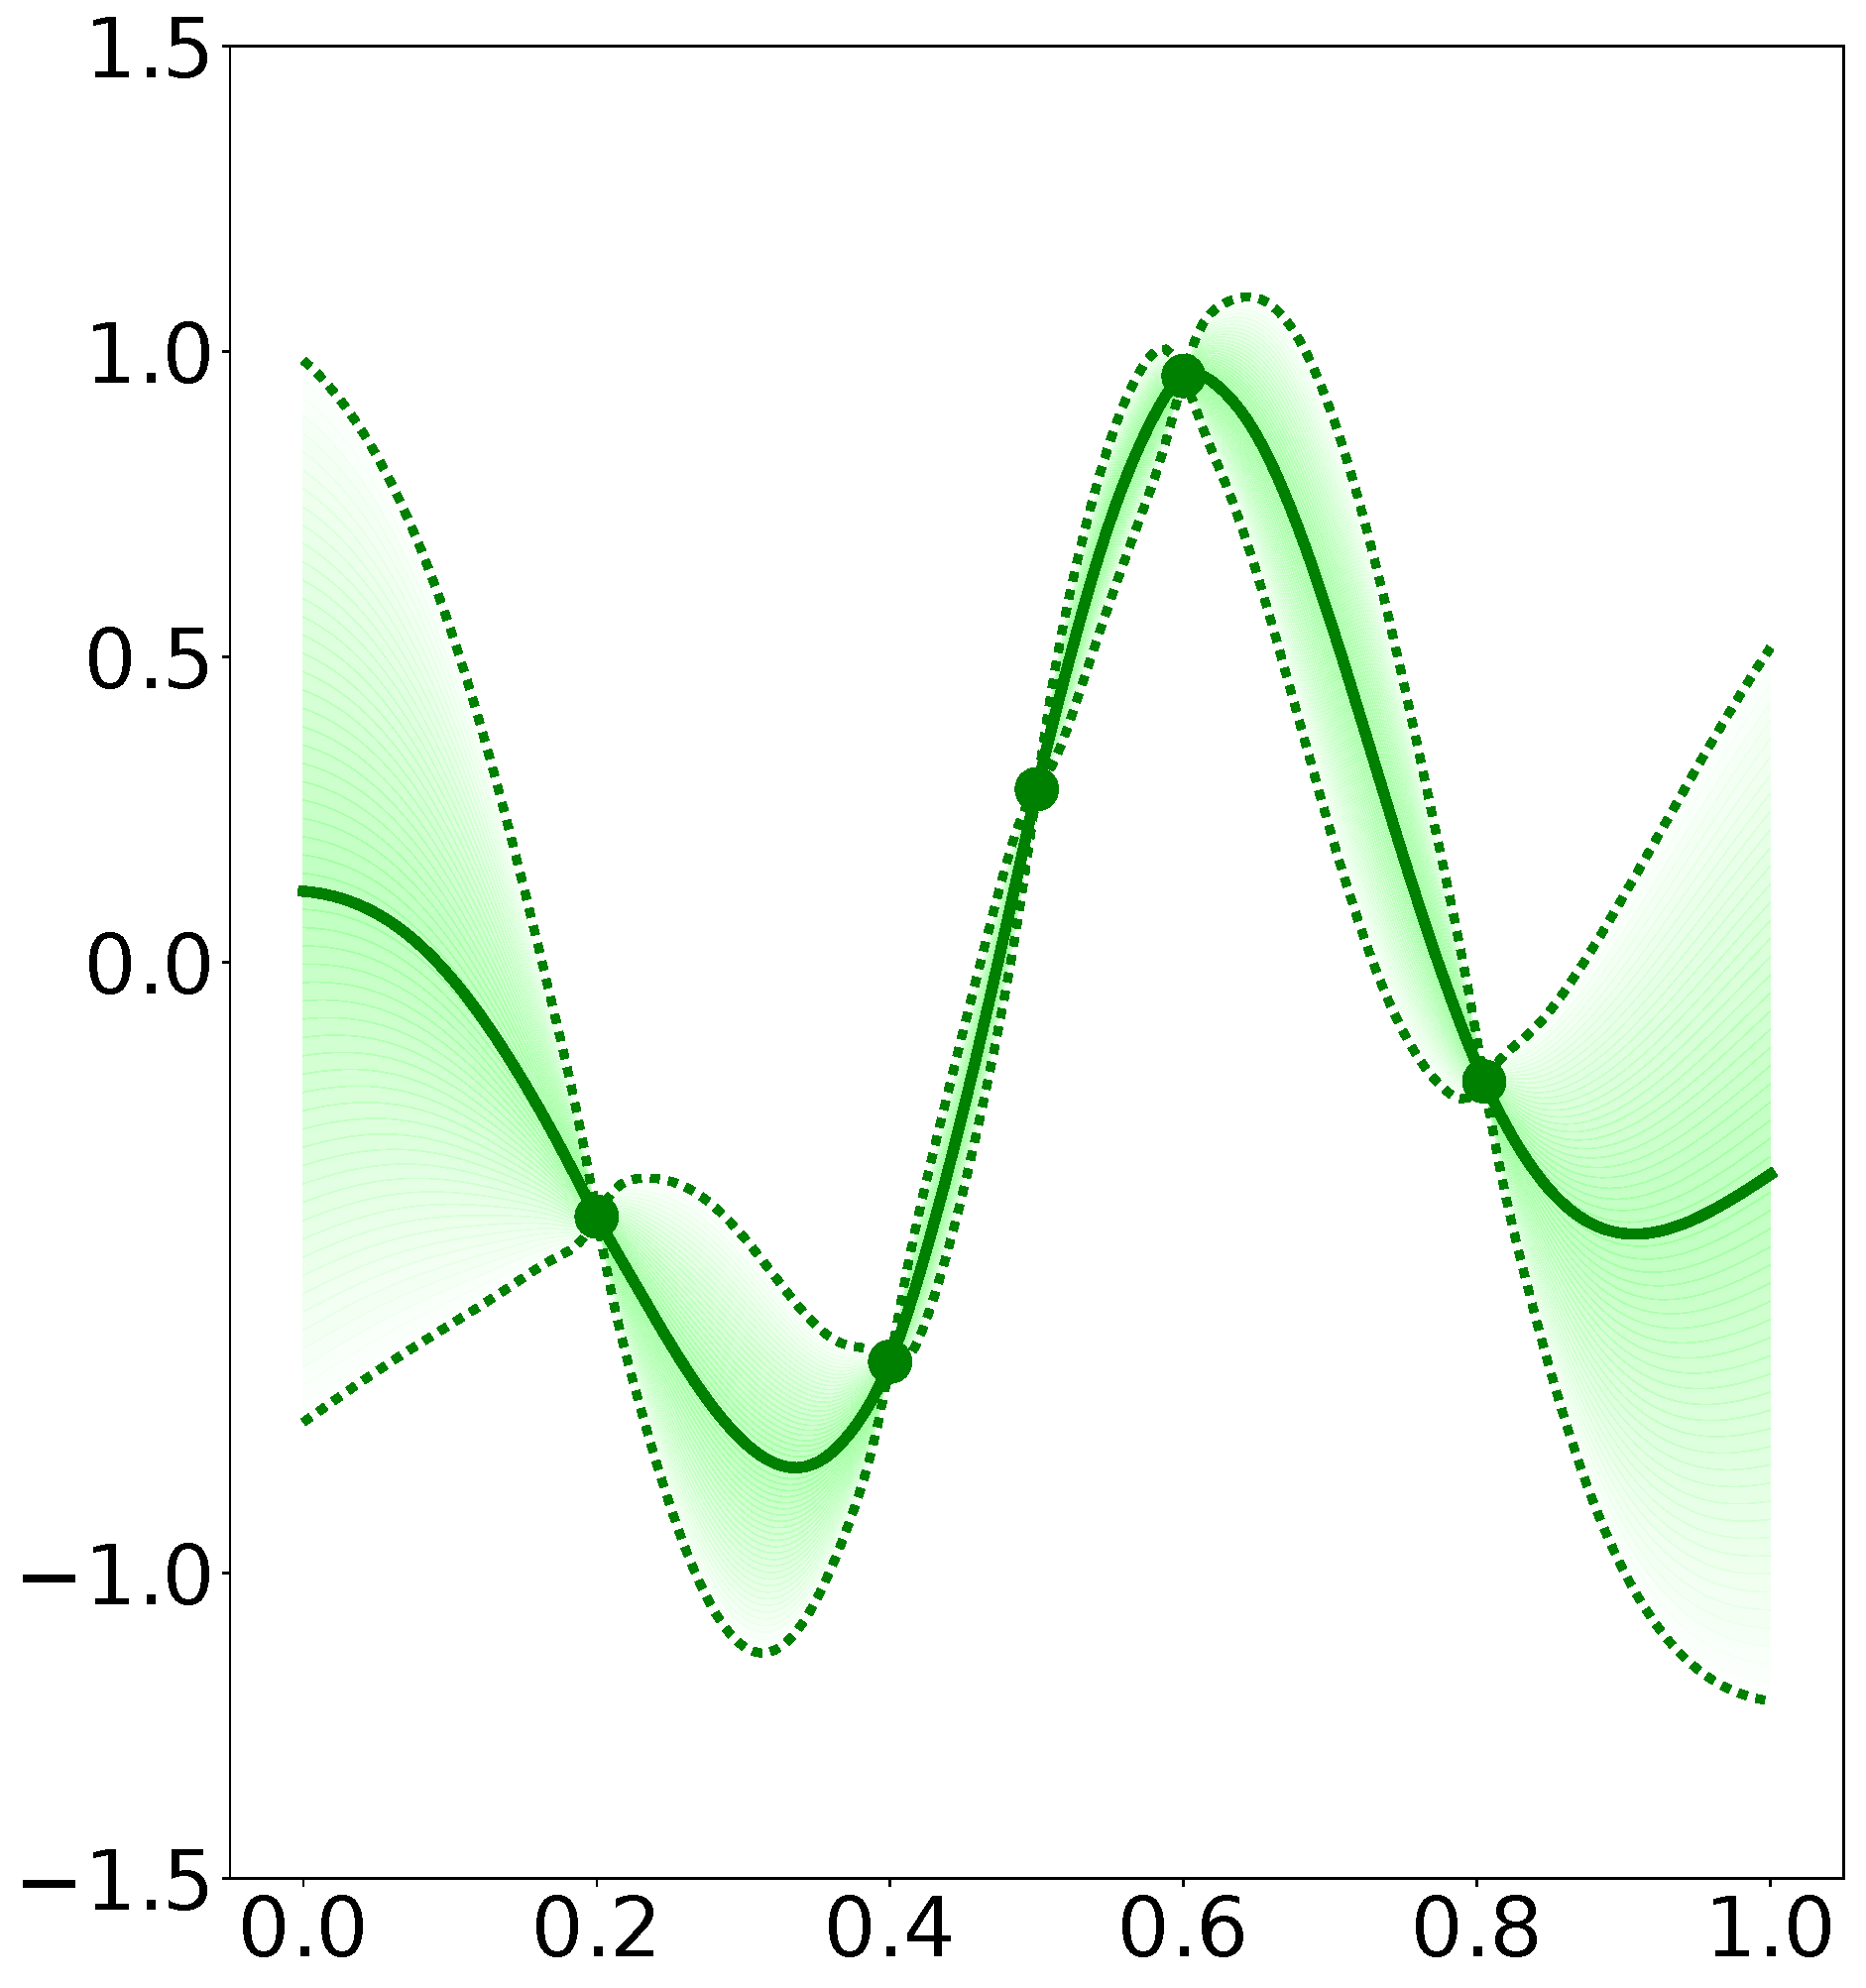
\includegraphics[width=3.4cm,,height=3.9cm]{figures/theory/pred2.pdf} &
        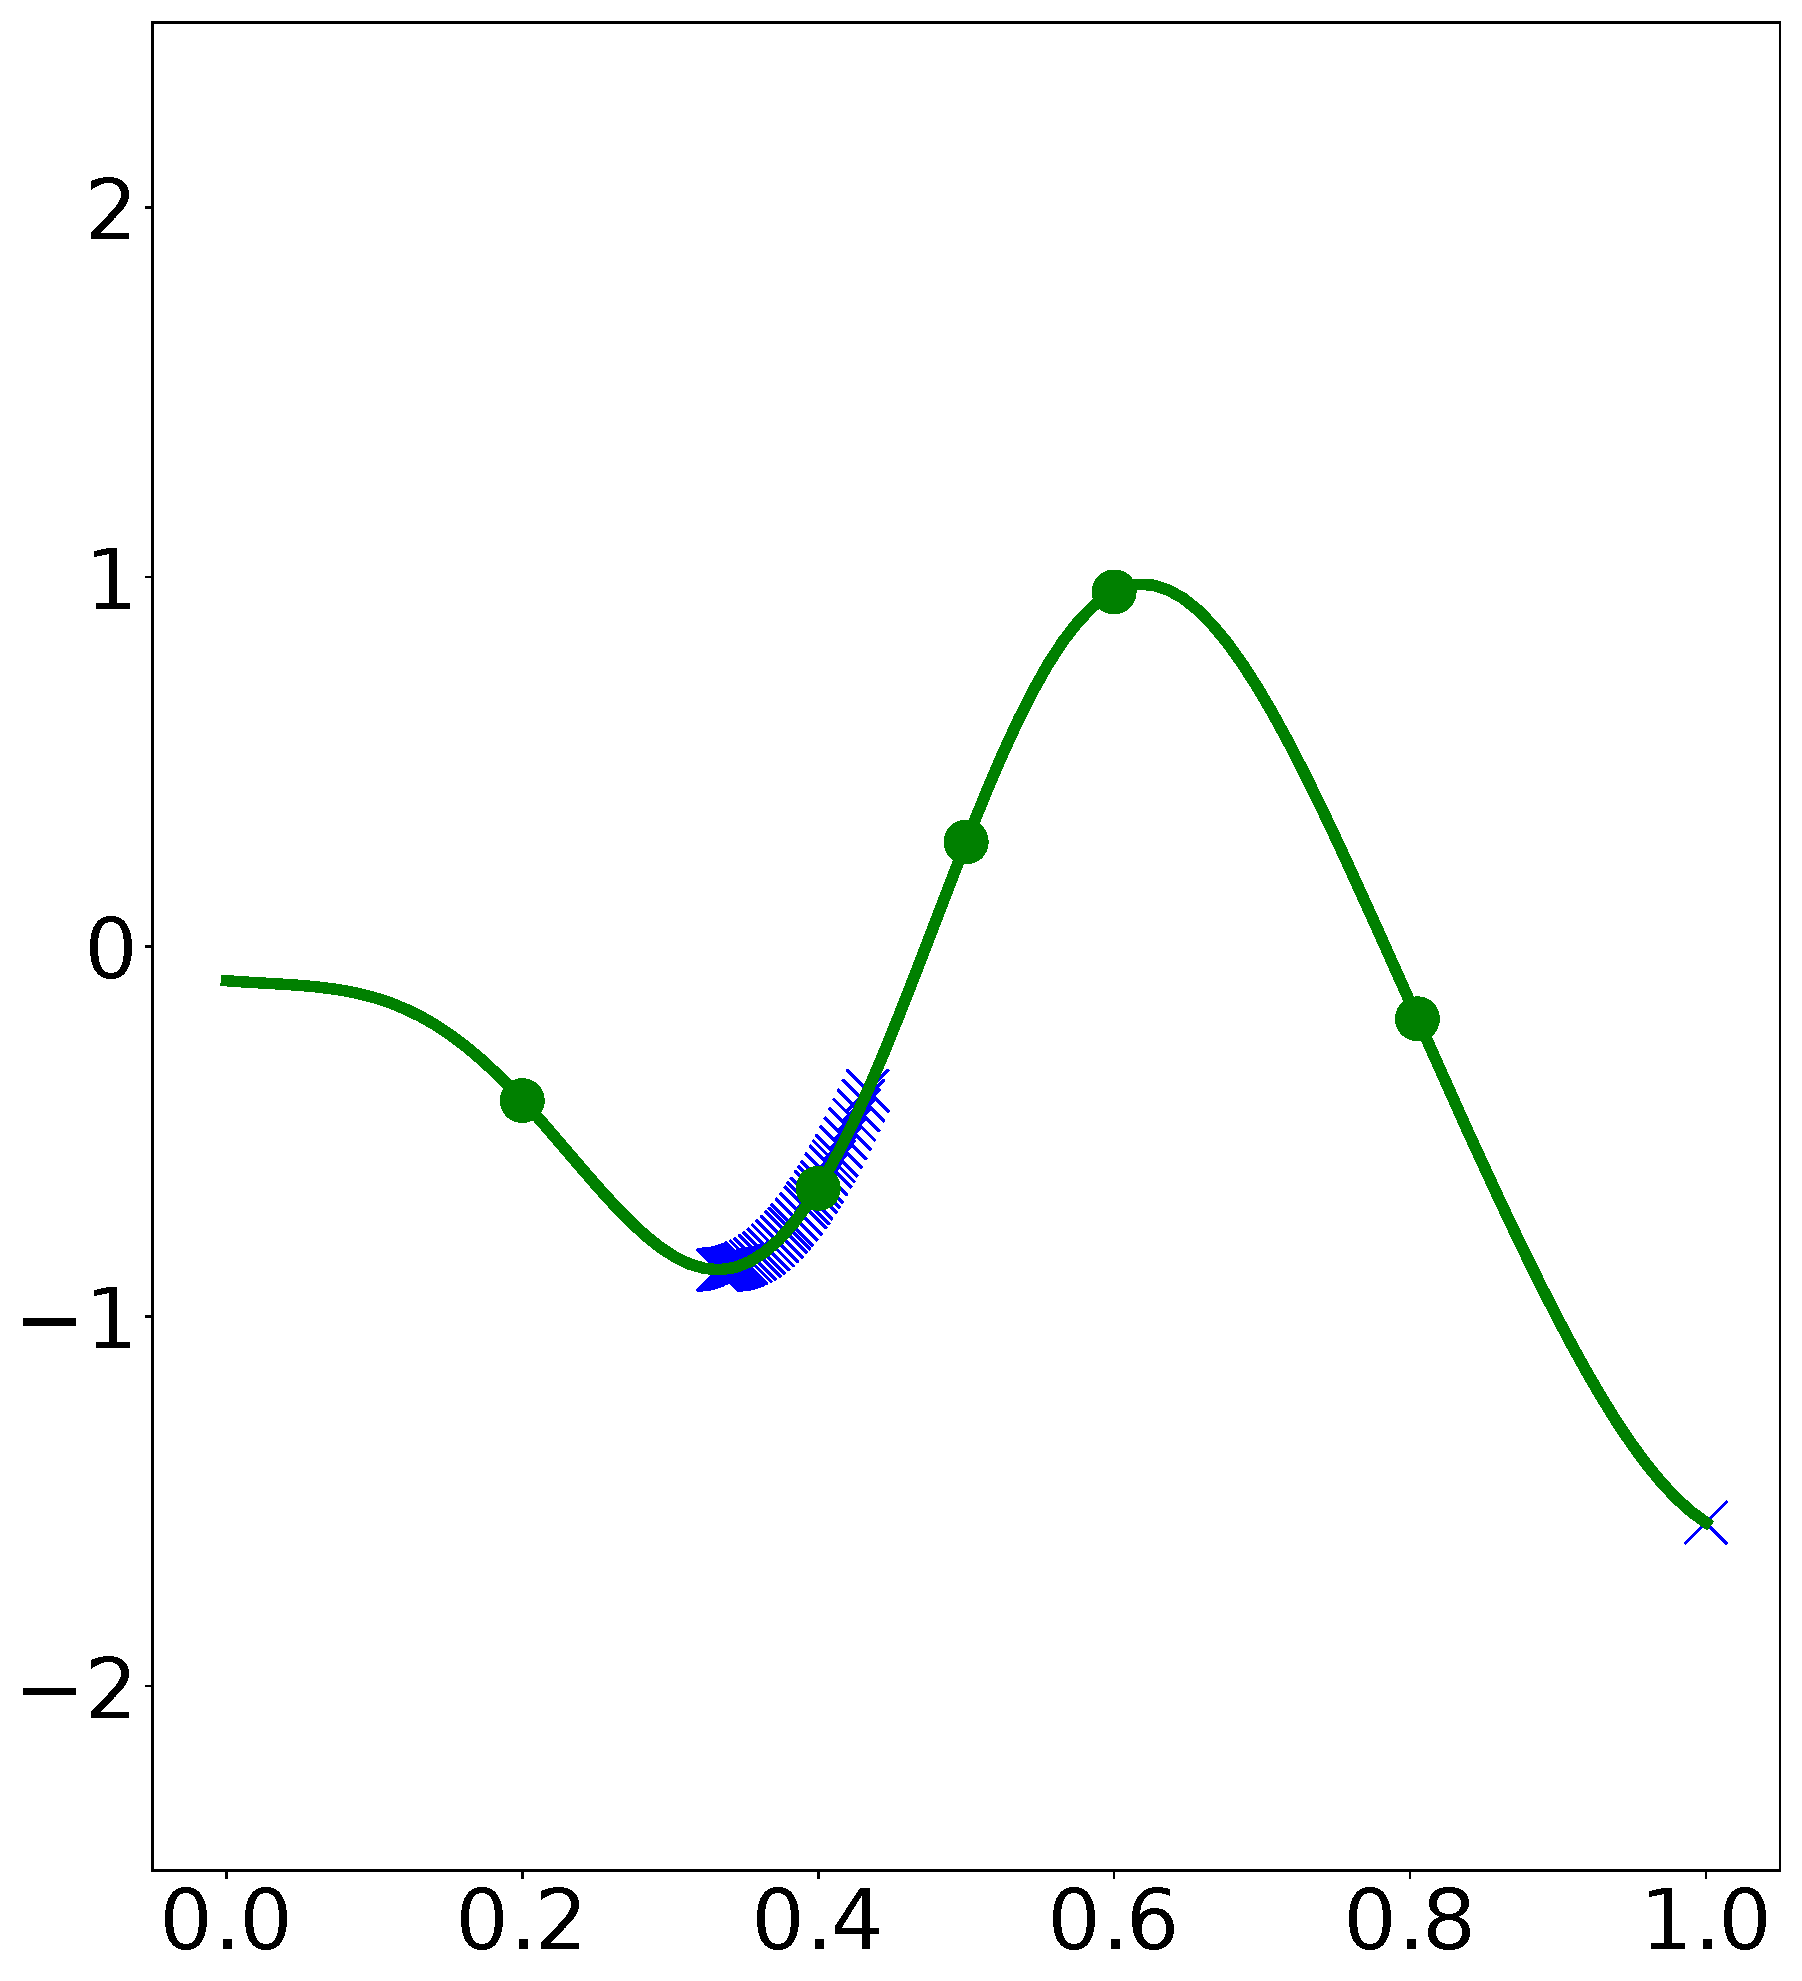
\includegraphics[width=3.4cm,,height=3.9cm]{figures/theory/sample2.pdf} & 
	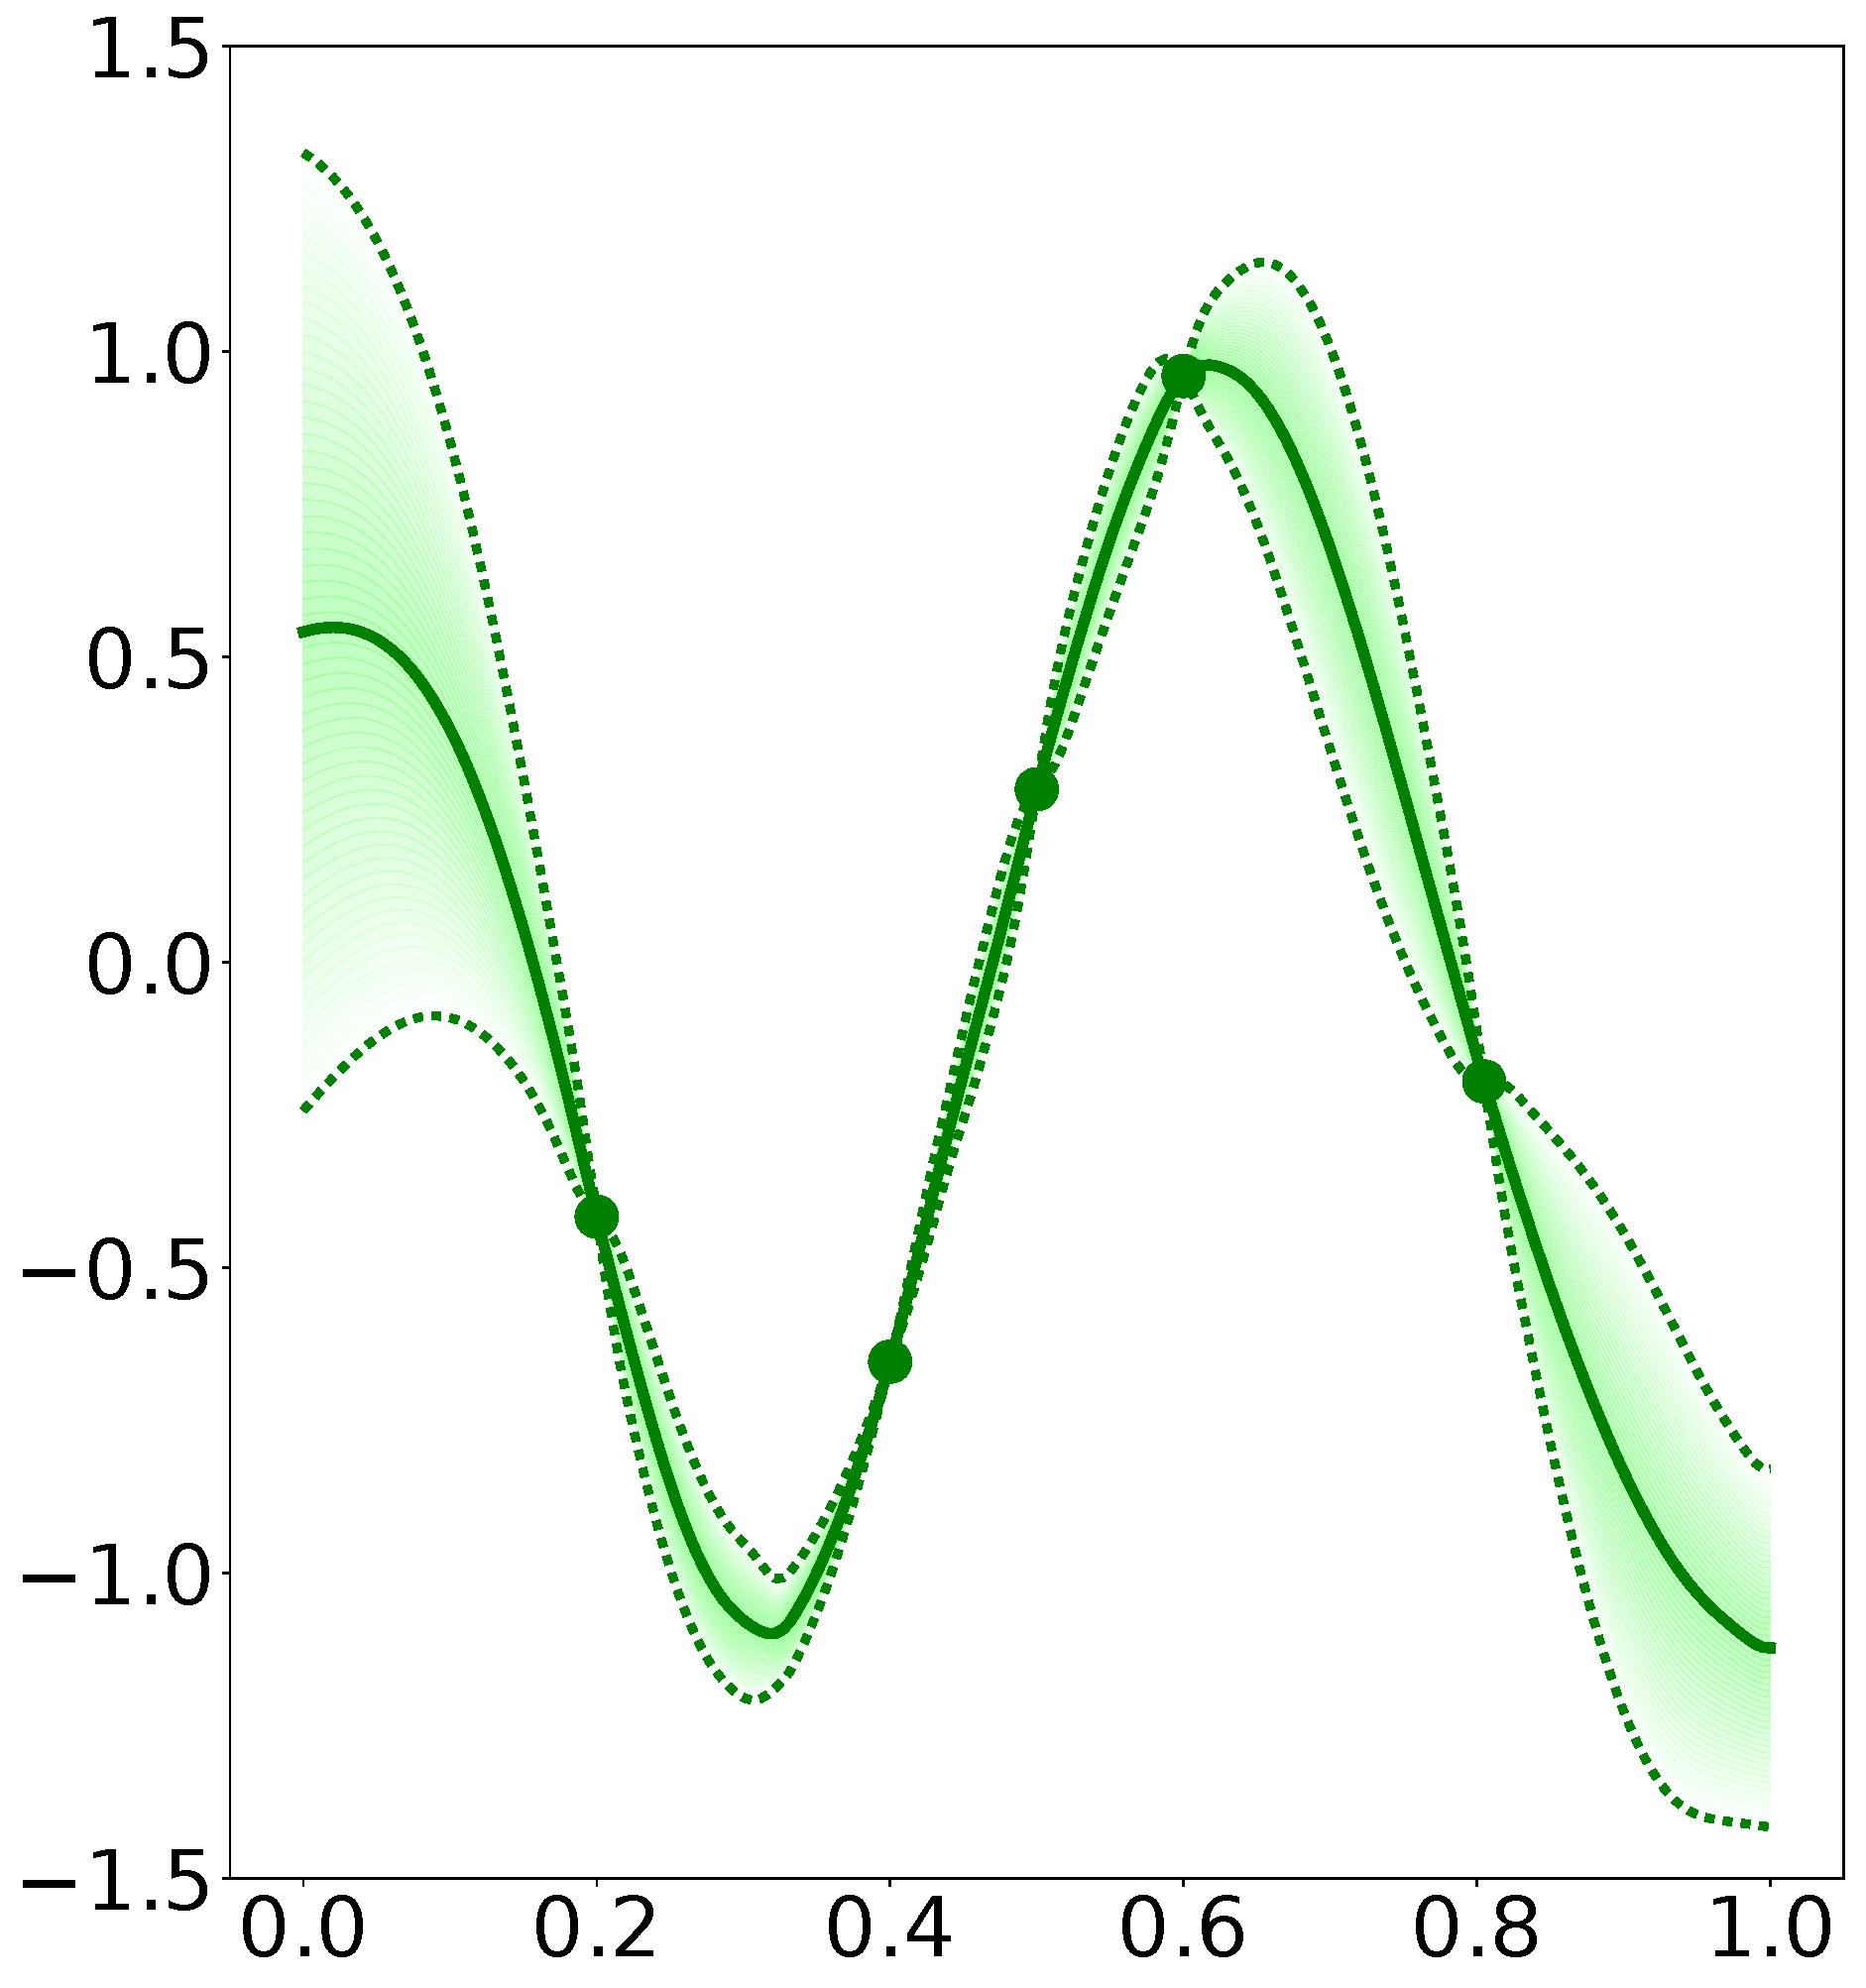
\includegraphics[width=3.4cm,,height=3.9cm]{figures/theory/cond_pred2.pdf} & 
        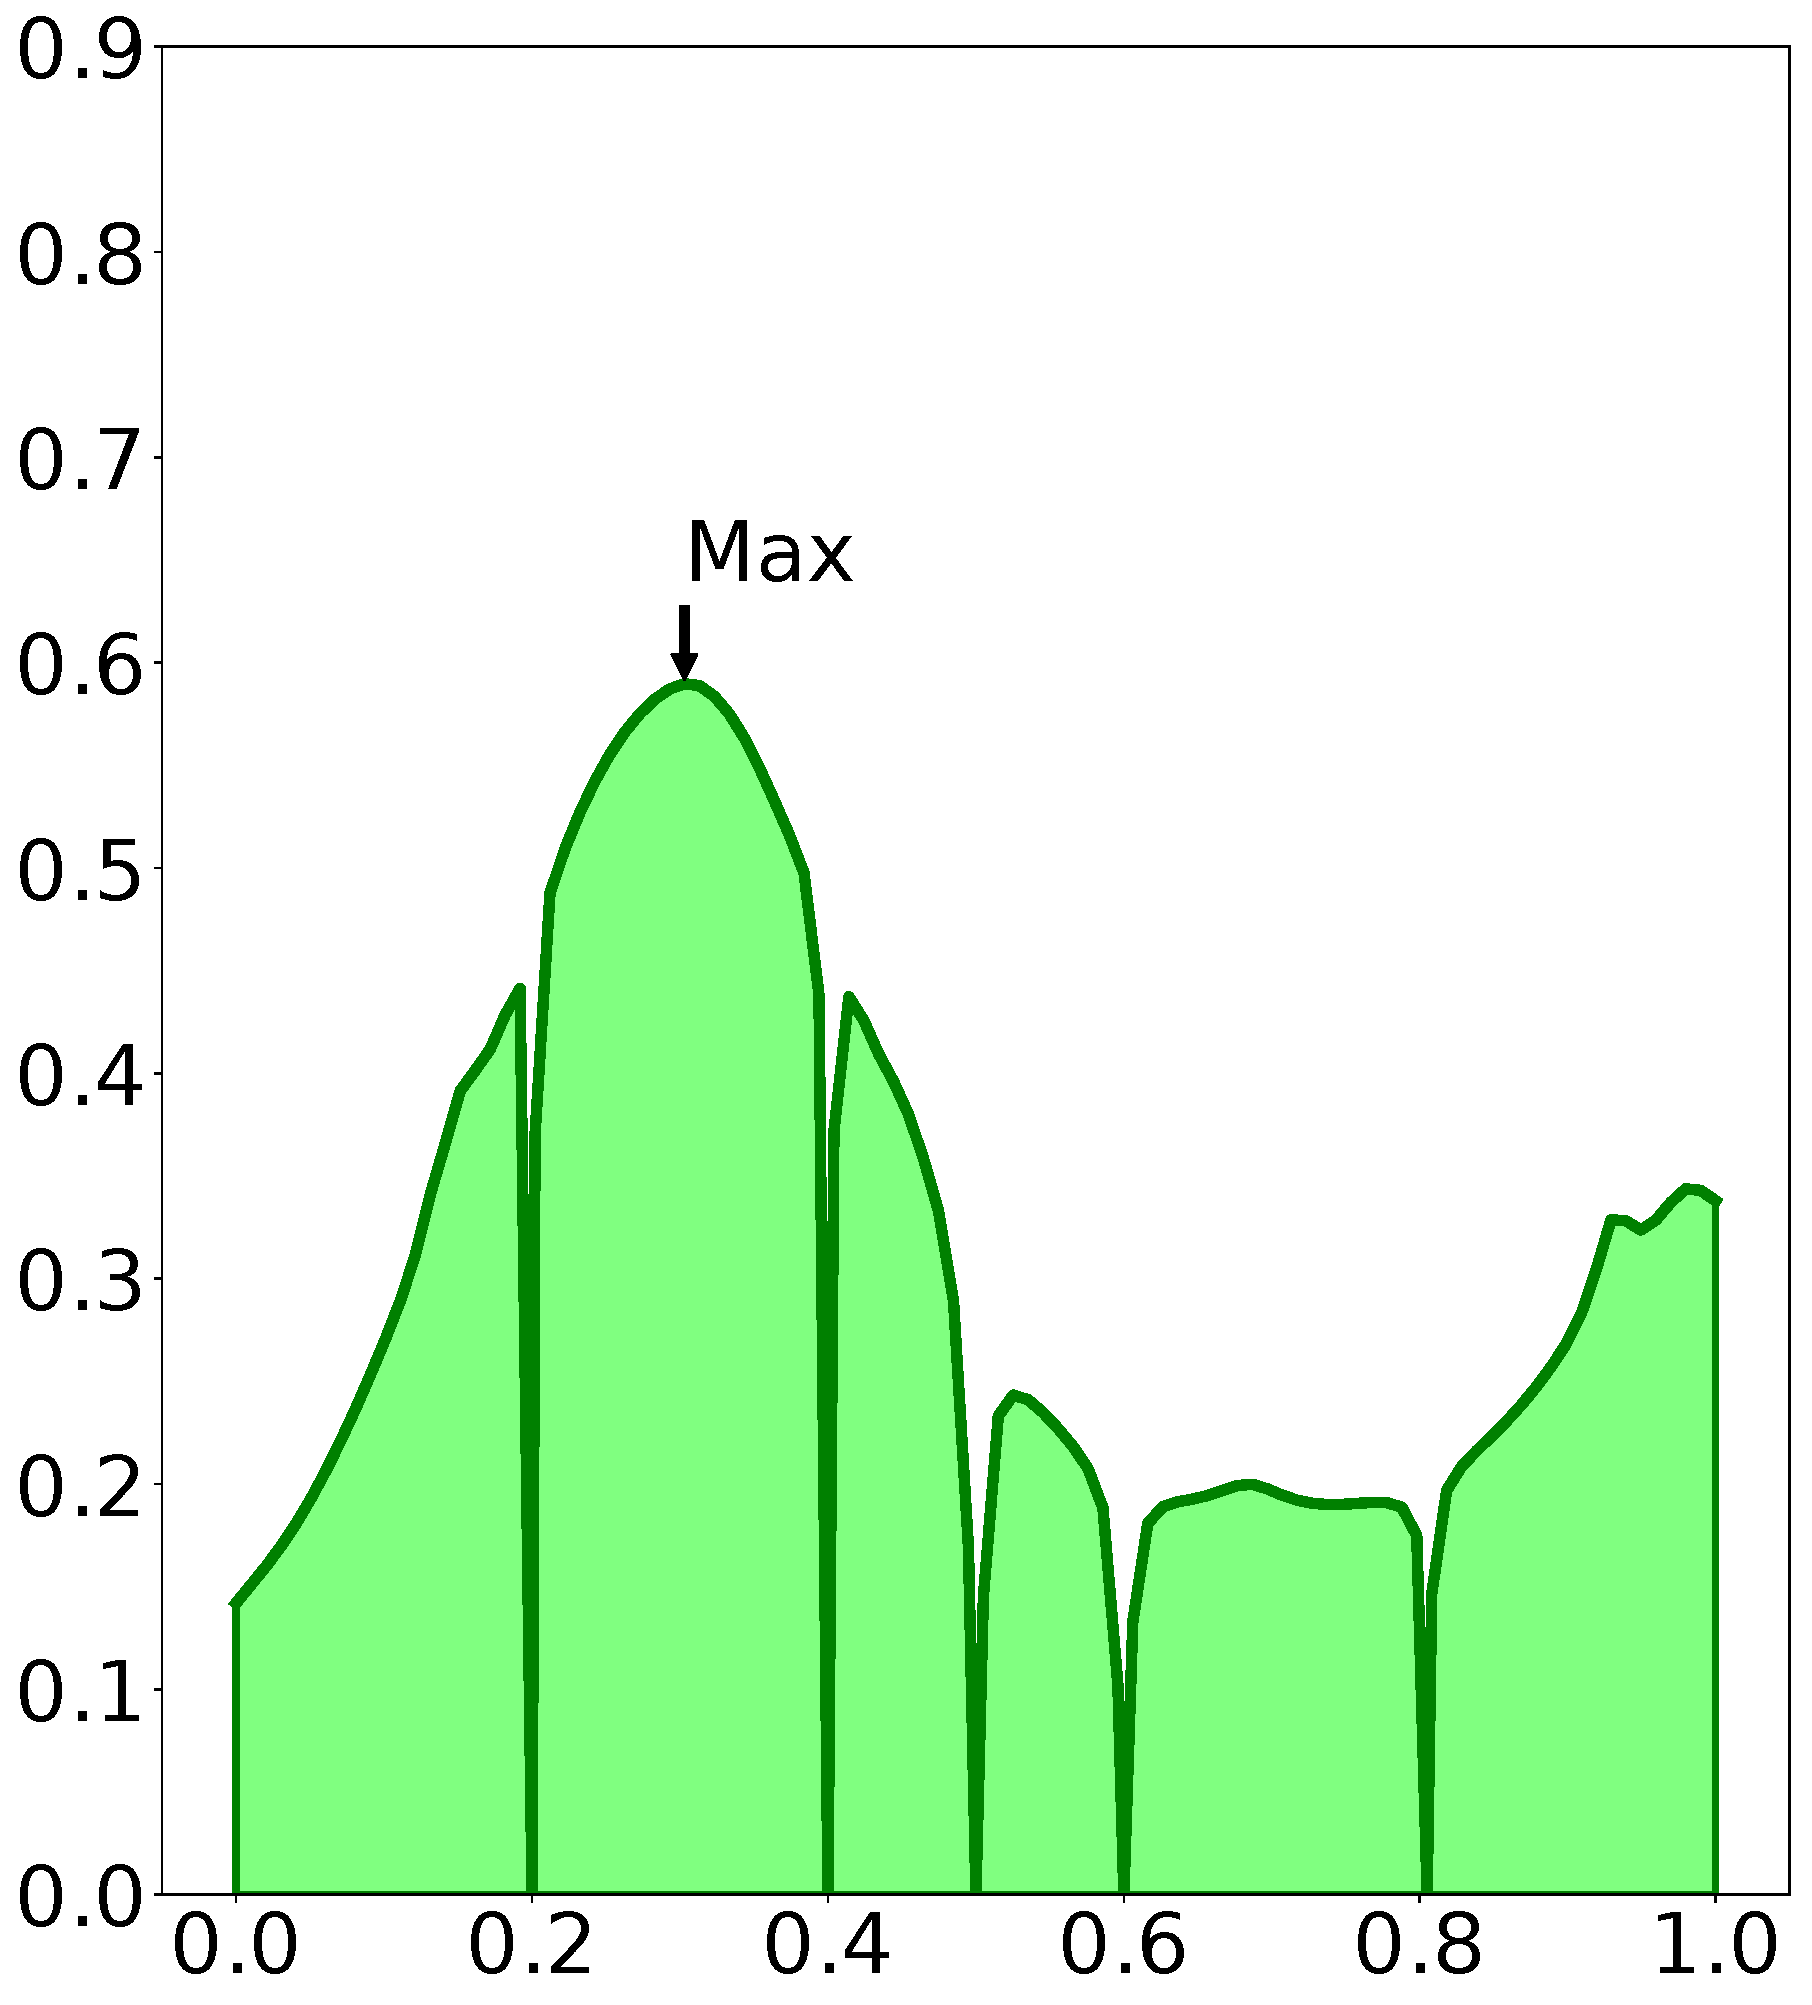
\includegraphics[width=3.4cm,,height=3.9cm]{figures/theory/acq2.pdf} \\
	&
	         {{\footnotesize $\mathbf{s}_1^\text{PD}(\mathbf{x})$}}
        &
                {{\footnotesize Sample of $\mathcal{X}^\star$}}
        &
                {{\footnotesize $\mathbf{s}_1^\text{CPD}(\mathbf{x}|\mathcal{X}^\star_1)$}}
        &
                {{\footnotesize $\alpha_1^\text{const}(\mathbf{x})$}} \\

	\rotatebox{90}{\hspace{1.5cm}$c_1(\mathbf{x})$} &
	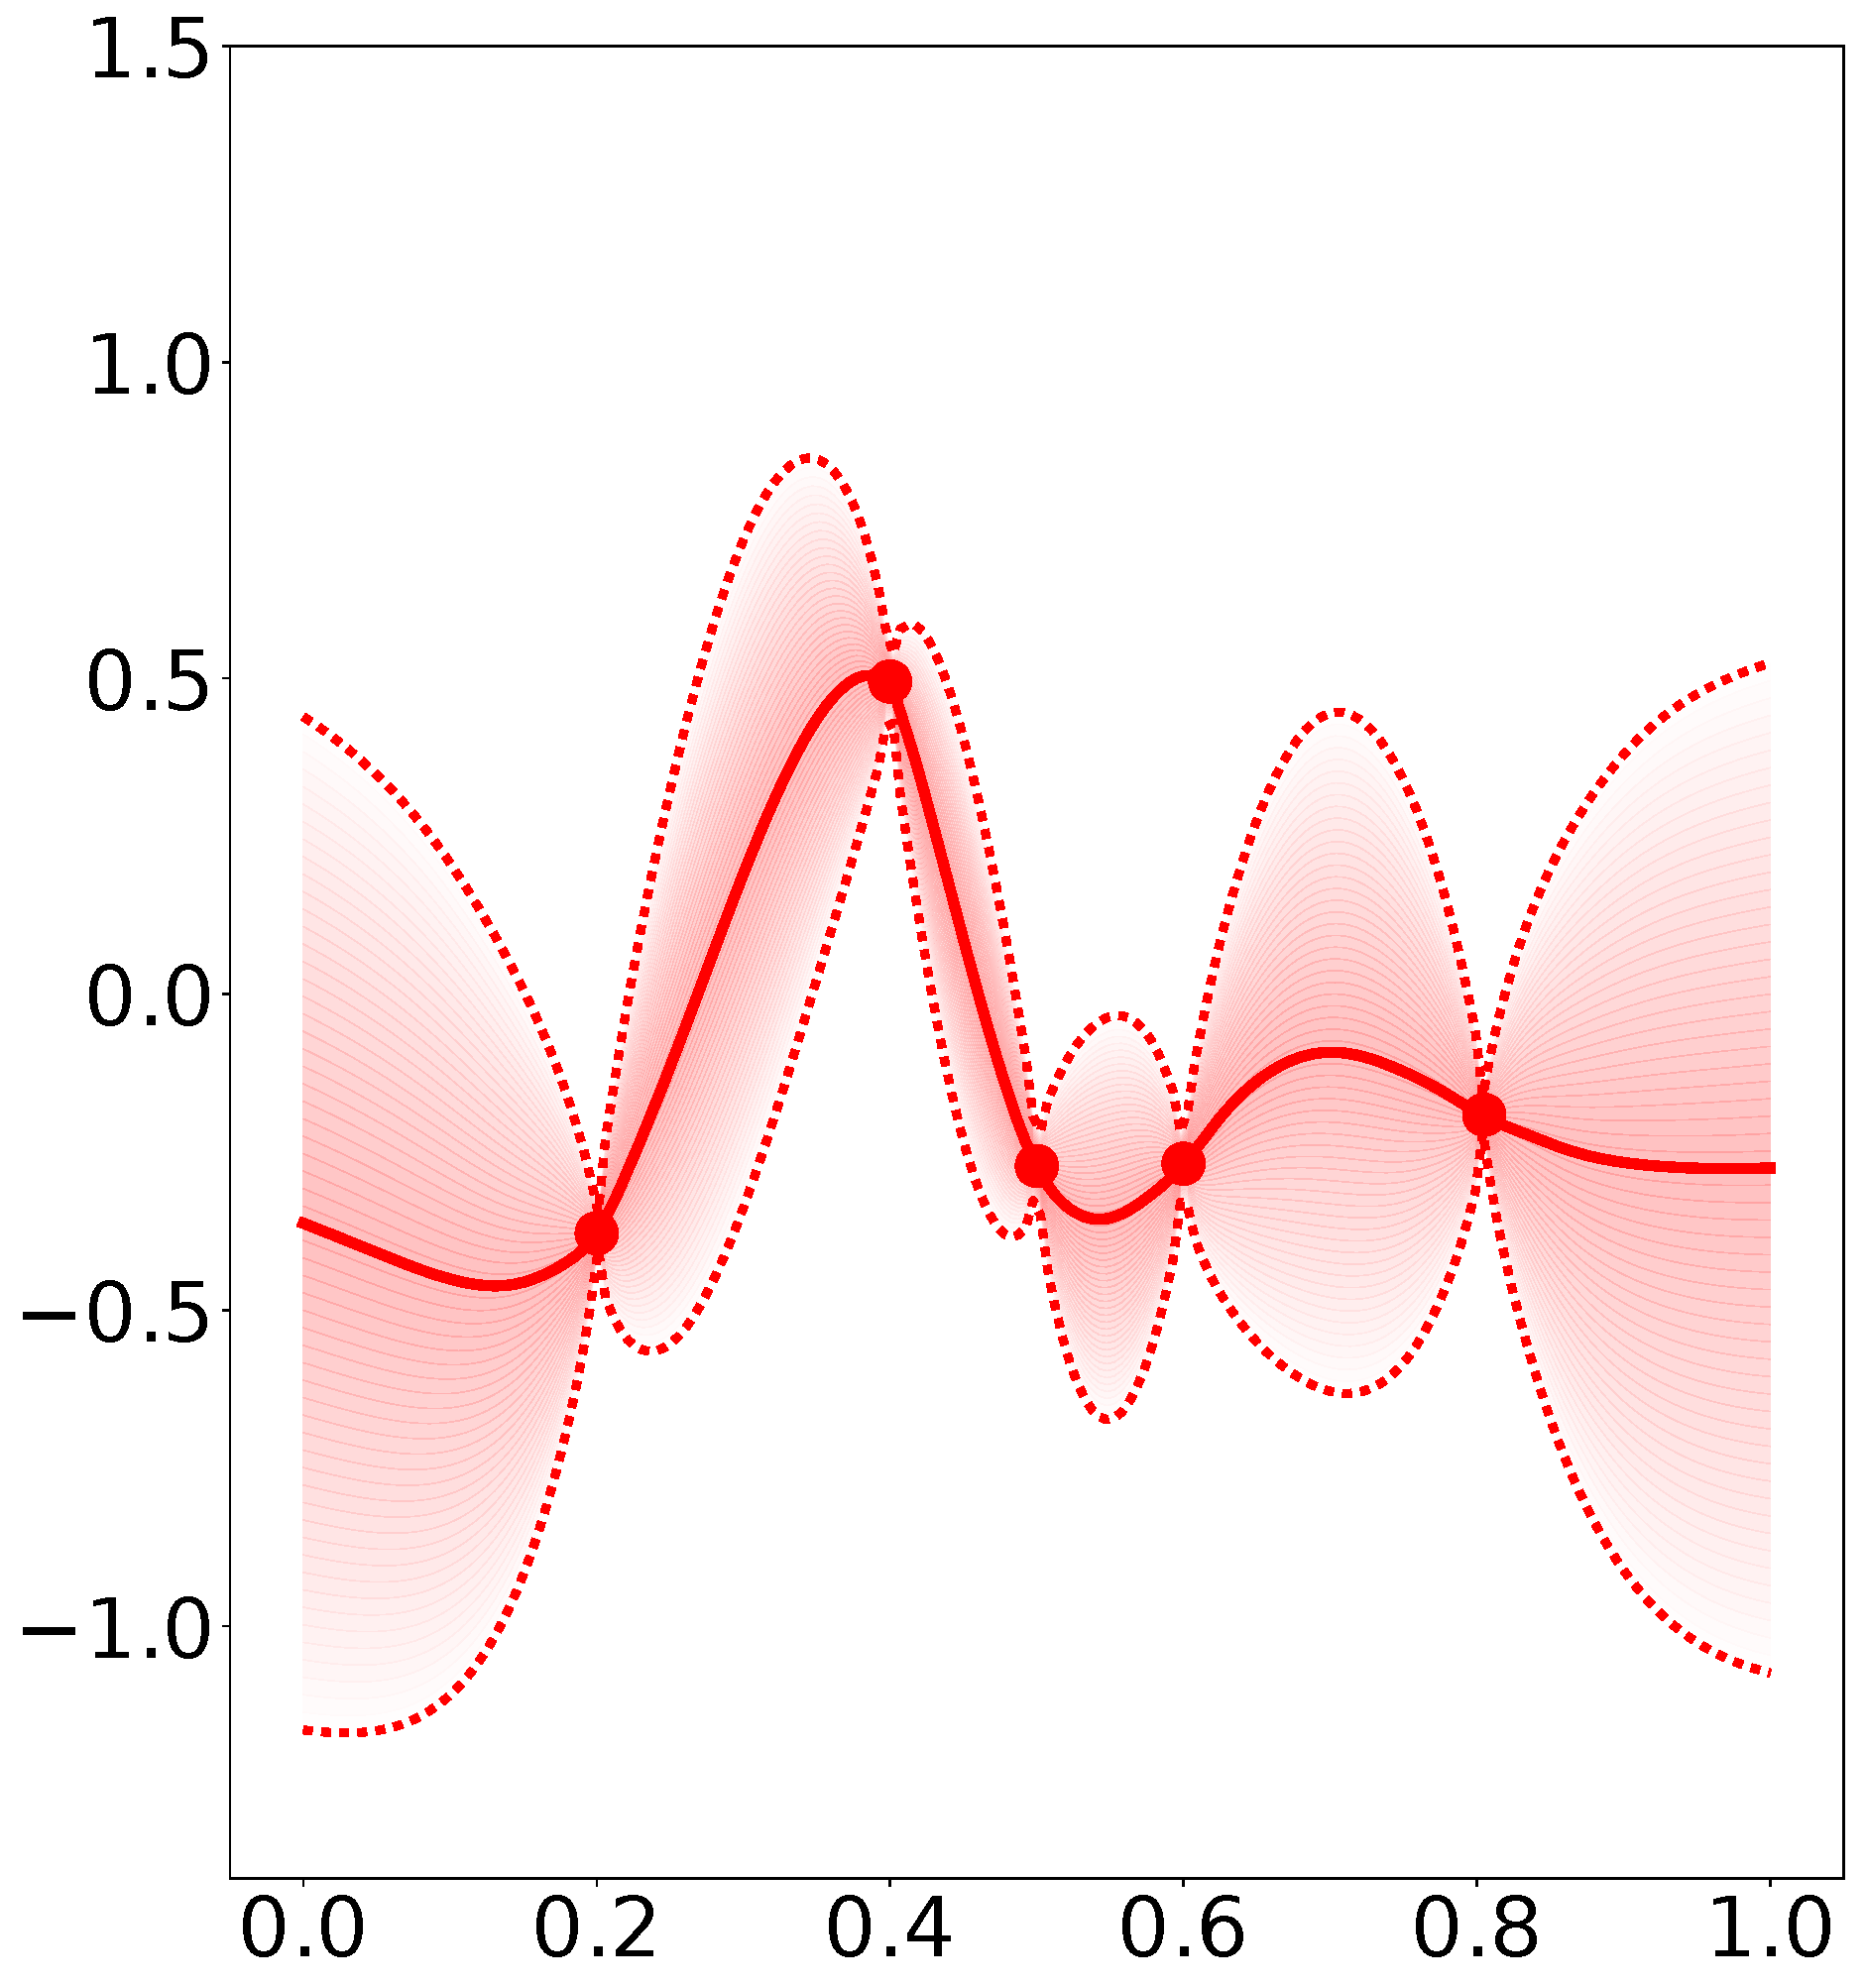
\includegraphics[width=3.4cm,,height=3.9cm]{figures/theory/pred3.pdf}  &
        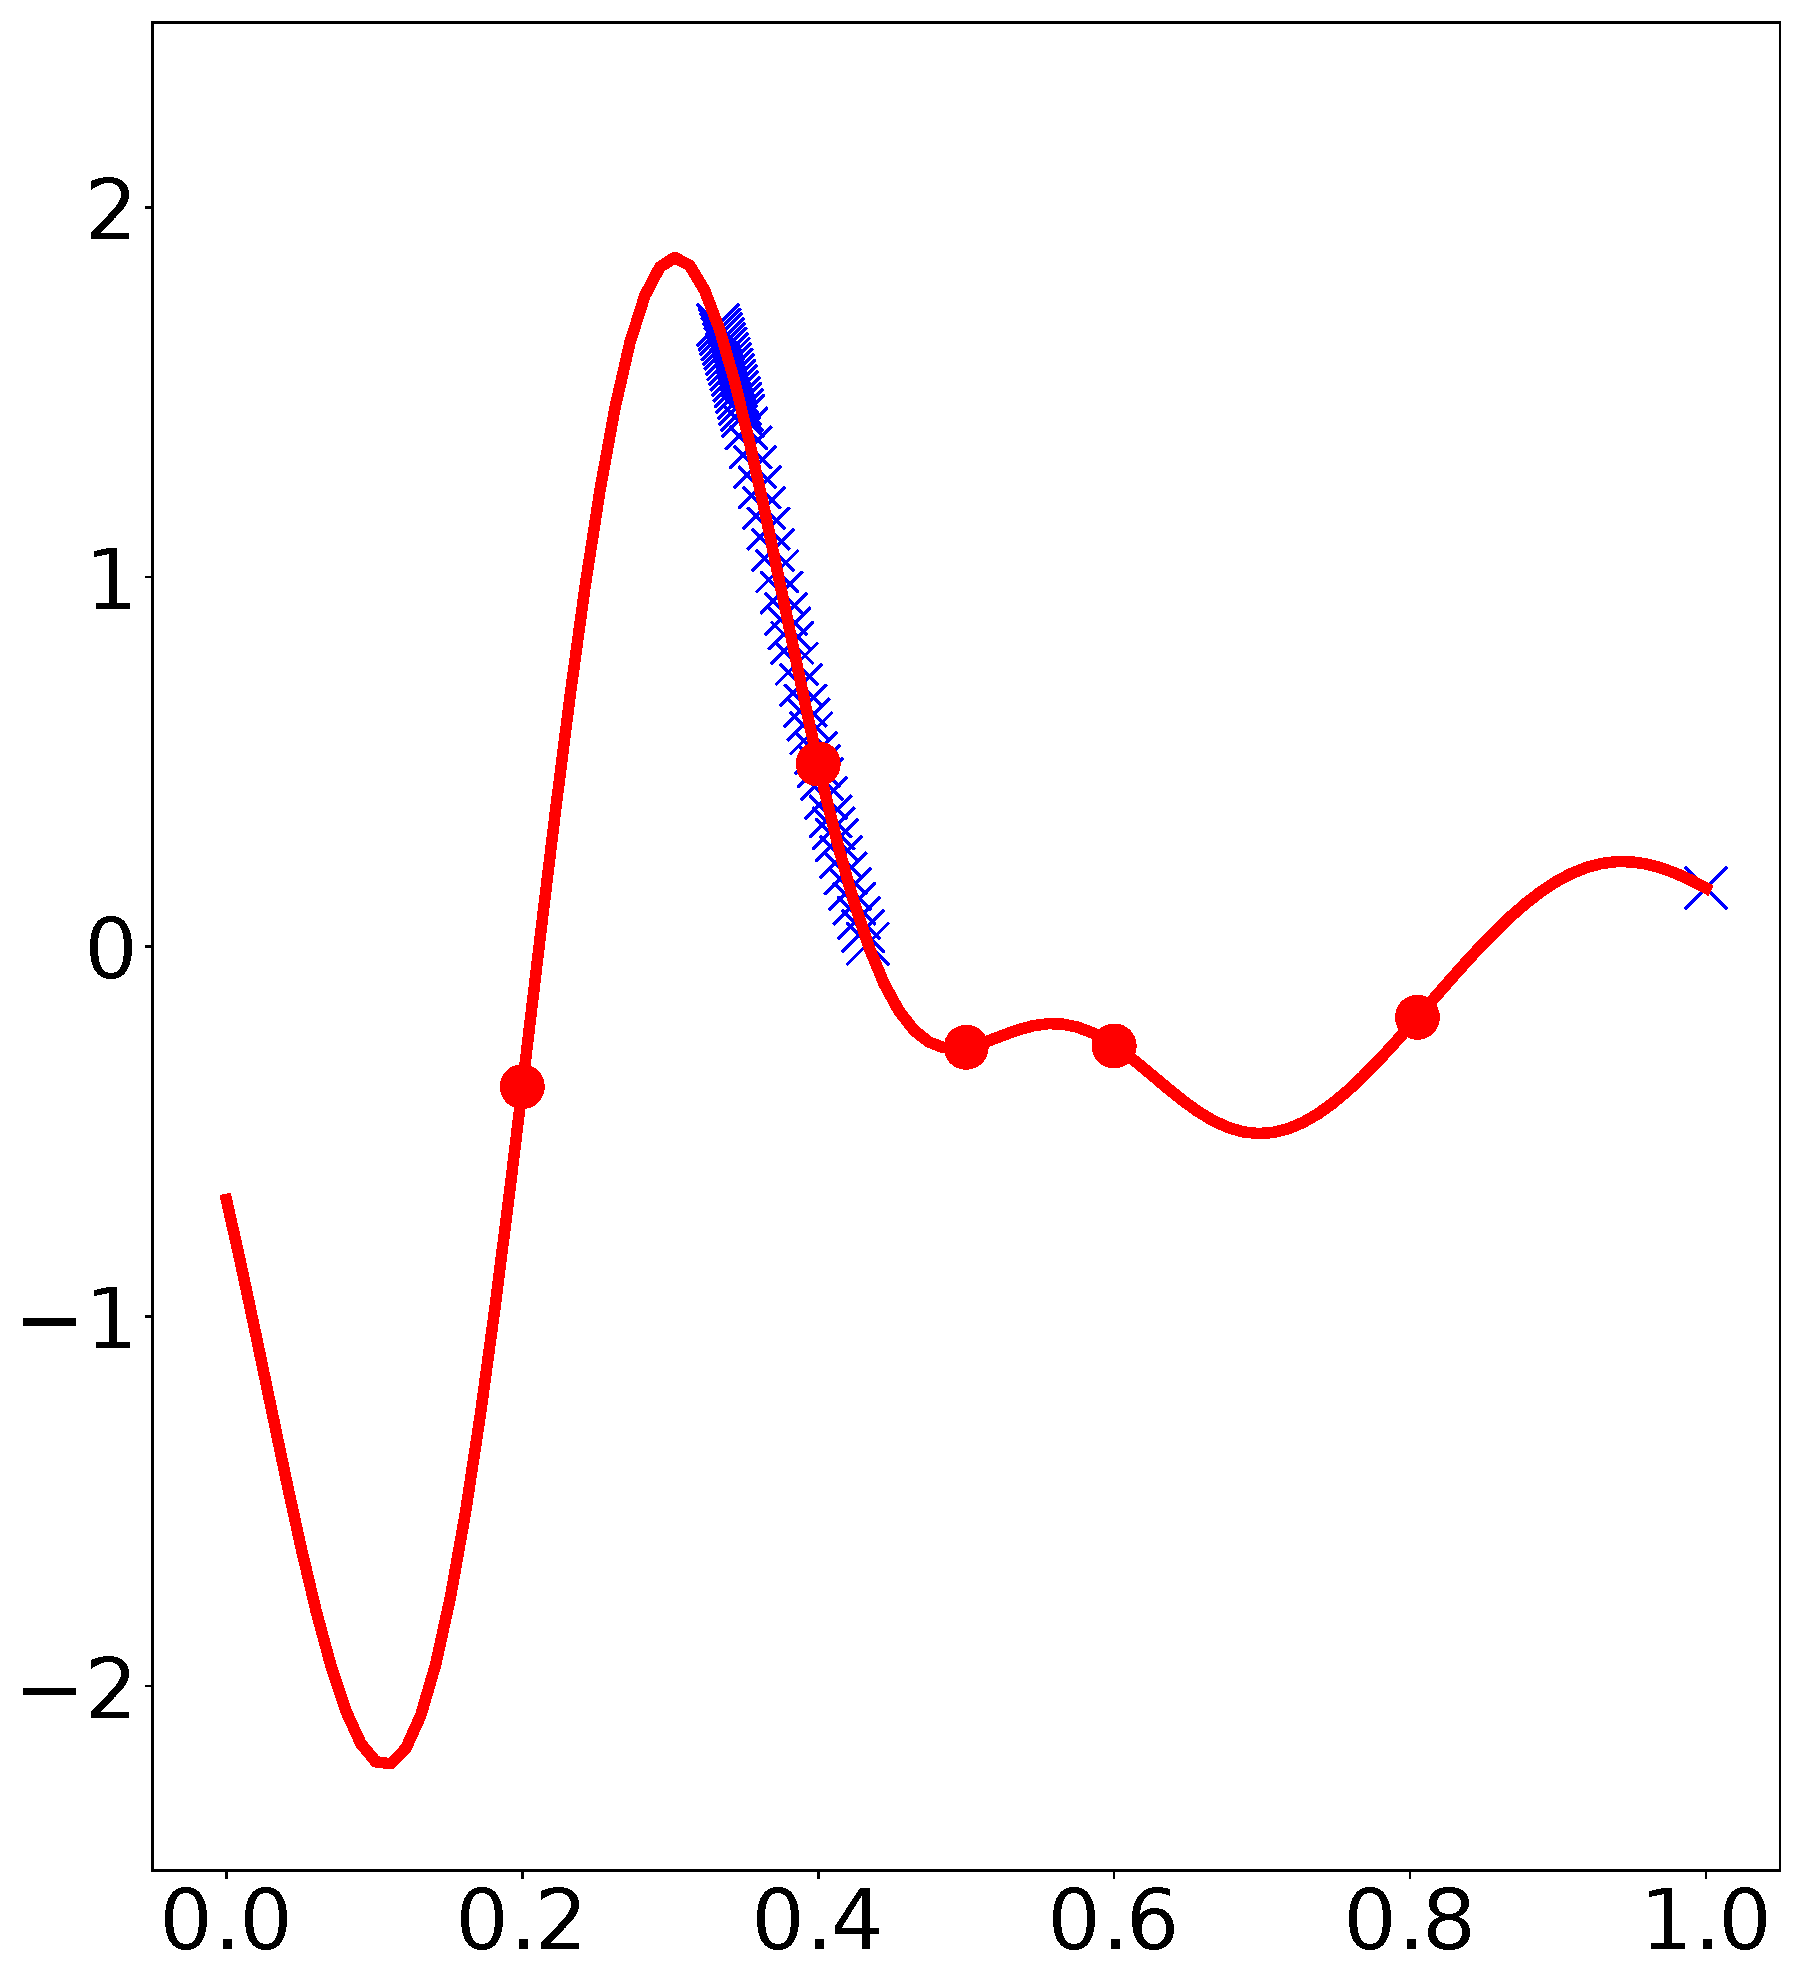
\includegraphics[width=3.4cm,,height=3.9cm]{figures/theory/sample3.pdf} &
	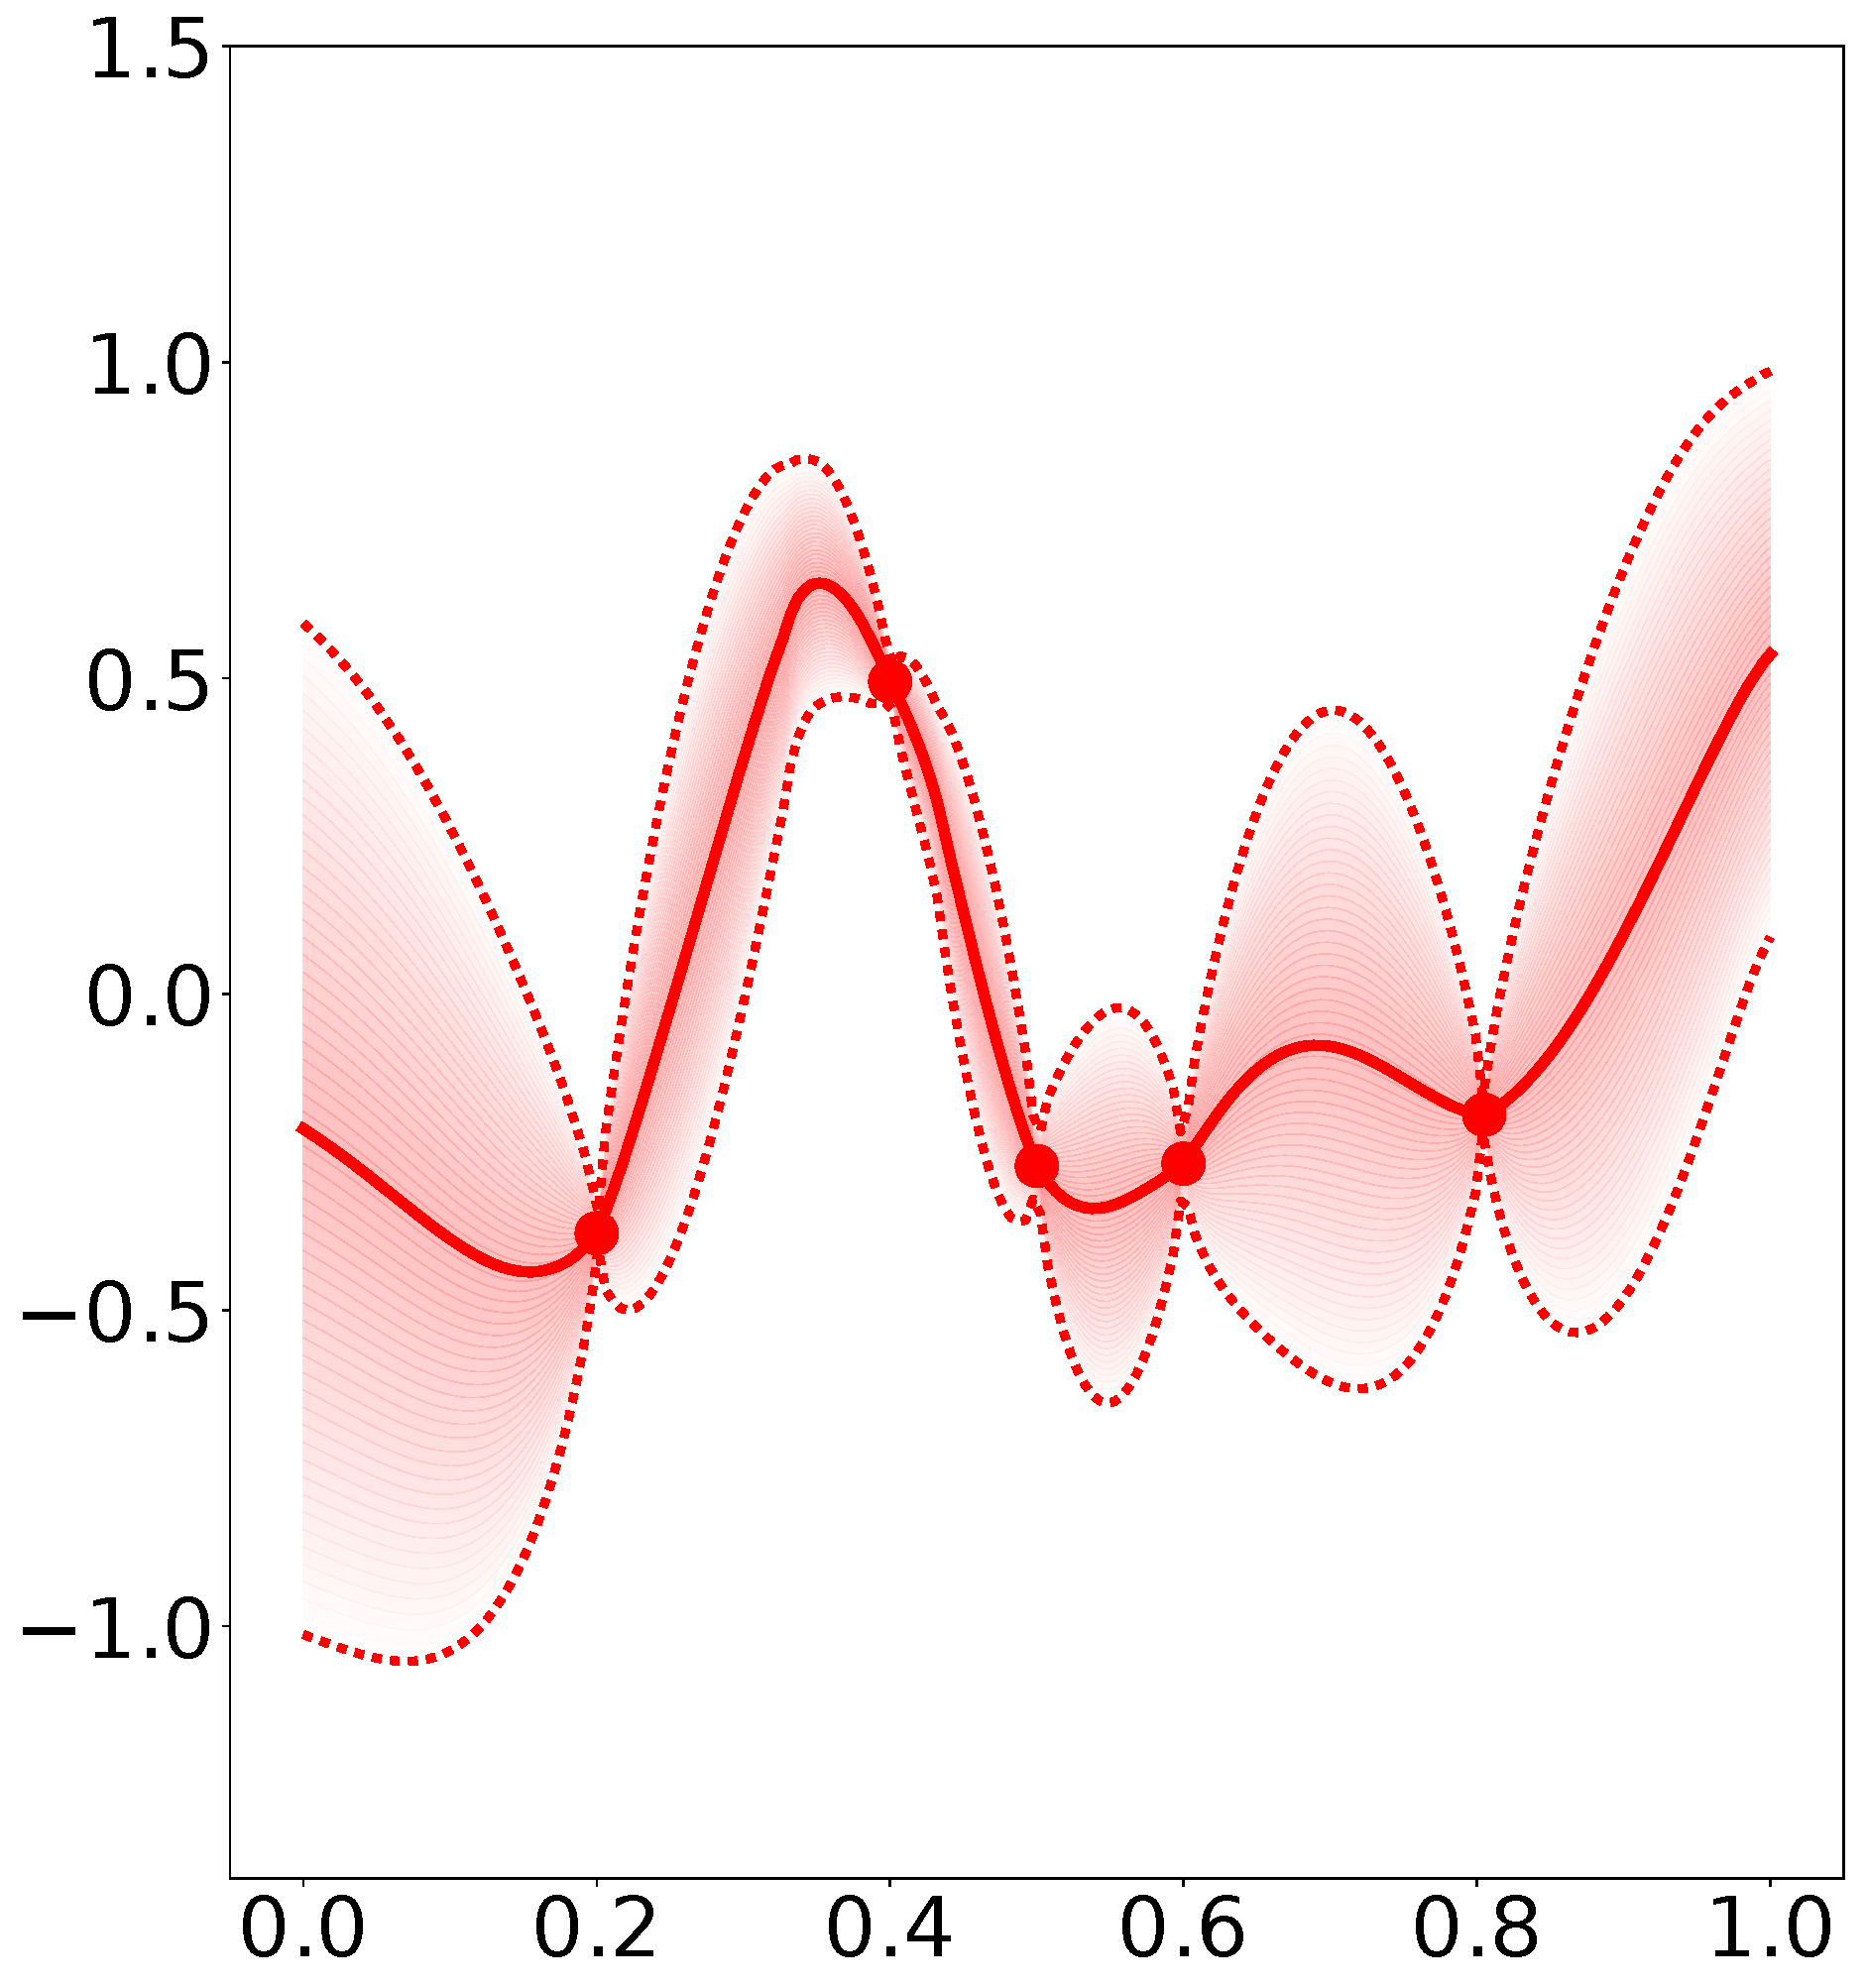
\includegraphics[width=3.4cm,,height=3.9cm]{figures/theory/cond_pred3.pdf} &
        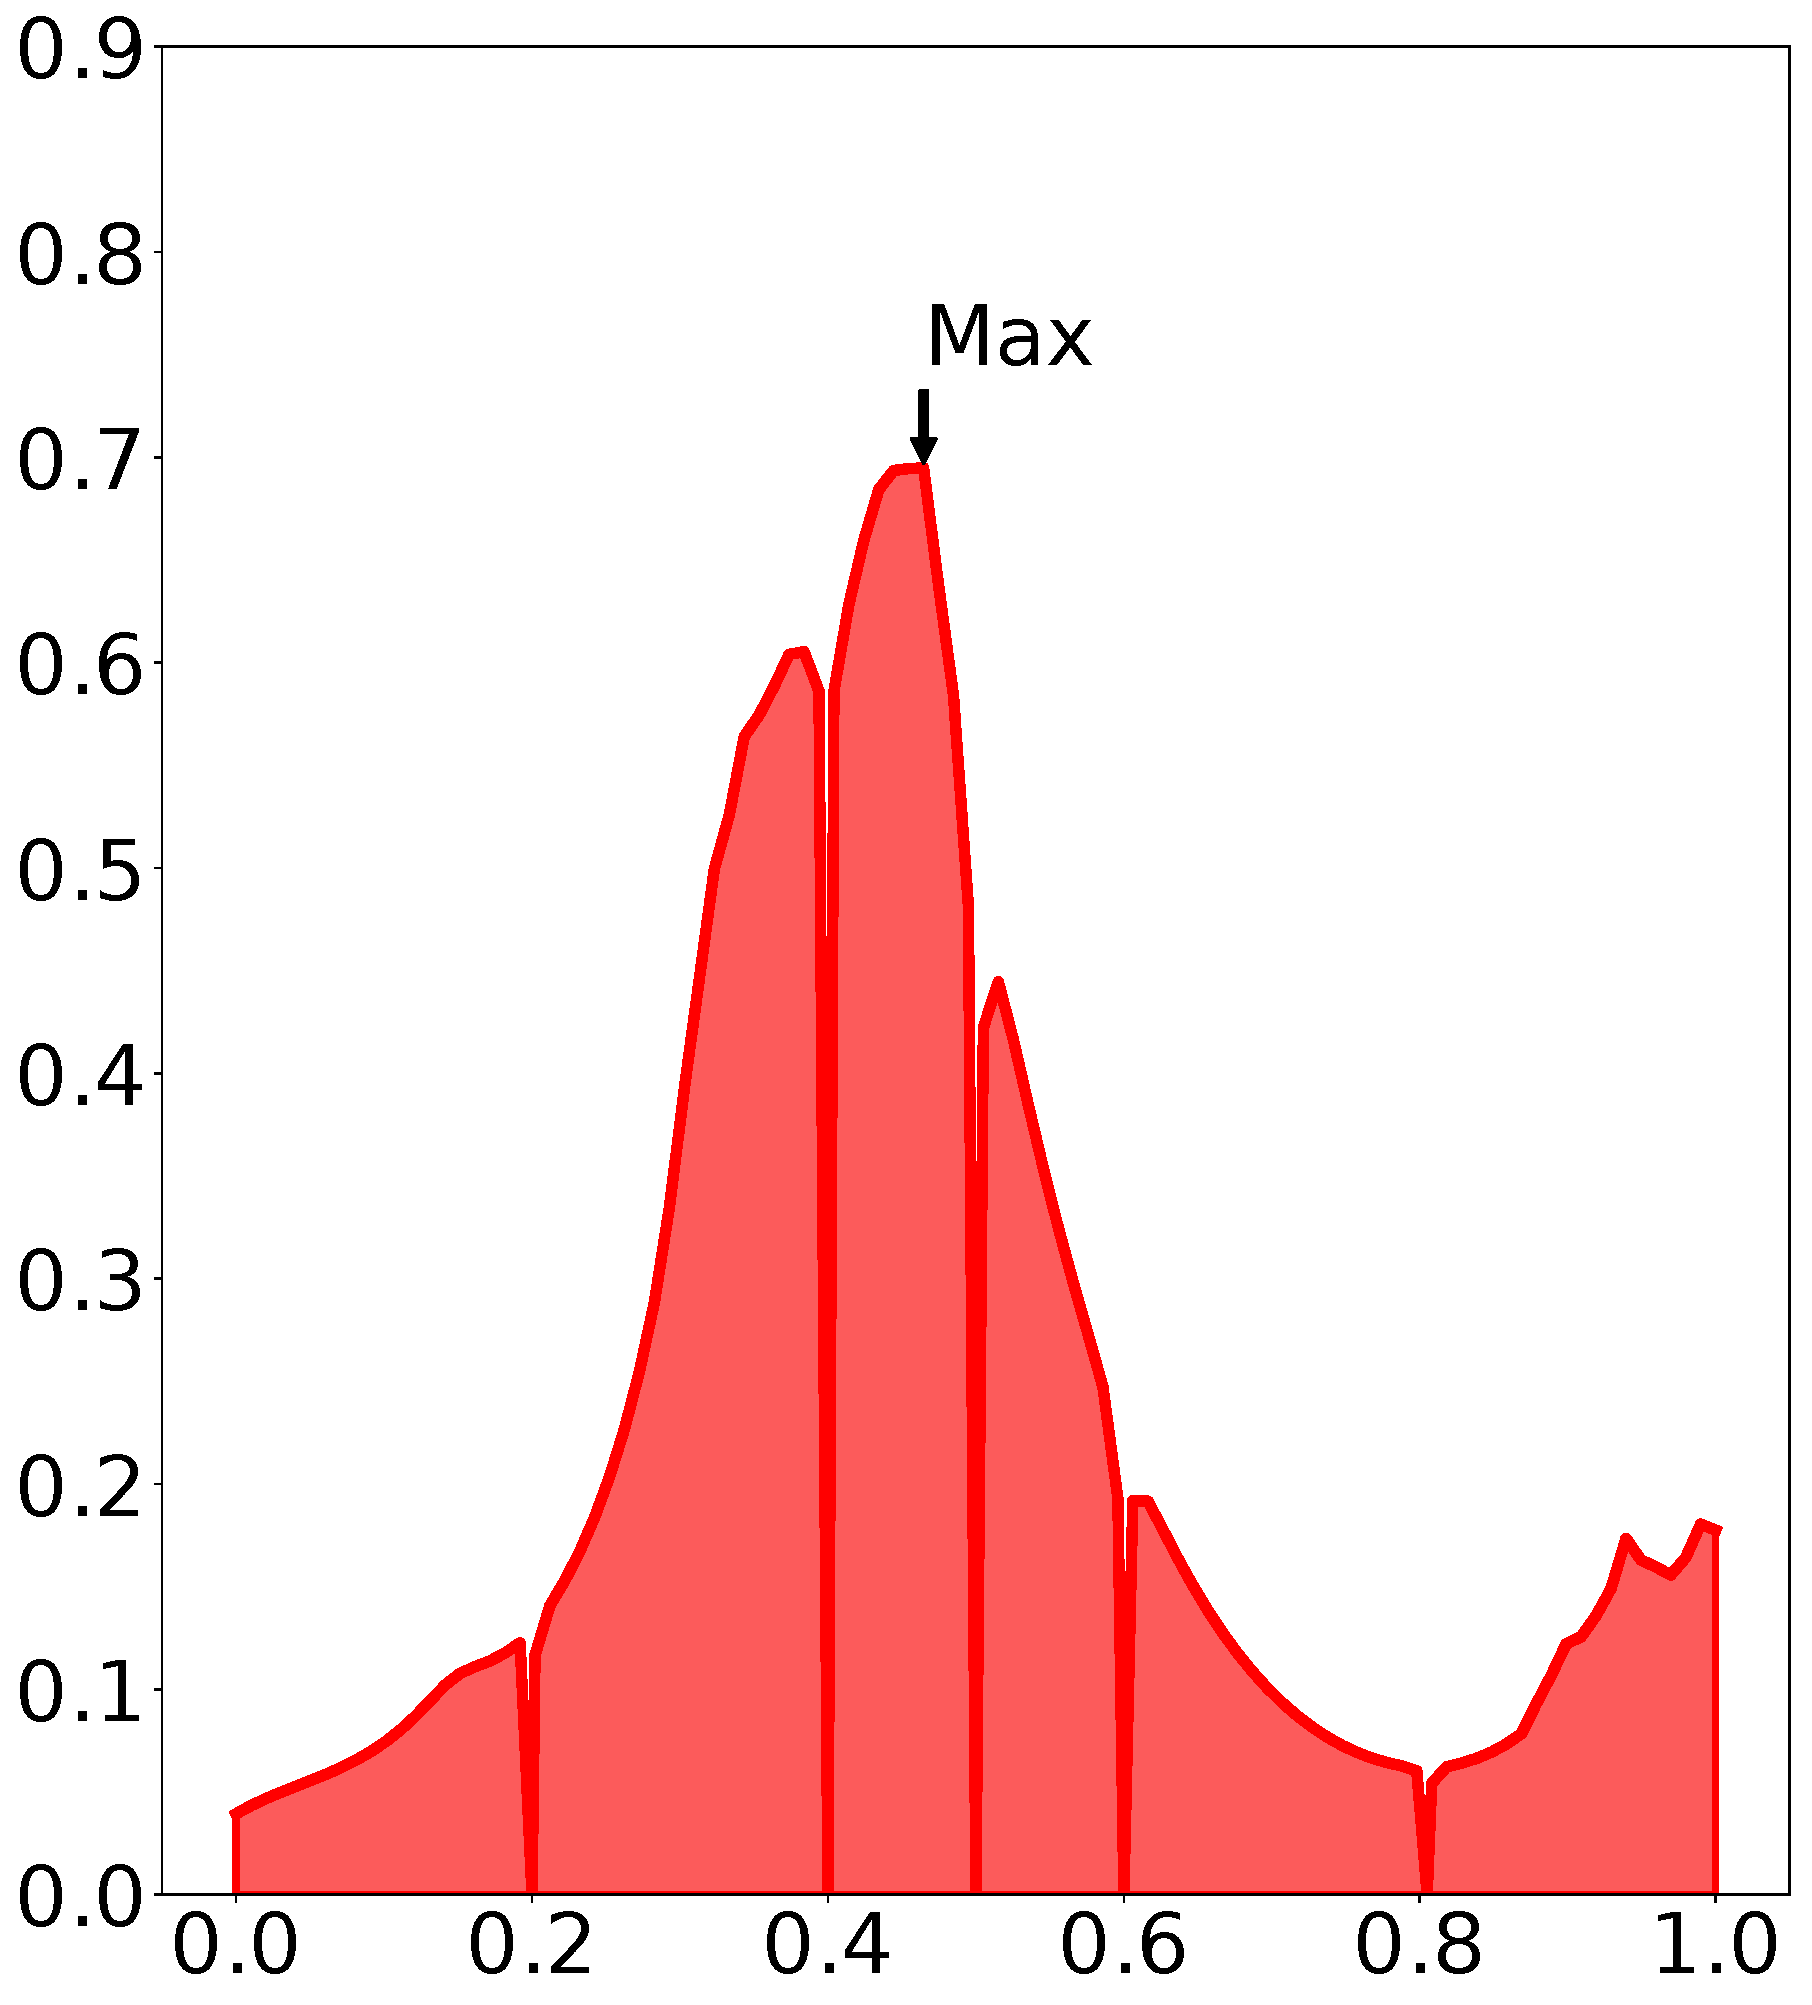
\includegraphics[width=3.4cm,,height=3.9cm]{figures/theory/acq3.pdf} 
\end{tabular}
\caption{Different steps needed to compute PESMOC's acquisition function in a decoupled evaluation scenario. 
	{\bf (first column)} Predictive distribution for each black-box function conditioned on the observed data given by a GP. 
	{\bf (second column)} Sample from the posterior distribution of each GP alongside with the corresponding Pareto set $\mathcal{X}^\star_{(m)}$ 
	in the feasible space displayed using blue crosses. {\bf (third column)} Predictive distribution of each black-box function 
	conditioned to the sampled Pareto set $\mathcal{X}^\star_{(m)}$ being the solution to the optimization problem.
	{\bf (fourth column)} Acquisition function obtained by the difference in the entropy of the predictive distribution before and after
	the conditioning.}
        \label{fig:pesmoc_shape}
\end{center}
\end{figure}

\begin{figure}[t]
\begin{center}
\begin{tabular}{cc}
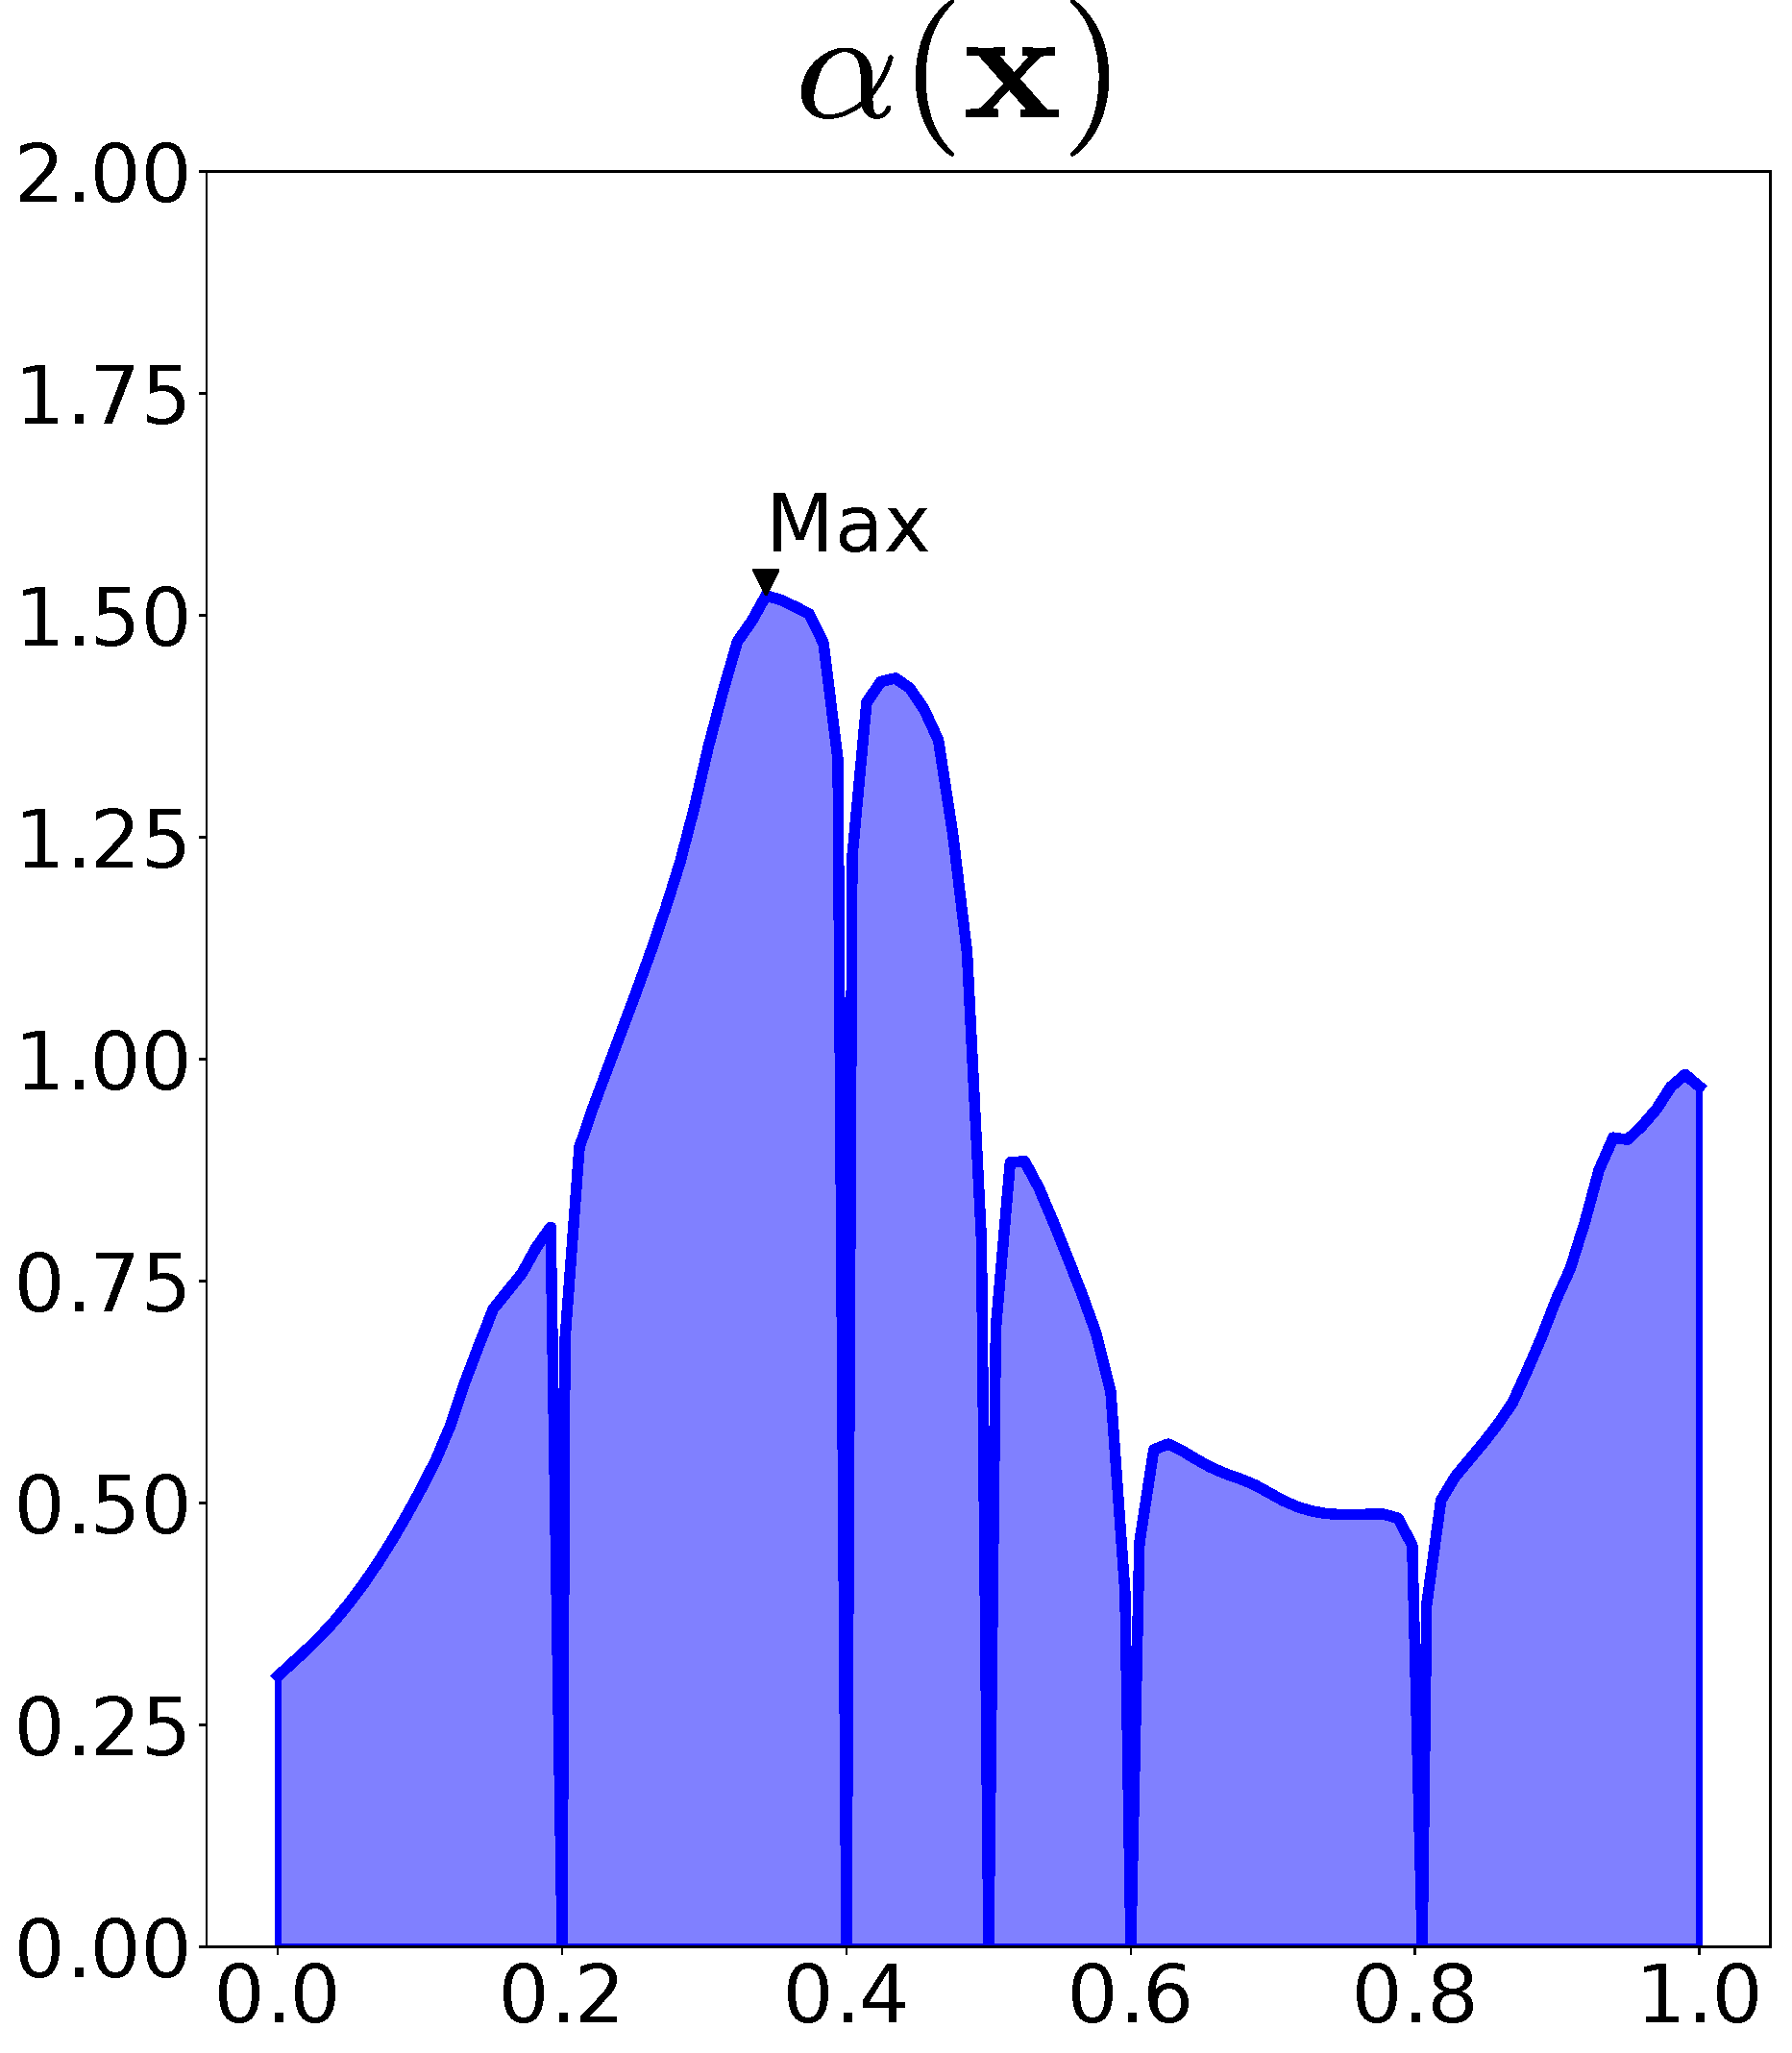
\includegraphics[width=0.3\linewidth]{figures/theory/acq.pdf}
\end{tabular}
\caption{Acquisition function of PESMOC for the coupled setting. In this case $\alpha(\cdot)$ is simply the sum 
	of the acquisition functions of the three black boxes shown in Figure \ref{fig:pesmoc_shape}, in which  the decoupled 
	approach was displayed. }
        \label{fig:pesmoc_coupled_shape}
\end{center}
\end{figure}

\subsection{Computational Cost of PESMOC's Acquisition Function}

The cost of running EP and evaluating the acquisition function is $\mathcal{O}((K+C)q^3)$, 
where $q = N + |\mathcal{X}_{(m)}^{\star}|$, and $N$ is the number of observations collected so far, 
$K$ is the number of objectives and $C$ is the number of constraints. 
In practice EP is run only once per sample of the Pareto set $\mathcal{X}_{(m)}^{\star}$ because  
it is possible to re-use the factors that are independent of the candidate location $\mathbf{x}$ at which the acquisition
function has to be evaluated. Thus, the complexity of computing the predictive variance is 
$\mathcal{O}((K+C)|\mathcal{X}_{(m)}^{\star}|^3)$. In practice, we set the size of the Pareto set 
sample $\mathcal{X}_{(m)}^{\star}$ to be equal to $50$, making $q$ just a few hundreds at most.
We provide more details in the supplementary material about how 
to the conditional predictive distribution $p(\textbf{y}|\mathcal{D}, \textbf{x}, \mathcal{X}^{\star})$
is obtained after running EP.

\section{Related Work}
\label{sec:related}

In this section we review important related work to multi-objective optimization under the presence
of several constraints, when both the objectives and the constraints can be regarded as black-boxes. 
We also describe related methods for Bayesian optimization and previous approaches that also allow for 
decoupled evaluations.

\subsection{Evolutionary Strategies and Meta-heuristics}

The problem of constrained multiobjective optimization where the analytical form of 
the objectives or the constraints is unknown has been already tackled in the literature. 
In order to solve these problems one can employ evolutionary 
strategies such as the ones described in \citep{fonseca1998multiobjective,cai2006multiobjective}. 
Similarly, other techniques adapted to this scenario include particle swarm 
optimization \citep{coello2004handling} or ant colony optimization \citep{alaya2007ant}.
These techniques perform a search in the target space guided 
by some criterion that tries to find the best trade-off between exploration of 
good solutions far away from the regions already explored, and exploitation of the best 
known solutions. The problem of these techniques, also known as meta-heuristics, is that 
they usually require a large number of evaluations in order to achieve good results. 
This is un-affordable in our scenario in which the black-box functions are expected
to be very expensive to evaluate. BO methods, which exploit the information provided
by the probabilistic models to make intelligent decisions about where to evaluate next
these functions, will perform much better in a scenario that includes a limited 
evaluation budget (a few hundred evaluations at most). Empirical 
evidence supporting this is found, for example, in \citep{lobato16_accelerator,mlrMBO2017}.

\subsection{Related Bayesian Optimization Methods}

In the literature most BO methods have traditionally focused on the un-constrained single objective
scenario. A comprehensive summary of different works targeting this type of problems can be found
in \citep{brochu2010tutorial,shahriari2016taking}. 
The first BO methods based on entropy search were proposed to address these simple optimization problems 
\citep{hennig2012entropy,villemonteix2009informational}. The corresponding re-formulation 
based on predictive entropy search in such a setting is described in \citep{hernandez2014predictive}.
This reformulation provides an approximation of the acquisition function of entropy search that 
is more accurate, as the required computations are simplified significantly, and that also leads 
to better optimization results in practice. In any case, all these works can only optimize a single objective under no constraints.

The multi-objective case in which several objectives need to be simultaneously optimized in 
an un-constrained scenario has also received the attention of the BO community. In particular, several BO methods have been 
proposed to address these problems, including ParEGO, SMS-EGO, expected hyper-volume improvement 
(EHI) and sequential uncertainty reduction (SUR) 
\citep{knowles2006parego,ponweiser2008multiobjective,emmerich2008computation,picheny2015multiobjective}.
A multi-objective BO method based on using entropy search and the corresponding re-formulation 
based on predictive entropy search is described in \citep{hernandez2016predictive}. However, such a 
method cannot consider constraints. The work described here is a natural extension that allows to 
incorporate several constraints to the multi-objective problem. Importantly, this extension is not 
trivial since it involves the use of more complicated factors in the computation of the conditional 
predictive distribution. Furthermore, the EP update operations required to compute the approximation 
of the acquisition function are also more arduous.

The problem of optimizing a single objective under several constraints has also been considered
by the BO community. The methods proposed with this goal include variants of the expected improvement (EI)
acquisition function in which one simply chooses the point that is expected to improve the most the best observed 
result so far. For example, the expected improvement with constraints (EIC) \citep{Schonlau98,parr2013,snoek2013,
gardner2014bayesian,gelbart2014bayesian}. A method that is able to tackle this type of problems and that 
is based on entropy search and the corresponding reformulation using predictive entropy search has also 
been proposed in \citep{hernandez2015predictive,hernandez2016general}. Such a method, however, cannot optimize
several objectives at the same time, unlike PESMOC, the method described in this paper. Optimizing several objectives 
at the same time is a significantly more complicated problem. In particular, when the objectives are conflictive, 
the solution to the optimization problem is a set of points, the Pareto set in the feasible space, of potentially 
infinite size.

\subsection{Bayesian Multi-Objective Optimization}

A BO method proposed in the literature to optimize several objectives
under several constraints is Bayesian Multi-objective optimization (BMOO) 
\citep{feliot2015bayesian}. Such a method is based on the expected 
hyper-volume improvement acquisition function (EHI) \citep{emmerich2008computation}, in which 
the expected increase in the hyper-volume is computed after performing an evaluation of 
the black-box functions at a particular input location. The hyper-volume is simply the volume 
of points in functional space above the Pareto front (\emph{i.e.}, the function values associated 
to the Pareto set), which is maximized by the actual Pareto set.
It is hence a natural measure of quality or utility of the current solution of the 
multi-objective problem. When several constraints are introduced in the problem, this criterion boils down to 
the product of a modified EHI criterion (where only feasible points are considered) and the probability of 
feasibility, as indicated by the probabilistic models. Importantly, the utility function
of this acquisition function (the acquisition is simply the expectation of the utility function under 
the predictive distribution of the probabilistic models) is constant (equal to zero) as long as no feasible 
point has been observed. Therefore, it is not an appropriate utility function for heavily constrained problems, where 
finding feasible points is sometimes the main difficulty. As indicated by \cite{feliot2015bayesian}, not all 
unfeasible points are equivalent. A point that does not satisfy a constraint by a small amount has probably 
more value than one that does not satisfy the constraint by a large amount, and should therefore contribute more 
to the utility.

With the goal of overcoming the limitations described before, \cite{feliot2015bayesian}
propose an extended domination rule to handle objectives and constraints in a unified way.
This domination rule considers both objectives $\mathbf{f}(\mathbf{x}) = (f_1(\mathbf{x}),\ldots,f_n(\mathbf{x}))$ and 
constraints $\mathbf{c}(\mathbf{x}) = (c_1(\mathbf{x}),\ldots,c_m(\mathbf{x}))$.
For this, the space of potential objective values $\mathbf{f}(\mathbf{x}) \in \mathcal{Y}_o\subset \mathds{R}^K$ and the space of 
potential constraint values $\mathbf{c}(\mathbf{x}) \in \mathcal{Y}_c \subset \mathds{R}^C$ are joined, giving as a result
the extended space $\mathcal{Y}_o \times \mathcal{Y}_c$. 
Define $\mathbf{y}_\mathbf{x}^o=\mathbf{f}(\mathbf{x})$ and 
$\mathbf{y}_\mathbf{x}^c=\mathbf{c}(\mathbf{x})$. That is $\mathbf{y}^o_\mathbf{x}$ is a vector with the objective values associated to 
$\mathbf{x}$ and $\mathbf{y}^c_\mathbf{x}$ is a vector with the constraint values.
The extended domination rule states that a point $\mathbf{x}$ dominates another one $\mathbf{x}'$,
if $\Psi(\mathbf{y}_\mathbf{x}^o,\mathbf{y}_\mathbf{x}^c)$ dominates $\Psi(\mathbf{y}^o_{\mathbf{x}'}, 
\mathbf{y}^c_{\mathbf{x}'})$, using the classical 
Pareto domination rule. That is, $\Psi(\mathbf{y}_\mathbf{x}^o, \mathbf{y}_\mathbf{x}^c) 
\prec \Psi(\mathbf{y}^o_{\mathbf{x}'}, \mathbf{y}^c_{\mathbf{x}'})$ 
i.f.f $\Psi(\mathbf{y}_\mathbf{x}^o,\mathbf{y}_\mathbf{x}^c)$ is better than $\Psi(\mathbf{y}^o_{\mathbf{x}'}, 
\mathbf{y}^c_{\mathbf{x}'})$ in at least one component. 
Let $\overline{\mathds{R}}$ be the extended real line.
The transformation $\Psi(\cdot, \cdot): \mathcal{Y}_o \times \mathcal{Y}_c \rightarrow \overline{\mathds{R}}^K\times \mathds{R}^C$
is defined as:
\begin{align}
\Psi(\mathbf{y}^o_\mathbf{x},\mathbf{y}^c_\mathbf{x}) = \left\{ \begin{array}{ll}
(\mathbf{y}^o_\mathbf{x},\mathbf{0}) & \mbox{if $\mathbf{y}^c_\mathbf{x} \geq 0$},\\
(+\infty, \min{(\mathbf{y}^c_\mathbf{x},\mathbf{0})}) & \mbox{otherwise.}
\end{array}
\right.
\end{align}
That is, if the point is feasible (\emph{i.e.}, all the constraints are positive or equal to zero), only the objective
values are considered. Conversely, if the point is infeasible, the constraint values will play a role.
More precisely, under this rule a solution that is infeasible but close to being feasible will dominate 
other infeasible solutions that are further away from being feasible.
As described by \cite{feliot2015bayesian}, the previous rule has these properties:
\begin{enumerate}
\item For unconstrained problems the extended domination rule boils down to the classical Pareto domination rule.
\item Feasible solutions (corresponding to $\mathbf{y}^c_\mathbf{x} \geq \mathbf{0}$) are compared using the 
	Pareto domination rule applied in the objective space.
\item Non-feasible solutions (corresponding to $\mathbf{y}^c_\mathbf{x} \ngeq \mathbf{0}$)
	 are compared using the Pareto domination rule applied to the vector of constraint violations.
\item Feasible solutions always dominate non-feasible solutions.
\end{enumerate}

The extended domination rule presented above makes it possible to define a notion of expected hyper-volume
improvement in the extended space. This is the acquisition function considered by \cite{feliot2015bayesian}.
A problem is, however, that evaluating this quantity can be expensive if the number of objectives and constraints 
is large. To overcome this limitation an efficient approximate computation method is proposed by those authors.
This approximation is obtained by noticing that the proposed acquisition function at a candidate point $\mathbf{x}$ 
is given by the expected value of the probability that $\Psi(\mathbf{y}_\mathbf{x}^o,\mathbf{y}_\mathbf{x}^c)$
dominates a point $\mathbf{y}$ belonging to the set of non-dominated points in the extended output space, 
when $\mathbf{y}$ is chosen uniformly at random from that set. In particular,
\begin{align}
\alpha_\text{BMOO}(\mathbf{x}) &= \mathds{E}_{\mathbf{y}_\mathbf{x}^o,\mathbf{y}_\mathbf{x}^c}\left[ \int_{\mathcal{G}_N} 
	I(\Psi(\mathbf{y}_\mathbf{x}^o,\mathbf{y}_\mathbf{x}^c) \prec \mathbf{y}) d \mathbf{y} \right]
	\nonumber \\
	& =  \int_{\mathcal{G}_N} p(\Psi(\mathbf{y}_\mathbf{x}^o,\mathbf{y}_\mathbf{x}^c) \prec \mathbf{y}) d \mathbf{y}
	\nonumber \\
	& \approx \frac{1}{M} \sum_{m=1}^M  p(\Psi(\mathbf{y}_\mathbf{x}^o,\mathbf{y}_\mathbf{x}^c) \prec \mathbf{y}_m)
	\,,
	\label{eq:acc_bmoo}
\end{align}
where $\mathcal{G}_N$ is the set of non-dominated points (up to the current iteration $N$) in the 
extended output space; $I(\cdot)$ is an indicator function;
the expectation is given by the predictive distribution of the probabilistic models fitting each objective and constraint;
$p(\Psi(\mathbf{y}_\mathbf{x}^o,\mathbf{y}_\mathbf{x}^c) \prec \mathbf{y})$ is the probability that
$\Psi(\mathbf{y}_\mathbf{x}^o,\mathbf{y}_\mathbf{x}^c)$ dominates $\mathbf{y}$ and $M$ is the number of samples for 
$\mathbf{y} \in \mathcal{G}_n$ used in the approximation. Importantly, there is a closed form expression for 
$p(\Psi(\mathbf{y}_\mathbf{x}^o,\mathbf{y}_\mathbf{x}^c) \prec \mathbf{y})$ when the probabilistic 
models are Gaussian processes. The only problem is hence how to generate uniform variables over the set $\mathcal{G}_N$.

To generate the samples required in (\ref{eq:acc_bmoo}) \cite{feliot2015bayesian} propose a Monte Carlo method based
on the Metropolis-Hastings algorithm targeting the uniform distribution in $\mathcal{G}_{N}$. At each iteration of this 
algorithm the current samples (particles) are slightly perturbed. This step is only accepted if the new
particle falls in $\mathcal{G}_{N}$ . Of course, when a new observation is obtained, improving the current solution, 
the set $\mathcal{G}_{N+1}$ has a smaller size than $\mathcal{G}_{N}$. Therefore, some particles may have to be removed. 
\cite{feliot2015bayesian} describe an intelligent method to avoid the elimination of a large number of particles at each 
iteration, which will reduce the quality of the generated samples and the approximation.

In our experiments we have compared the proposed approach, PESMOC, with the BMOO method just described.
We have observed that BMOO suffers from the limitations of traditional methods based on the 
expected improvement (EI). In particular, it often is too greedy and tends to explore the limits of the 
input space too much. In high dimensions this can be a problem since there are a lot of these corners.  
An extra difficulty of BMOO is that, in practice, one has to bound the space of potential output values for the
objectives and the constraints, and this information may not be available before hand.

\subsection{Existing Methods for Decoupled Evaluations}

Decoupled evaluations in a BO setting were first considered by \cite{gelbart2014bayesian} 
for a single objective and several constraints. In that work it is shown that 
the standard acquisition function known as expected improvement
(EI) leads to a pathology that prevents decoupled evaluations. The reason for that is that 
no-improvement over the current best solution (this is the utility function of EI) can occur if we observe 
only the objective or the constraints, separately. More precisely, two conditions are required to produce 
positive values of the utility: (i) the evaluation for the objective must 
achieve a lower value than the best observed feasible solution so far and, (ii), the evaluations 
for the constraints must produce non-negative values. These two conditions 
cannot be simultaneously satisfied by a single observation (objective or constraint). 
Therefore, standard EI cannot be used for decoupled evaluations. The problem described is 
solved by using a two stage process in which standard EI is used to pick-up a candidate point 
$\mathbf{x}_{N+1}$, and then, entropy search is used to choose the black-box function to
evaluate next \citep{villemonteix2009informational}. This approach is 
sub-optimal and a joint selection of $\mathbf{x}_{N+1}$ and the black-box is expected to perform better.

The limitations of the previous method are circumvented in \citep{hernandez2016general}. In particular,
PESC, the strategy described in that paper for single-objective constrained Bayesian optimization, allows
to perform decoupled evaluations that can simultaneously choose $\mathbf{x}_{N+1}$ and the black-box function
to evaluate next. This strategy is also based on predictive entropy search and expectation propagation.
A comprehensive analysis of the decoupled evaluation setting in this type of optimization problems is carried
out in that work. Importantly, two different decoupled configurations are evaluated: (i) competitive decoupling, 
in which the black-boxes compete for a single resource available; and (ii) non-competitive decoupling, in which the 
black-boxes can be evaluated in parallel at different input locations. Only competitive decoupling is 
found to perform significantly better than a coupled evaluation setting.

A decoupled evaluation method for un-constrained multi-objective Bayesian optimization is described in
\citep{hernandez2016predictive}. PESMO, the technique described by those authors, also uses predictive entropy 
search and expectation propagation to choose which black-box function and which input location 
$\mathbf{x}_{N+1}$ to evaluate next. These authors only consider competitive decoupled evaluations. The results obtained 
show that such a setting can significantly outperform coupled evaluations in the multi-objective case. 

The method we propose here, PESMOC, can be seen a natural extension of the two works described above, 
PESC, and PESMO. PESMOC also allows for decoupled evaluations and combines the possibility of considering several 
objectives and several constraints at the same time. Our results also indicate that a decoupled evaluation setting
may have important benefits in the constrained multi-objective case. The method we compare with, BMOO, is based
on a generalization of EI for constrained multi-objective problems. Therefore, this method suffers from the same 
limitations as standard EI for the single-objective constrained setting and cannot be used to perform decoupled evaluations.

PESMOC is significantly different from PESC. In particular, PESC can only provide solutions to
single-objective constrained optimization probems. PESMOC, on the other hand, can be used to find the solution 
of multi-objetive optimization problems under several constraints. When the objectives are conflictive, the solution 
is a set of points, the Pareto set in the feasible space, of potentially infinite size. This makes multi-objective problems significantly more challenging. 

PESMOC also differs from PESMO. In PESMO there are no constraints in the optimizaton problem. Incorporating
constraints in the multi-objective problem is challenging and requires to add extra factors to compute the
conditional predictive distribution described in (\ref{eq:exact_acq}). These extra factors have to be approximated
by expectation propagation (EP), which results in different EP updates from those of PESMO. Furthermore, when computing the 
acquisition funciton one has to take into account the predictive variances of the latent functions corresponding to the constraints.
In PESMO there are no constraints, so they can be ignored. Importantly, when sampling $\mathcal{X}^\star$ in PESMOC one
also needs to consdier the feasible space $\mathcal{F}$ by sampling also the constraints, which must be taken into account when
solving the corresponding optimization problem. This makes the process of sampling $\mathcal{X}^\star$ more complicated in PESMOC. PESMO does not have to 
consider the possibility of having constraints. Finally, when doing a recommendation, PESMOC has to take into account that the 
provided solution must be feasible with high probability, as indicated in Section \ref{sec:experiments}. PESMO does not have to worry 
about this. Summing up, PESMOC can be used to solve a collection of problems that PESMO cannot address.

\section{Experiments}
\label{sec:experiments}

We carry out several experiments to evaluate the performance of PESMOC, the proposed method for 
constrained multi-objective Bayesian optimization. In these experiments we compare coupled evaluations 
and competitive decoupled evaluations. In the second case, we not only choose which is the next input 
location but also which black-box function should be evaluated next. We compare the results of PESMOC with 
those of the BMOO method of \cite{feliot2015bayesian} and a base-line strategy that explores the input space 
uniformly at random (Random). Note that this strategy is expected to perform worse than either PESMOC or BMOO because 
it does not use the probabilistic models to identify the next point on which to do the next evaluation. All these methods have 
been implemented in the software for Bayesian optimization Spearmint (\url{https://github.com/HIPS/Spearmint}). 
In each experiment carried out in this section we report average results and the corresponding standard deviations.
The results reported are averages over 100 repetitions of the corresponding experiment. Means and standard 
deviations are estimated using 200 bootstrap samples. In the synthetic problems we consider two scenarios. Namely, 
noiseless and noisy observations, and report results for both of them.

In each method, \emph{i.e.}, PESMOC and BMOO, a Mat\'ern covariance function is used for the GPs that model the 
objectives and the constraints. The hyper-parameters of each GP (length-scales, level of noise and amplitude) are 
approximately sampled from their posterior distribution using slice sampling as in \citep{snoek2012practical}. 
We generate 10 samples for each hyper-parameter, and the acquisition function of each method is averaged over these samples. 
In PESMOC the parameter $M$ which specifies the number of Monte Carlo samples of $\mathcal{X}^\star$ in (\ref{eq:pesmoc}) 
is set to $10$.  This is the value used by previous approaches based on predictive entropy search for single objective and 
un-constrained multi-objective optimization \citep{hernandez2016general,hernandez2016predictive}.
\DIFaddbegin \DIFadd{Furthermore, the supplementary material includes some experiments showing that setting $M$ to this value gives a good 
trade-off between performance and computational cost. }\DIFaddend For each method, at each iteration of the optimization process, we output a recommendation 
obtained by optimizing the GPs mean functions. For this, we use a uniform grid of $1000\times d$ points, where $d$ is 
the dimensionality of the problem. We also approximate the Pareto set with 50 points.

To guarantee that only points that are feasible with high probability are recommended, we consider that a constraint 
$c_j(\cdot)$ is satisfied at an input location $\mathbf{x}$ if the probability that the constraint is larger than zero is 
above $1-\delta$ where $\delta$ is $0.05$. That is, $p(c_j(\mathbf{x}\geq 0) \geq 1 - \delta$. 
When no feasible solution is found, we simply return the points that are most likely to 
be feasible by iteratively increasing $\delta$ in $0.05$ units. This is the approach followed by 
\cite{gelbart2014bayesian} and \cite{hernandez2016general} for single-objective constrained
optimization, and we have observed that it provides good empirical results in our experiments.
Under the assumption that the constraints have generated from a GP prior, this approach will 
guarantee that the provided solutions are feasible with high probability. Note that this approach to provide recommendations 
is not specific of PESMOC. It is shared by all the methods considered for constrained multi-objective optimization. Namely, 
PESMOC, BMOO and the random search strategy.

The acquisition function of each method is maximized using L-BFGS (a grid of size $1,000 \times d$, where $d$ is the 
input dimension, is used to find a good starting point). The gradients of the acquisition function are 
approximated by differences. In BMOO we set the number of samples used to approximate the evaluation of 
the acquisition function to $1,000$. These samples are perturbed at each iteration as described in \citep{feliot2015bayesian}.

The experiments contained in this section are organized as follows: A first set of experiments evaluate 
the quality of PESMOC's approximation to target acquisition function described in (\ref{eq:pes}). 
Then, we compare the performance of PESMOC and BMOO on synthetic experiments where the objectives and 
constraints are sampled from a GP prior. This comparison is then carried out using 7 well-known benchmark 
problems for multi-objective optimization with constraints.  In this case, the objectives and constraints 
have not been sampled from GP prior and model bias can be important. Finally, we consider two real optimization 
problems: finding an optimal ensemble of decision trees on the dataset German IDA and finding an optimal 
deep neural network for the MNIST dataset.

\subsection{Quality of the Approximation to the Acquisition Function}

As described previously, the acquisition function of the proposed method, PESMOC, is intractable and needs to be 
approximated. The exact evaluation requires computing an expectation that has no closed form solution 
and computing the conditional predictive distribution of the probabilistic models given some Pareto set $\mathcal{X}^\star$. 
In Section \ref{sec:pesmoc} we propose to approximate these quantities using Monte Carlo samples and expectation propagation, respectively.
In this section we check the accuracy of this approximation to see if it resembles the actual acquisition function.
For this, we consider a simple one dimensional problem with two objectives and one constraint generated from a 
GP prior. In this simple setting, it is possible to compute a more accurate estimate of the acquisition function
using a more expensive sampling technique, combined with a non-parametric estimator of entropy \citep{singh2003nearest}. 
More precisely, we discretize the input space and generate a sample of the Pareto set $\mathcal{X}^\star$ by optimizing 
a sample of the black-box functions. This sample is generated as in the PESMOC approximation. We then generate
samples of the black-box functions and keep only those that are compatible with $\mathcal{X}^\star$ being the
solution to the optimization problem. This process is repeated $10,000$ times. Then, a non-parametric method is used
to estimate the entropy of the predictive distribution at each region of the input space before and after the conditioning. 
The difference in the entropy at each input location gives a more accurate estimate of the acquisition function of PESMOC.
Of course, this approach is too expensive to be used in practice for solving optimization problems.

We consider first a coupled evaluation setting. Figure \ref{fig:exact_coupled} (top) shows the posterior distribution 
(mean and one standard deviation) of the three black-box functions at a particular step of the optimization process. 
The bottom of this figure shows a comparison between the two estimates of the exact acquisition function. 
The one described above (exact) and the one suggested in Section \ref{sec:pesmoc}. 
We observe that both estimates of the acquisition function take higher values in regions with high 
uncertainty and promising predictions. Similarly, both estimates take lower values in regions with low uncertainty.
Importantly, both acquisition functions are pretty similar in the sense that they take high and low values in the 
same regions of the input space. Therefore, both acquisition functions are extremely correlated. This 
empirical result supports that the approximation proposed in this paper is an accurate estimate of the 
actual acquisition function.

\begin{figure}[htb]
\begin{center}
\begin{tabular}{cc}
        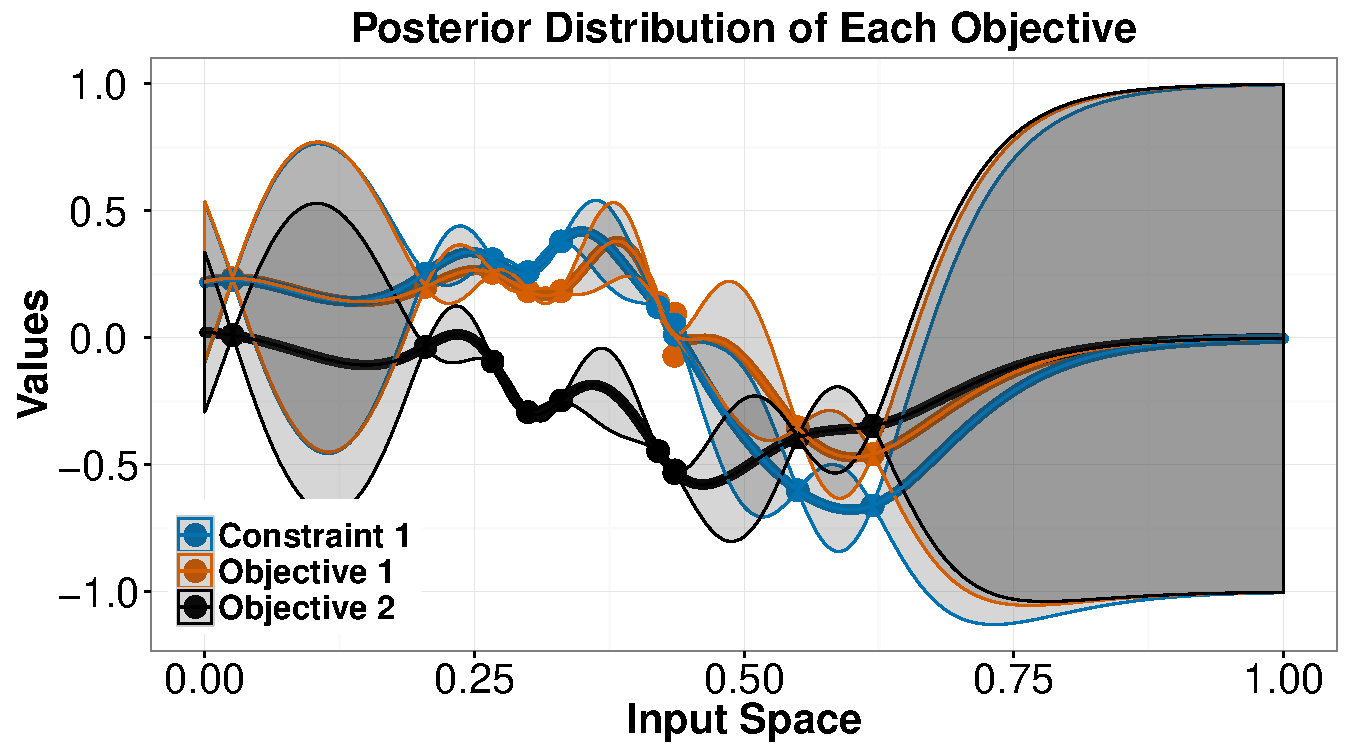
\includegraphics[width=0.7\linewidth]{figures/acquisition/plot_posterior_coupled.pdf} \\
        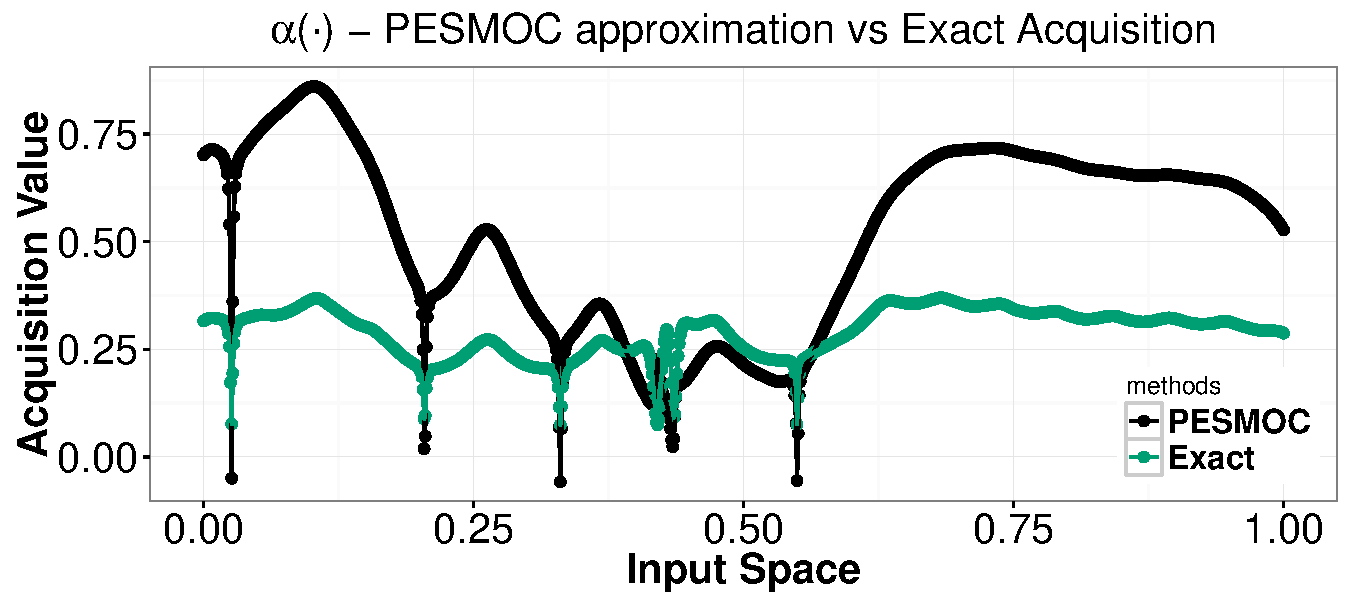
\includegraphics[width=0.7\linewidth]{figures/acquisition/plot_acq_coupled.pdf}
\end{tabular}
\caption{(top) Posterior distribution of each black-box function 
	(mean and standard deviation). (bottom) Acquisition function estimated by PESMOC and by a more expensive 
	but accurate Monte Carlo method combined with a non-parametric estimator of the entropy (exact). 
	}
        \label{fig:exact_coupled}
\end{center}
\end{figure}

We repeat these experiments in a decoupled scenario in which the different black-boxes need not be evaluated
at the same input location. The results are displayed in Figure \ref{fig:exact_decoupled}. In this case, we
show the estimates of the acquisition function corresponding to each black-box function. Therefore,
there are three different acquisition functions displayed. The plots show 
again that the PESMOC's approximation is accurate w.r.t the exact acquisition function, as  estimated by the 
more expensive process described above. Again, each pair of estimates of the acquisition function for each 
black-box are heavily correlated, suggesting similar maximizers and often similar acquisition values. We 
believe that this results provides empirical evidence of the quality of the acquisition approximation carried out 
in the proposed method, PESMOC. The accuracy of this approximation is also validated by the good results 
obtained in the rest of the experiments described in this paper.

%DIF <  DHL: TODO cambiar la leyenda de la figura para que los nombres de las funciones de adquisición coincidan.
%DIF <  EGM: Done.
\DIFdelbegin %DIFDELCMD < 

%DIFDELCMD < %%%
\DIFdelend \begin{figure}[htb]
\begin{center}
\begin{tabular}{cc}
        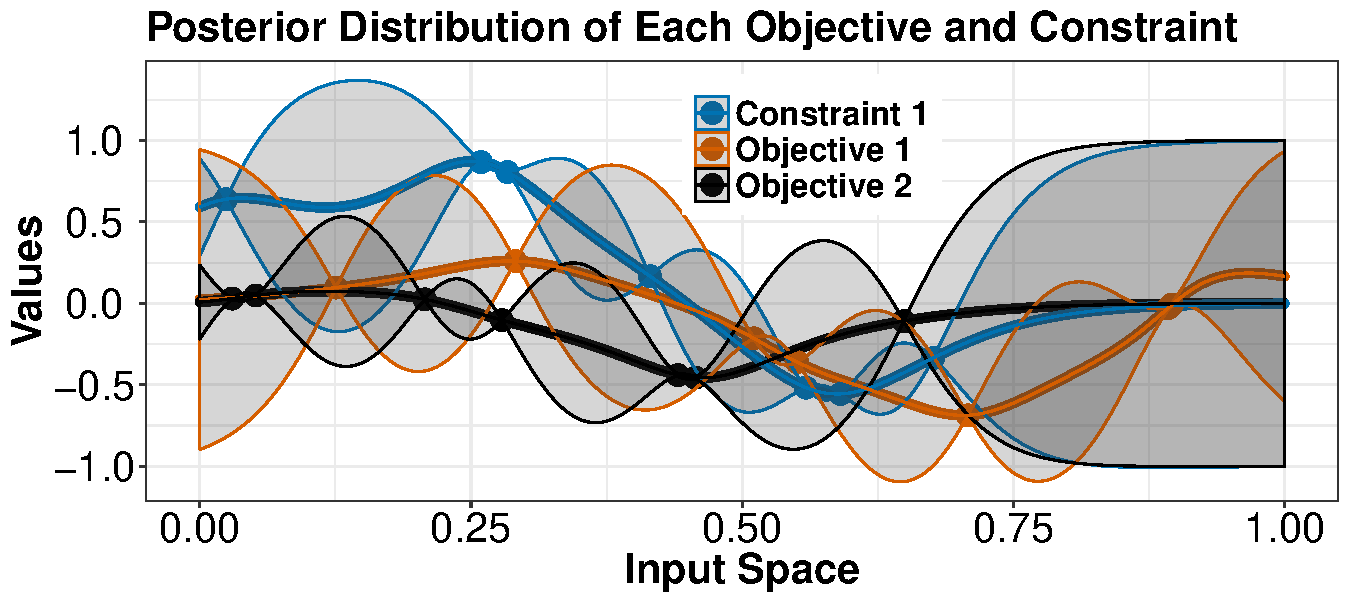
\includegraphics[width=0.45\linewidth]{figures/acquisition/plot_posterior.pdf} &
        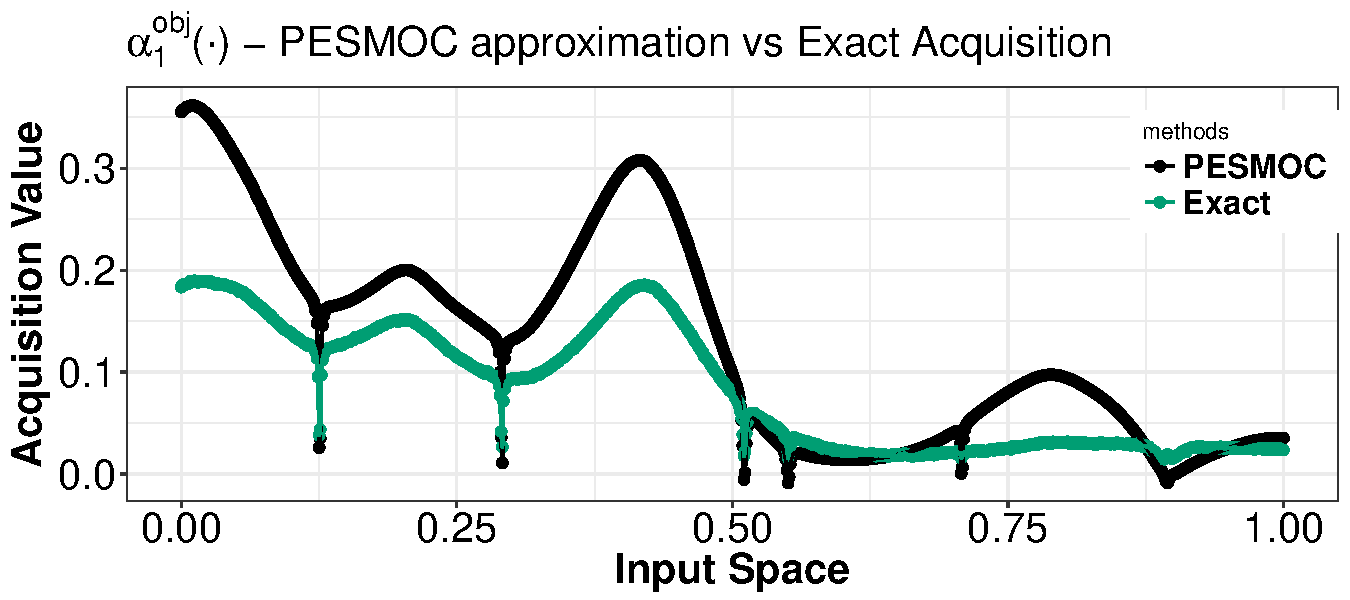
\includegraphics[width=0.45\linewidth]{figures/acquisition/plot_acq_obj_1.pdf} \\
        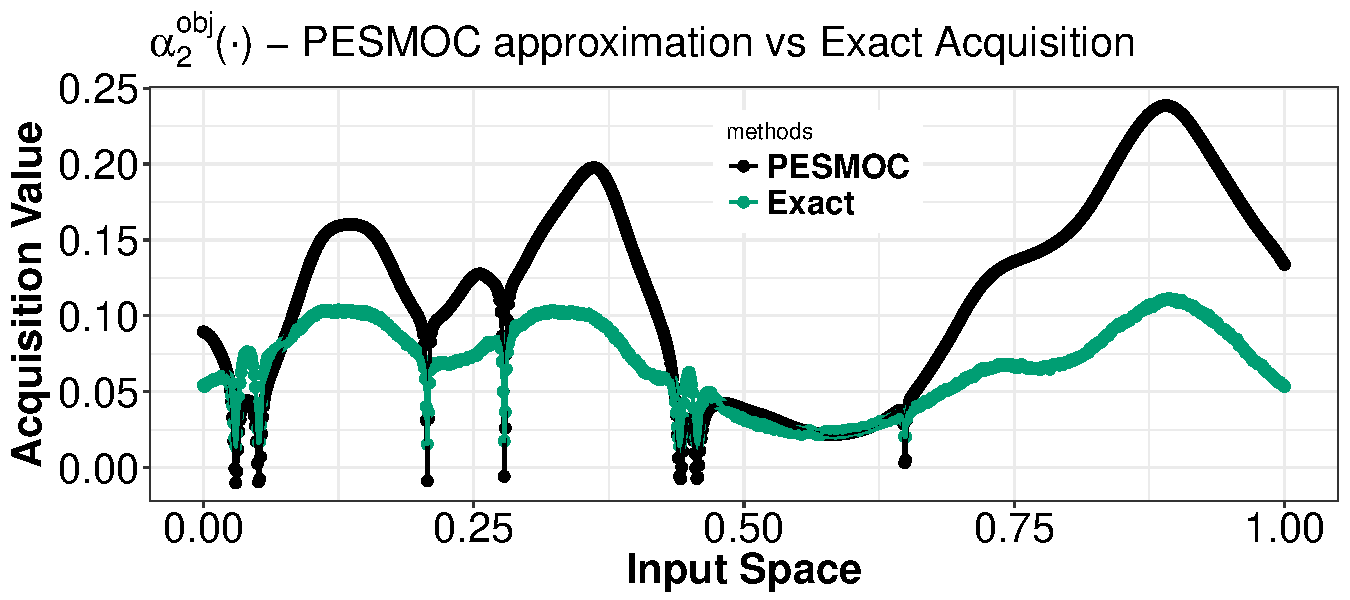
\includegraphics[width=0.45\linewidth]{figures/acquisition/plot_acq_obj_2.pdf} &
        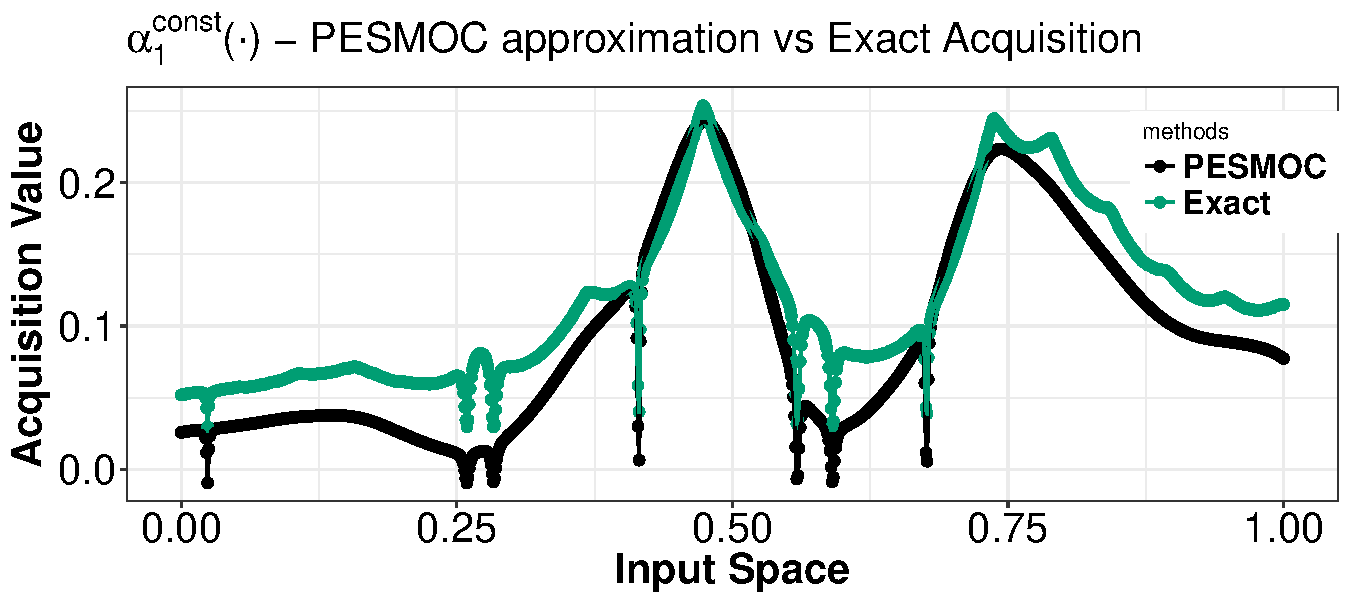
\includegraphics[width=0.45\linewidth]{figures/acquisition/plot_acq_con_1.pdf}
\end{tabular}
\caption{(top left) Posteriors distribution of each black-box function (mean and standard deviation).
	(top right to bottom right) Acquisition function for each black-box estimated by PESMOC and by a 
	more expensive but accurate Monte Carlo method combined with a non-parametric estimator of the entropy (exact). 
	}
        \label{fig:exact_decoupled}
\end{center}
\end{figure}

%DIF > Given the number of approximations performed, we can not provide theoretical hints of the quality of the approximation function
%DIF > but we do empirically provide strong arguments for the validity of the approximation not only in this work but also in previous works
%DIF > on this approximation \citep{hernandez2014predictive} \citep{hernandez2015predictive}. In particular, in addition to the described
%DIF > experiment of this section, we provide, in the supplementary material, an analysis of the impact of considering a variable number of Pareto Set points and number of Montecarlo iterations, showing that we obtain good results for given values of these hyperparameters that are involved
%DIF > in the approximation of PESMOC. The expectation propagation algorithm \citep{minka2001expectation} involved in the PESMOC approximation has been studied to be a valid methodology for variational inference \citep{seeger2005expectation}. We provide in further sections more empirical evidence to support our claim in the form of synthetic, benchmark and real experiments.
\DIFaddbegin 

\DIFaddend \subsection{Synthetic Experiments}

We compare the performance of PESMOC and BMOO with that of a random search strategy when the objectives and 
constraints are sampled from a GP prior. For this, we generate 100 optimization problems involving 2 objectives 
and 2 constraints in a 4-dimensional input space. This experiment is repeated to consider a more complicated setting.
In this case, we generate 100 optimization problems involving 4 objectives and 2 constraints in a 6-dimensional input 
space.  Each strategy (PESMOC, PESMOC decoupled, BMOO and Random) is run on each problem until 100 evaluations of each 
black-box are made. We report results for a noiseless and noisy evaluation scenario, in which we observe the evaluations 
are contaminated with additive Gaussian noise with standard deviation equal to $0.1$.  After each iteration of the optimization
process, each strategy outputs a recommendation in the form of a Pareto set obtained by optimizing the posterior means of the GPs,
as indicated at the beginning of this section. The performance criterion used is the hyper-volume of the corresponding 
solution. Recall that  the hyper-volume is the volume of points in functional space above the optimal points contained
in the recommendation. This quantity is maximized by the actual Pareto set \citep{zitzler1999multiobjective}. 
In the case that the recommendation produced contains an infeasible point, we 
simply set the hyper-volume of the recommendation equal to zero. For each method evaluated we report the logarithm of 
the relative difference between the hyper-volume of the actual Pareto set and the hyper-volume of the recommendation. 

\begin{figure}[htb]
\begin{tabular}{cc}
	\vspace{-.2cm}
	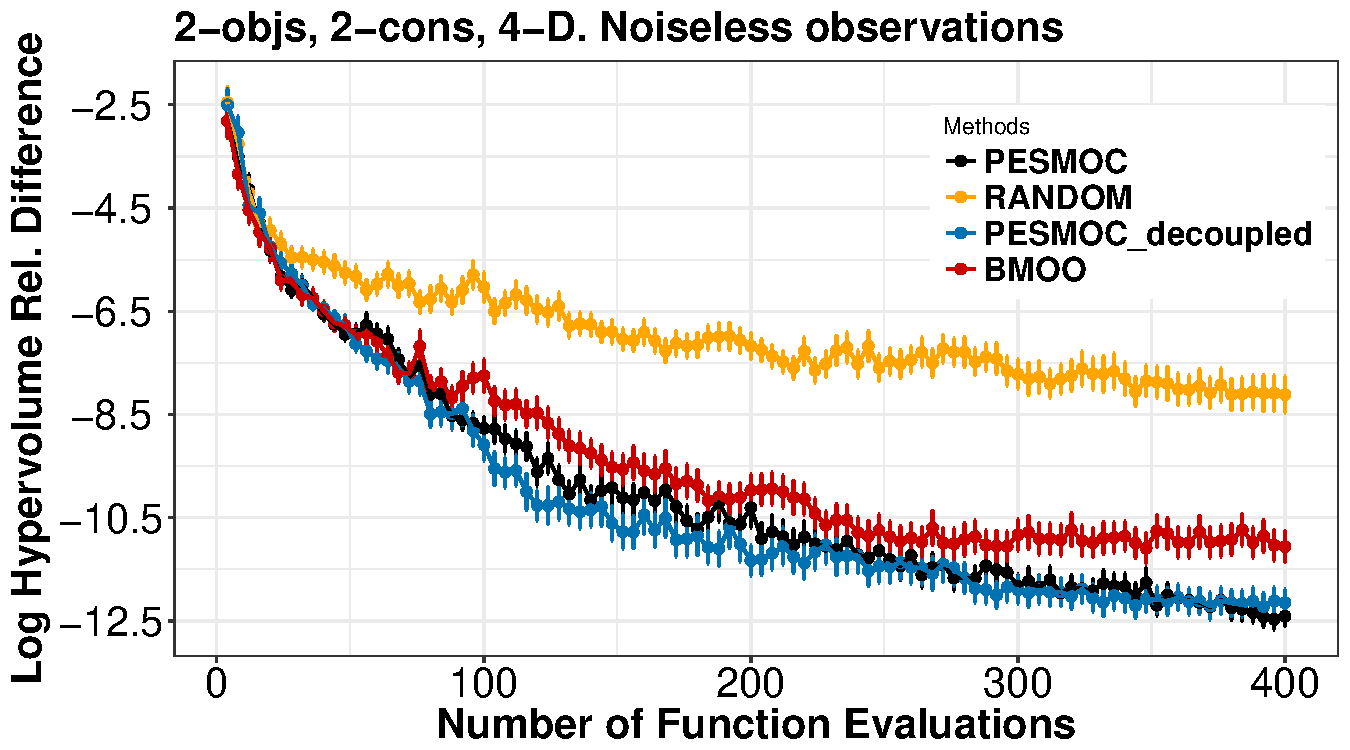
\includegraphics[width=0.475\linewidth]{figures/synthetic/4d_noiseless_NEW.pdf} &
	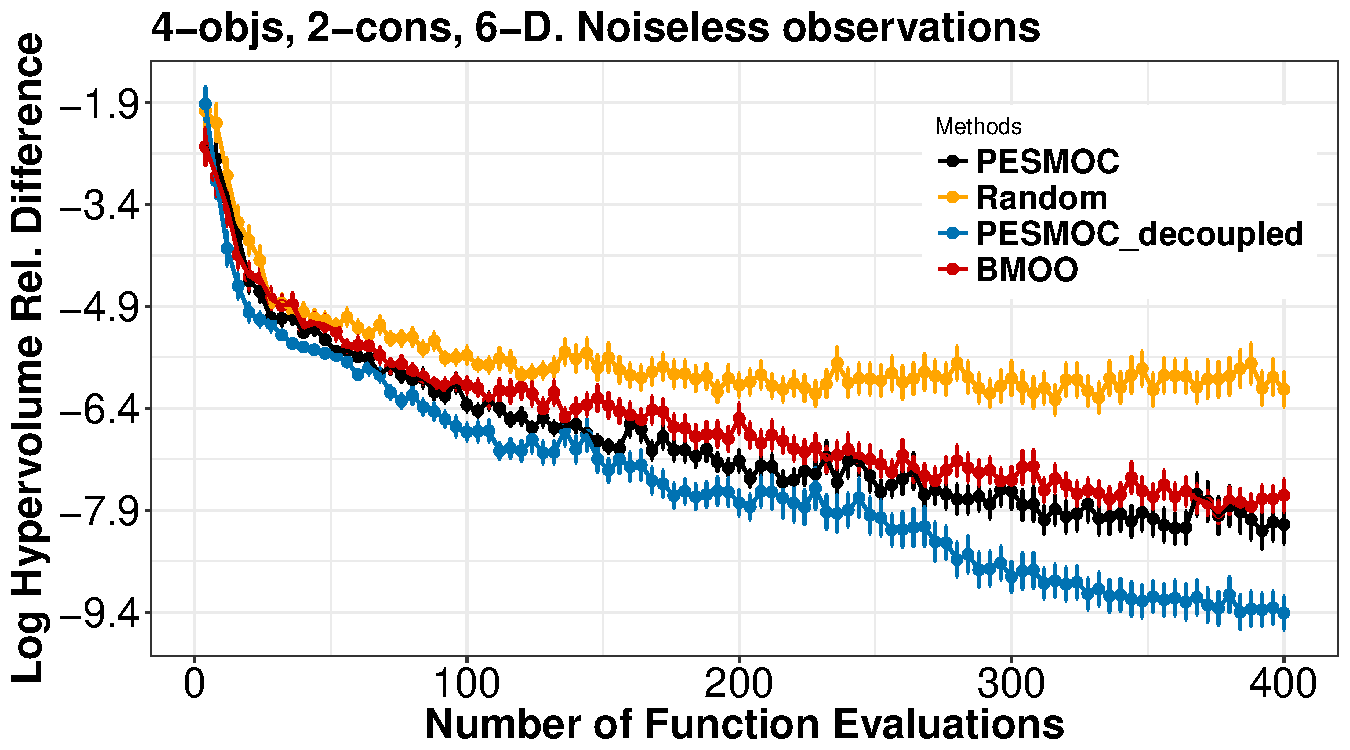
\includegraphics[width=0.475\linewidth]{figures/synthetic/6d_noiseless_NEW.pdf} \\\\
	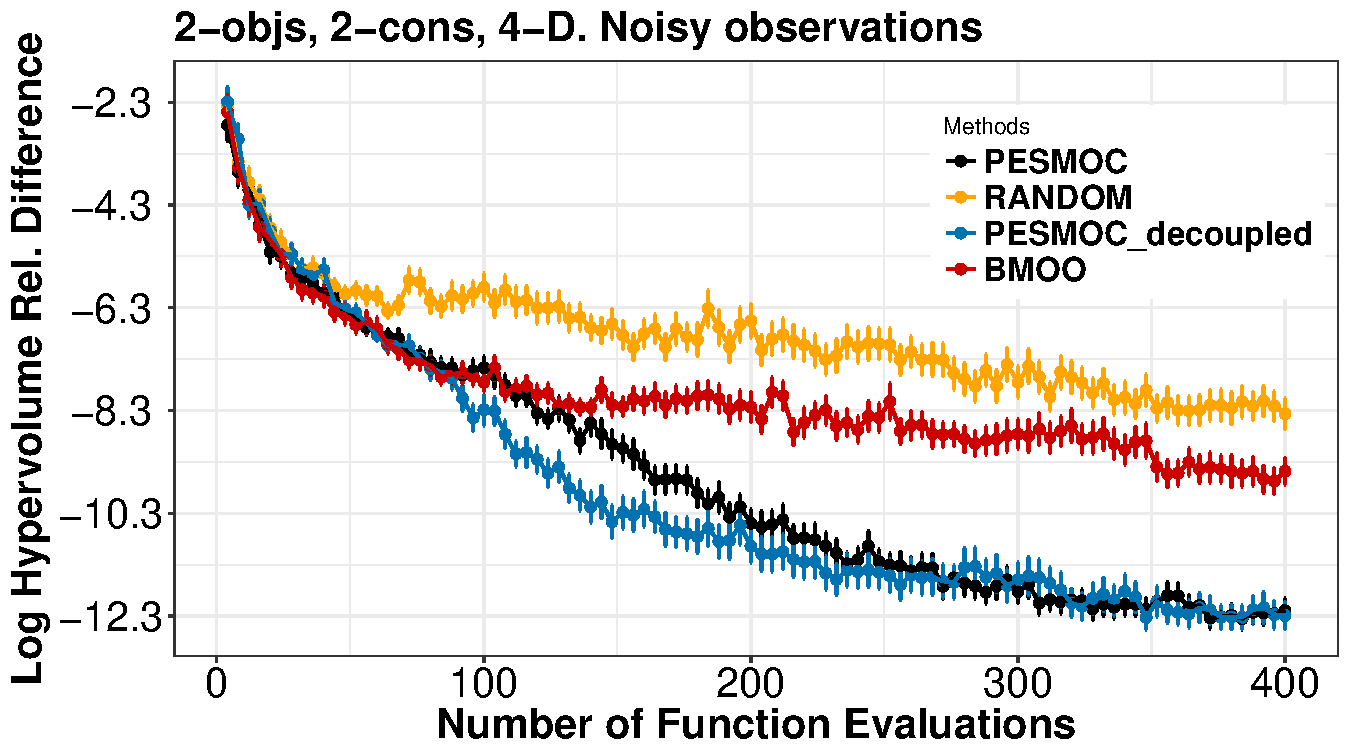
\includegraphics[width=0.475\linewidth]{figures/synthetic/4d_noisy_NEW.pdf} &
        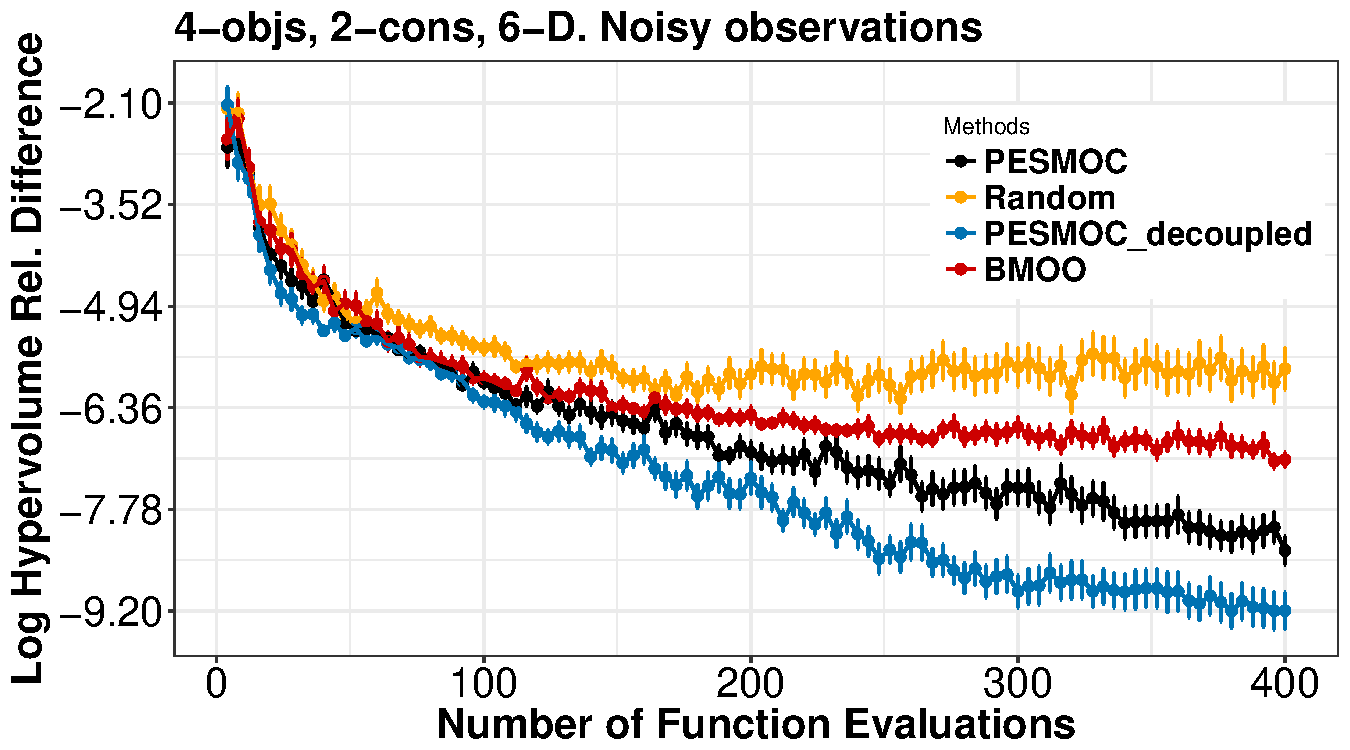
\includegraphics[width=0.475\linewidth]{figures/synthetic/6d_noisy_NEW.pdf}
	\vspace{-.1cm}
\end{tabular}
\caption{{\small Logarithm of the relative difference between the hyper-volume of 
the recommendation obtained by each method and the hyper-volume of the actual solution. 
We report results after each evaluation of the black-box functions. (left column) Two objectives and two constraints. 
Input space of four dimensions ($d=4$). (right column) 
Four objectives and two constraints.  Input space of six dimensions ($d=6$). (top row) 
Noiseless evaluation scenario. (bottom row) Noisy evaluation scenario. Best seen in color.}}
	\label{fig:results_synthetic}
	\vspace{-.25cm}
\end{figure}

Figure \ref{fig:results_synthetic} shows the average results obtained for each method and the corresponding error bars.
We observe that the PESMOC approaches outperform both BMOO and the random search approach in the two settings considered. 
In particular, PESMOC is able to find better solutions to the optimization problems considered, which are more accurate than 
those obtained by the other methods. These solutions have a hyper-volume that is closer to the hyper-volume of the actual Pareto set.
The random search method is also outperformed by BMOO in the two settings considered. However, BMOO gives worse results 
in the noisy scenario, as it tends to provide results that are closer to this method. Importantly, 
the decoupled version of PESMOC is similar or even better than the corresponding coupled counterpart. When the input 
dimension $d$ grows the improvements become evident. These results confirm the benefits of a decoupled evaluation 
setting. In particular, the decoupled version of PESMOC is the best overall method, significantly outperforming all 
other approach in the $6$-dimensional setting.


We also compare here the average time used by each strategy to choose the next evaluation. For this, we consider 
the synthetic experiments that involves 2 objectives  and 2 constraints, in a 4-dimensional input space, with noisy 
evaluations, and the experiment that involves 4 objectives, 2 constraints and a 6-dimensional input space, not considering noise.
For each method and each iteration, we measure the average time spent in the computation and 
maximization of the acquisition function. In the case of PESMOC this time includes the time required to run EP until convergence, 
and the time required to optimize the acquisition function. In the case of BMOO this time includes the time required
to generate the Monte Carlo samples used in (\ref{eq:acc_bmoo}) to approximate the acquisition function, and the time required 
for its optimization. The results obtained are shown in Table \ref{table:times}. We do not include in this table
the random search strategy, since the time it requires to choose the next evaluation is negligible.

\begin{table}[htb]
\centering
\caption{Average time in seconds spent on each iteration by each method. First row corresponds to the 4-dimensional input space experiment and the second row corresponds to the 6-dimensional input space experiment.}
{\small
\begin{tabular}{c|c | c | c}
 \hline
 \bf{Experiment} & {\bf PESMOC coupled} & {\bf PESMOC decoupled} & {\bf BMOO}\\
 \hline
 First & $41.40 \pm 1.48$ & $49.63 \pm 1.02$ & $67.41 \pm 4.29$\\
 Second & $112.94 \pm 3.25$ & $264.60 \pm 3.36$ & $307.90 \pm 34.00$\\
 \hline
\end{tabular}
}
\label{table:times}
\end{table}

Table \ref{table:times} shows that the fastest strategy is PESMOC, followed by the decoupled version of PESMOC and BMOO. BMOO is significantly slower 
than PESMOC, due to the need of running the Metropolis-Hastings algorithm.  By constrast, in PESMOC, EP converges in just a few iterations. Note that 
the decoupled version of PESMOC is slightly slower than the coupled counterpart per iteration.  The reason is that it requires the optimization of one acquisition 
function per each black-box function, to determine the next evaluation, instead of just one as in the PESMOC case. Note that this only represents a 
small fraction of the total time per iteration of PESMOC in the decoupled setting (the time of fitting the GPs and running the EP algorithm to approximate the 
factors that do not depend on the candidate point $\mathbf{x}$ is similar for the coupled and the decoupled setting). Importantly, however, 
the decoupled version will need as many more iterations as black boxes are present in the problem. For example, in the first problem, which has 4 black-box functions, 
to perform 400 evaluations of the black-boxes, the coupled version of PESMOC will require 100 iterations, while the decoupled version will require 400. The results 
shown in the table are expected to generalize to other problems involving a different number of black-boxes or input dimensions.

We also illustrate here the shape of the acquisition function of PESMOC on a toy 2-dimensional optimization 
problem with input domain $\mathcal{X}$ given by the box $[-10,10]\times[-10,10]$:
\begin{align}
\underset{\mathbf{x} \in \mathcal{X}}{\text{min}} & \quad f_1(x,y) = xy, 
\quad f_2(x,y) = -yx \nonumber \quad \text{s.t.} \quad x \geq 0, y \geq 0\,.
\end{align}
In this experiment the feasible space $\mathcal{F}$ is given by the box $[0,10]\times[0,10]$. 
Figure \ref{fig:evaluations} shows the location of the first 20 evaluations made
by each method (blue crosses) and the level curves of the acquisition function of PESMOC and BMOO. 
We observe that PESMOC and BMOO quickly identify the feasible space $\mathcal{F}$, and focus on 
evaluating the black-box functions in that region. By contrast, the random search strategy explores the space 
more uniformly and evaluates the black-boxes more frequently in regions of the input space that are infeasible. 
We observe that the acquisition functions of PESMOC and BMOO take high values inside 
$\mathcal{F}$ and low values outside $\mathcal{F}$.

\begin{figure}[htb]
	\begin{tabular}{cc}
	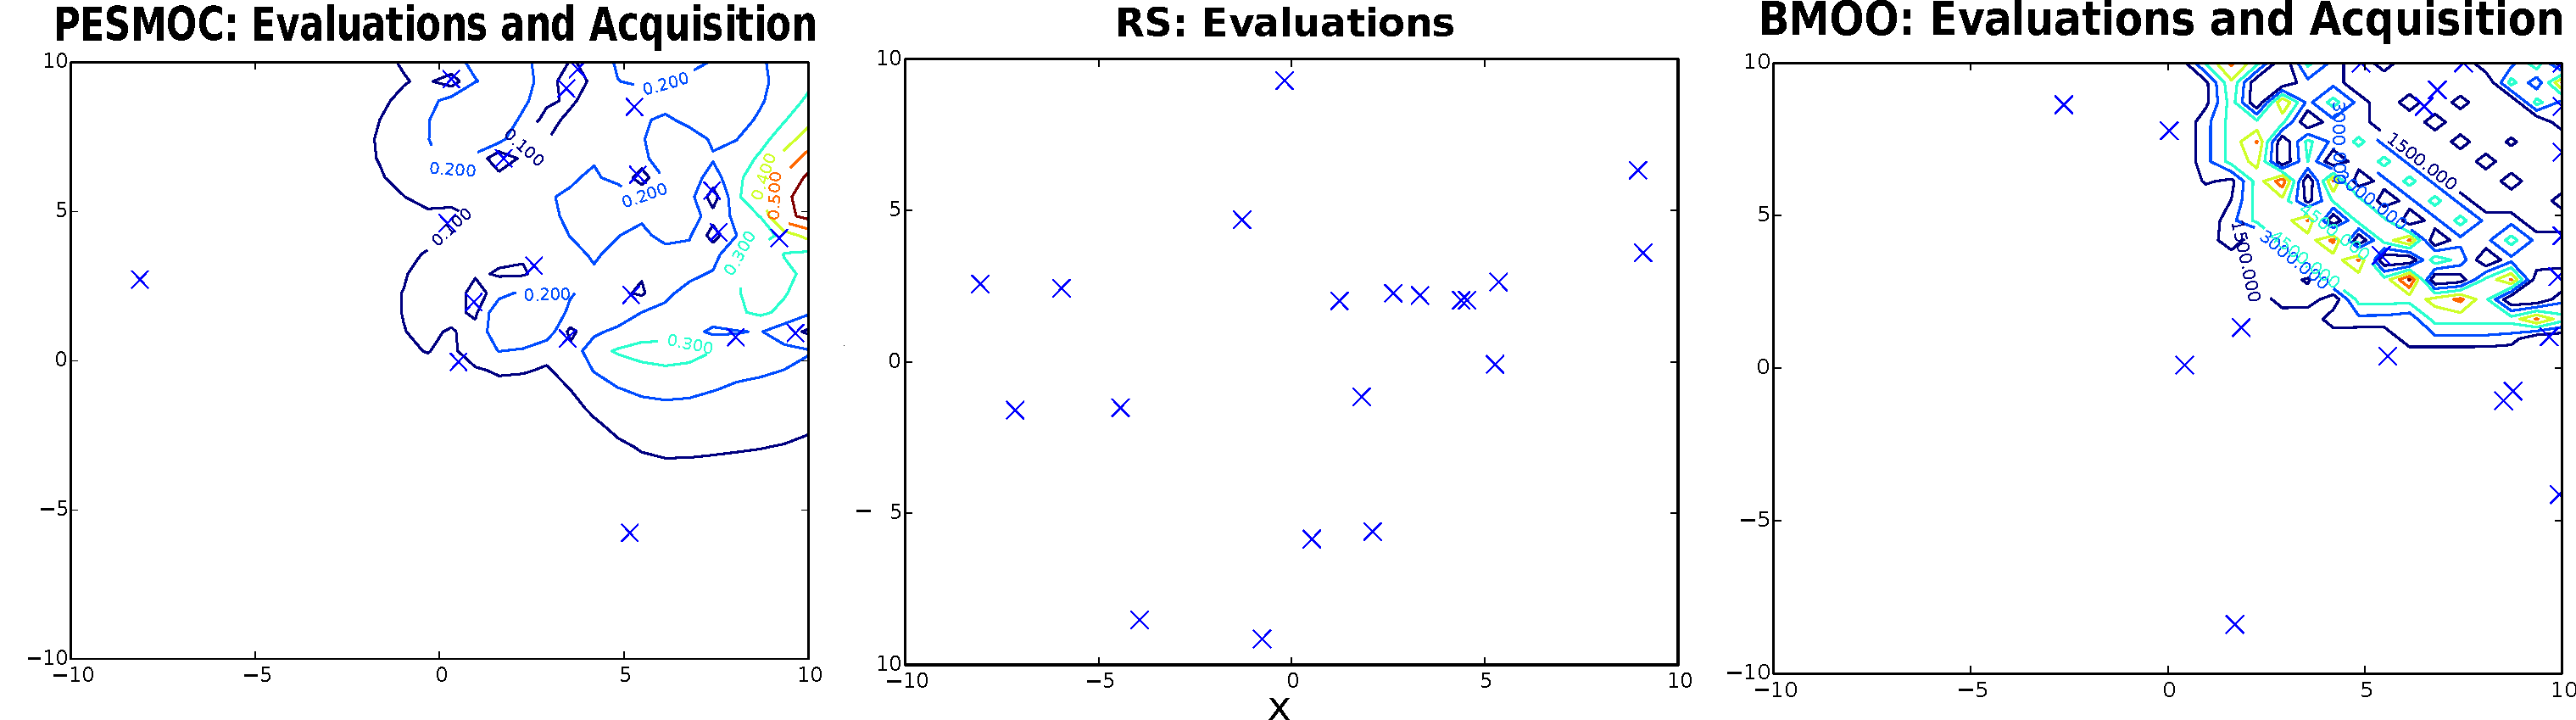
\includegraphics[width=0.9\linewidth]{figure.pdf}
	%\includegraphics[width=0.32\linewidth]{20-acq.pdf} &
	%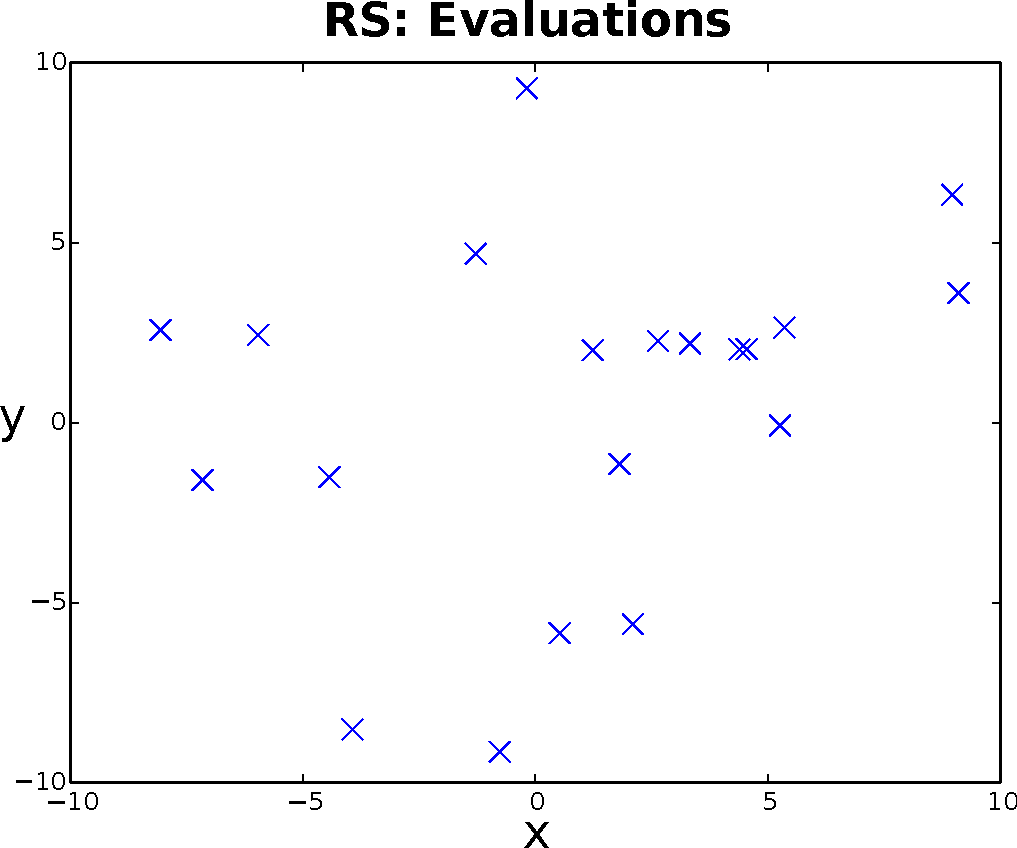
\includegraphics[width=0.3\linewidth]{20-mocotoy_1-observations.pdf}
	%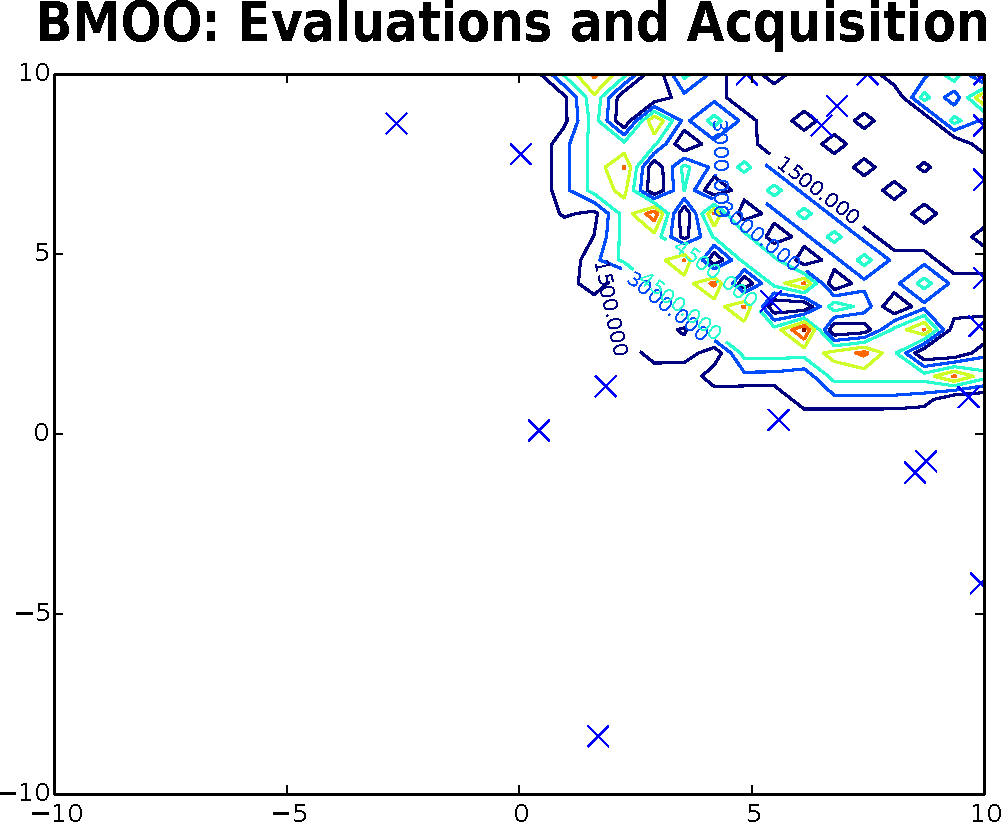
\includegraphics[width=0.3\linewidth]{20-acq-bmoo.pdf}
	\end{tabular}
	\caption{{\small Location in input space (denoted with a blue cross) of each of the evaluations made by PESMOC 
		(left), random search (middle) and BMOO (right). In the case of PESMOC and BMOO, we also plot the level 
		curves of the acquisition function. The feasible region is the the box $[0,10] \times [0,10]$. Best seen in color. }}
	\label{fig:evaluations}
\end{figure}

\subsection{Benchmark Experiments}

In the previous experiments the black-boxes are sampled from a GP prior, which is the underlying model assumed by the different
BO methods compared. This hypothesis need not be satisfied in practice. Therefore, model misspecification may have an impact in 
the performance of BO methods. In this section we carry out extra experiments with the goal of comparing the different methods 
under such a scenario. For this, we consider 7 classical benchmark problems used to assess multi-objective optimization methods 
with constraints \citep{chafekar2003constrained,deb2002fast}. A summary of these problems is displayed in Table \ref{table:1} and \ref{table:1_b}. 
All problems contain several input variables, multiple objectives and several constraints. Importantly, in these experiments 
we transform each constraint $c_j(\mathbf{x})$ so that the corresponding optimization problem can be expressed as 
in (\ref{eq:optimization}). Furthermore, we also consider a noiseless and a noisy setting, in which the evaluations of the
black-boxes are contaminated with additive Gaussian noise. The variance of the noise is set to 1\% of the range of potential 
values of the corresponding black-box. This range of values is found by evaluating each black-box function on a grid.
These experiments are repeated 100 times for each method and each dataset and we report average results. The metric used
to assess the performance of each method is the same as the one employed in the previous section.

\begin{table}[H]
\centering
\caption{Summary of BNH, SRN, TNK and OSY problems used in the benchmark experiments.}
{\small
\begin{tabular}{| c | c | c |}
 \hline
 \multicolumn{3}{|c|}{Benchmark Experiments} \\
 \hline
 Problem Name & Input Space & Objectives $f_k(\mathbf{x})$ and Constraints $c_j(\mathbf{x})$ \\
 \hline
 \multirow{4}{4em}{BNH} & \multirow{4}{7em}{$x_1 \in [0,5]$\\$x_2 \in [0,3]$} & $f_1(\mathbf{x}) = 4x_1^2 + 4x_2^2$ \\ 
 & & $f_2(\mathbf{x}) = (x_1-5)^2 + (x_2-5)^2$ \\  
 & & $c_1(\mathbf{x}) \equiv (x_1-5)^2 + x_2^2 \leq 25$ \\ 
 & & $c_2(\mathbf{x}) \equiv (x_1-8)^2 + (x_2+3)^2 \geq 7.7$ \\ 
 \hline 
 \multirow{4}{4em}{SRN} & \multirow{4}{7em}{$x_1 \in [-20,20]$\\$x_2 \in [-20,20]$} & $f_1(\mathbf{x}) = 2+(x_1-2)^2+(x_2-2)^2$ \\
 & & $f_2(\mathbf{x}) = 9x_1 - (x_2-1)^2$ \\
 & & $c_1(\mathbf{x}) \equiv x_1^2 + x_2^2 \leq 225$ \\
 & & $c_2(\mathbf{x}) \equiv x_1 - 3x_2 + 10 \leq 0$ \\
 \hline
 \multirow{4}{4em}{TNK} & \multirow{4}{7em}{$x_1 \in [0,\pi]$\\$x_2 \in [0,\pi]$} & $f_1(\mathbf{x}) = x_1$ \\
 & & $f_2(\mathbf{x}) = x_2$ \\
 & & $c_1(\mathbf{x}) \equiv x_1^2 + x_2^2 - 1 - 0.1 cos(16arctan\frac{x_1}{x_2}) \geq 0$ \\
 & & $c_2(\mathbf{x}) \equiv (x_1-0.5)^2 + (x_2-0.5)^2 \leq 0.5$ \\
 \hline
\multirow{9}{4em}{OSY} & \multirow{9}{7em}{$x_1 \in [0,10]$\\$x_2 \in [0,10]$\\$x_3 \in [1,5]$\\$x_4 \in [0,6]$\\$x_5 \in [1,5]$\\$x_6 \in [0,10]$} & 
$f_1(\mathbf{x}) = -[25(x_1-2)^2+(x_2-2)^2+(x_3-1)^2$ \\
 & &  $+(x_4-4)^2+(x_5-1)^2$ \\
 & & $f_2(\mathbf{x}) = x_1^2+x_2^2+x_3^2+x_4^2+x_5^2+x_6^2$ \\
 & & $c_1(\mathbf{x}) \equiv x_1+x_2-2 \geq 0$ \\
 & & $c_2(\mathbf{x}) \equiv 6-x_1-x_2 \geq 0$ \\
 & & $c_3(\mathbf{x}) \equiv 2-x_2+x_1 \geq 0$ \\
 & & $c_4(\mathbf{x}) \equiv 2-x_1+3x_2 \geq 0$ \\
 & & $c_5(\mathbf{x}) \equiv 4-(x_3-3)^2-x_4 \geq 0$ \\
 & & $c_6(\mathbf{x}) \equiv (x_5-3)^2+x_6-4 \geq 0$ \\
 \hline
\end{tabular}
}
\label{table:1}
\end{table}
\begin{table}[H]
\centering
\caption{Summary of CONSTR, Two-bar Truss and Welded Beam problems used in the benchmark experiments.}
{\small
\begin{tabular}{| c | c | c |}
 \hline
 \multicolumn{3}{|c|}{Benchmark Experiments} \\
 \hline
 Problem Name & Input Space & Objectives $f_k(\mathbf{x})$ and Constraints $c_j(\mathbf{x})$ \\
 \hline
 \multirow{4}{4em}{CONSTR} & \multirow{4}{7em}{$x_1 \in [0.1,10]$\\$x_2 \in [0,5]$} & $f_1(\mathbf{x}) = x_1$ \\
 & & $f_2(\mathbf{x}) = \frac{(1+x_2)}{x_1}$ \\
 & & $c_1(\mathbf{x}) \equiv x_2+9x_1 \geq 6$ \\
 & & $c_2(\mathbf{x}) \equiv -x_2+9x_1 \geq 1$ \\
 \hline
 \multirow{3}{4em}{Two-bar\\Truss\\Design} & \multirow{3}{7em}{$x_1 \in [0,0.01]$\\$x_2 \in [0,0.01]$\\$x_3 \in [1,3]$} & 
$f_1(\mathbf{x}) = x_1\sqrt{16+x_3^2} + x_2\sqrt{1+x_3^2}$ \\
 & & $f_2(\mathbf{x}) = \max(\frac{20\sqrt{16+x_3}}{x_1x_3},\frac{80\sqrt{1+x_3^2}}{x_2x_3})$ \\
 & & $c_1(\mathbf{x}) \equiv \max(\frac{20\sqrt{16+x_3}}{x_1x_3},\frac{80\sqrt{1+x_3^2}}{x_2x_3}) \leq 10^5$ \\
 \hline
\multirow{10}{4em}{Welded\\Beam\\Design} & \multirow{9}{7em}{$h \in [0.125,5]$\\$b \in [0.125,5]$\\$l \in [0.1,10]$\\$t \in [0.1,10]$} &   
$f_1(\mathbf{x}) = 1.10471h^2l + 0.04811tb(14+l)$ \\
 & & $f_2(\mathbf{x}) = \frac{2.1952}{t^3b}$ \\
 & & $c_1(\mathbf{x}) \equiv 13600-\tau(\mathbf{x}) \geq 0$ \\
 & & $c_2(\mathbf{x}) \equiv 30000-\frac{504000}{t^2b} \geq 0$ \\
 & & $c_3(\mathbf{x}) \equiv b-h \geq 0$ \\
 & & $c_4(\mathbf{x}) \equiv 64746.022(1-0.0282346t)tb^3-6000 \geq 0$ \\
 & & $\tau(\mathbf{x}) = \sqrt{\gamma(\mathbf{x})^2+\epsilon(\mathbf{x})^2+\frac{l\gamma(\mathbf{x})\epsilon(\mathbf{x})}{\sqrt{0.25(l^2+(h+t)^2)}}}$ \\
 & & $\gamma(\mathbf{x}) = \frac{6000}{\sqrt{2}hl}$ \\
 & & $\epsilon(\mathbf{x}) = \frac{6000(14+0.5l)\sqrt{0.25(l^2+(h+t)^2)}}{2\sqrt{2}hl(\frac{l^2}{12+0.25(h+t)^2})}$ \\
 \hline
\end{tabular}
}
\label{table:1_b}
\end{table}

Figure \ref{fig:benchmark_results_1} and \ref{fig:benchmark_results_2} show the average results of each method on these 
experiments with the corresponding error bars. In these experiments, when a particular method outputs an infeasible solution, 
(\emph{i.e.}, a solution that does not fulfil at least one of the constraints), that result is ignored. To guarantee a 
fair comparison, we have also recorded the fraction of times that an infeasible solution is returned by each method. 
If the performance of two methods is similar, it will be preferred the method that gives a lower percentage of 
infeasible solutions. In practice, we have observed that all the BO methods compared tend to provide a similar 
fraction of infeasible points. An exception is the random search strategy that systematically tends to recommend 
infeasible solutions. The complete results are found in the supplementary material.

\begin{figure}[H]
	\begin{tabular}{cc}
        	\vspace{-.2cm}
	        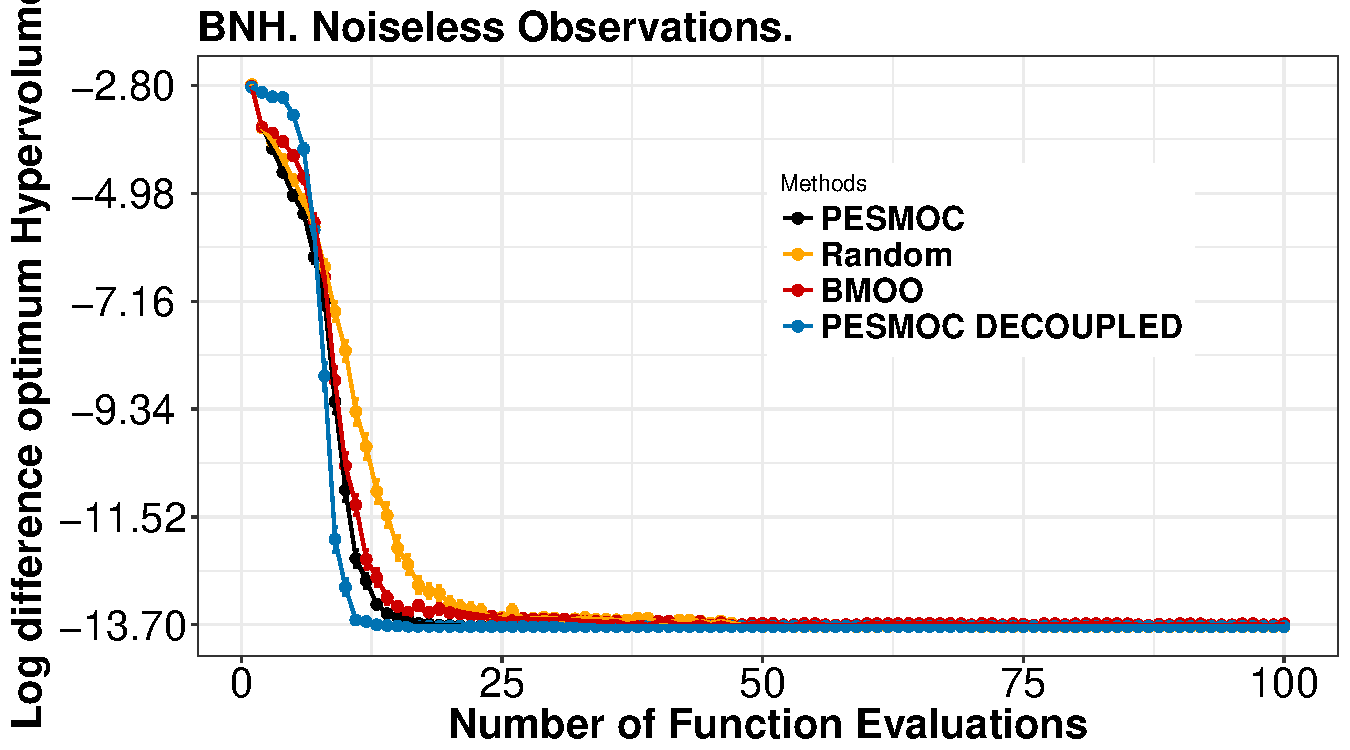
\includegraphics[width=0.475\linewidth]{figures/benchmark/BNH.pdf} &
	        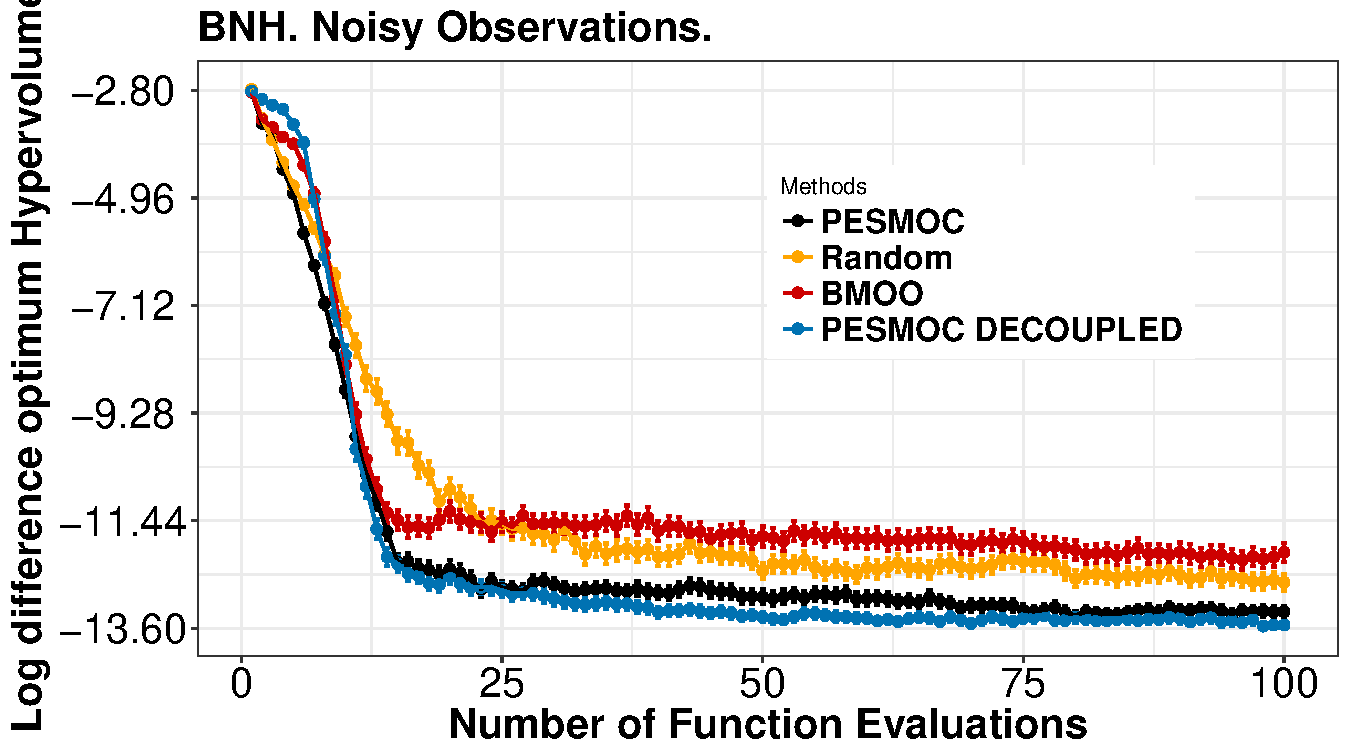
\includegraphics[width=0.475\linewidth]{figures/benchmark/BNH_noisy.pdf} \\
		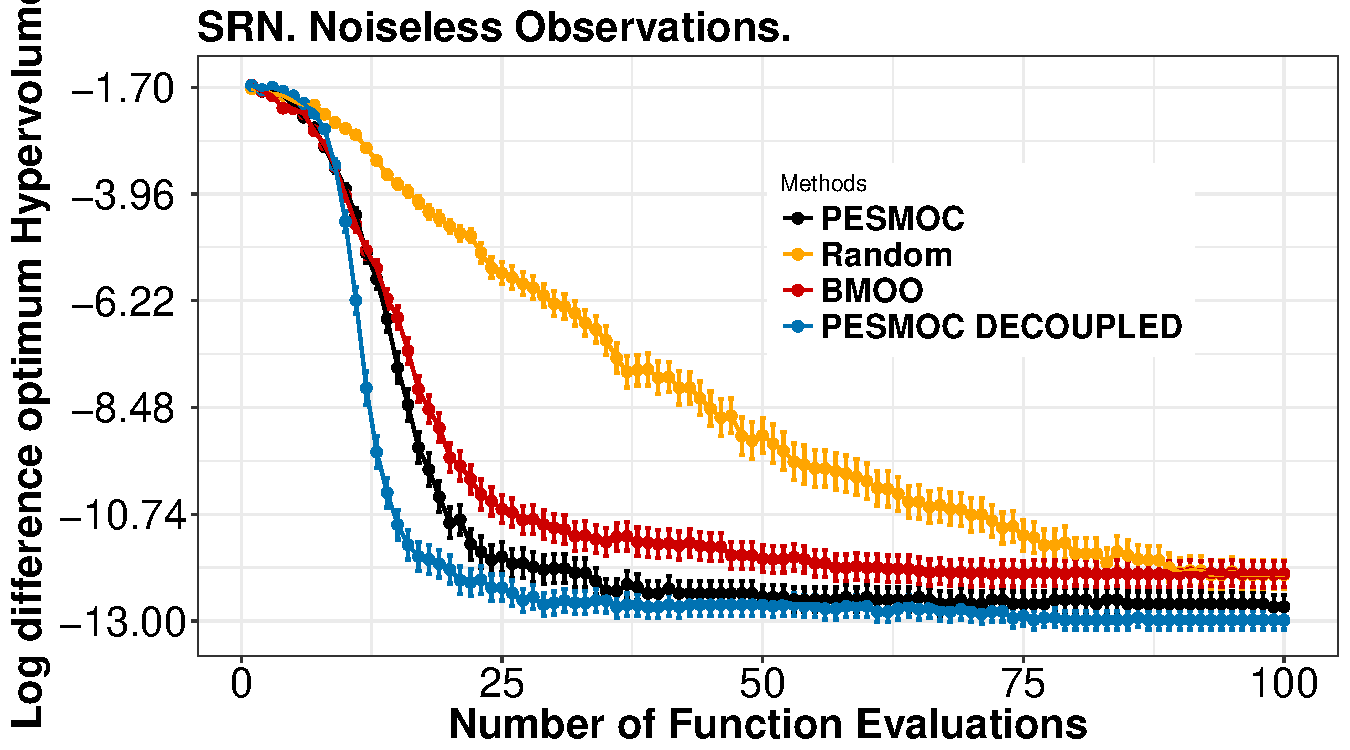
\includegraphics[width=0.475\linewidth]{figures/benchmark/SRN.pdf} &
                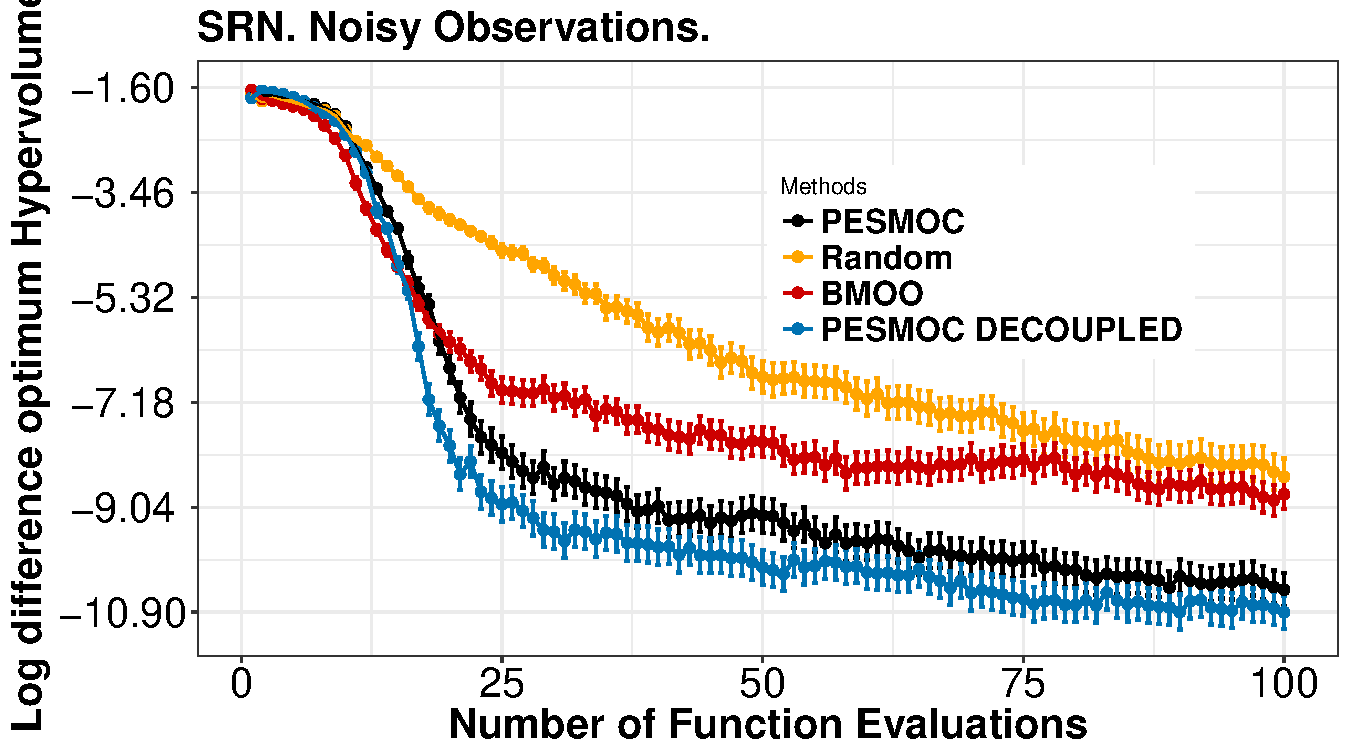
\includegraphics[width=0.475\linewidth]{figures/benchmark/SRN_noisy.pdf} \\
		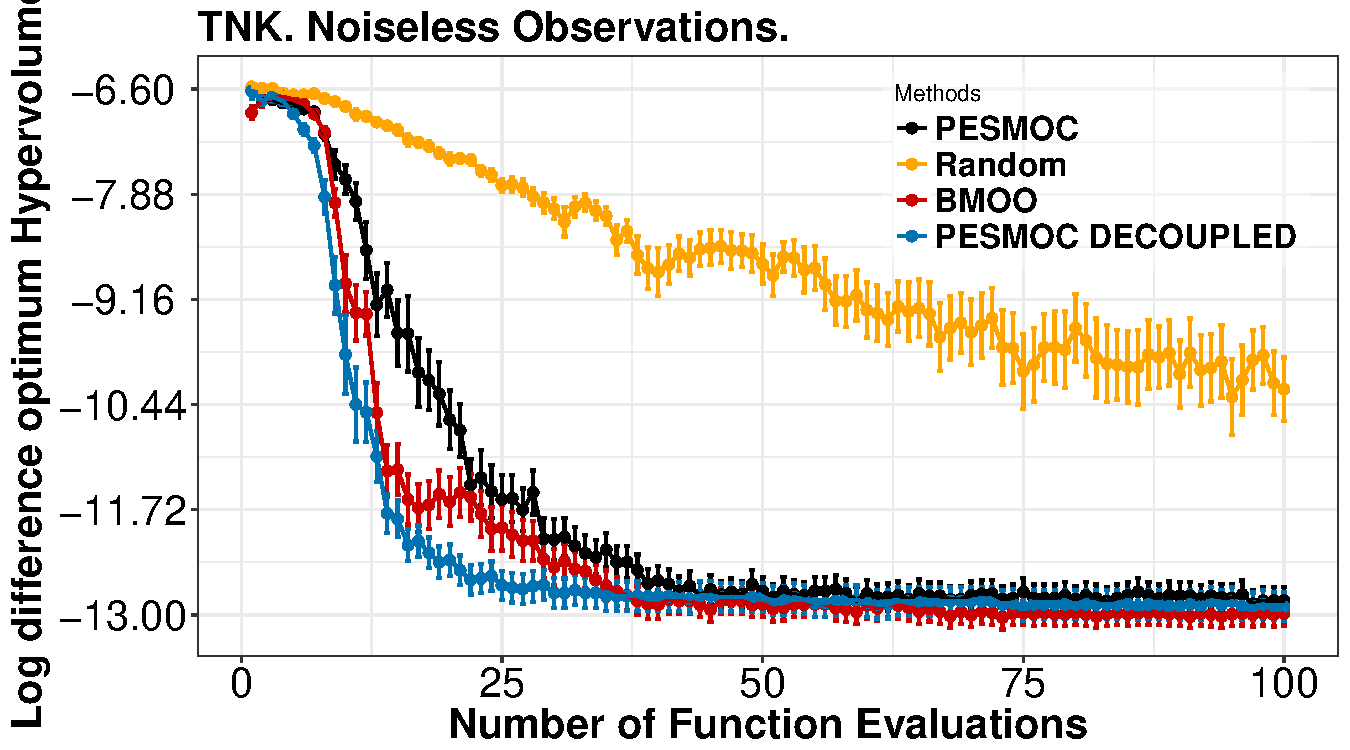
\includegraphics[width=0.475\linewidth]{figures/benchmark/TNK.pdf} &
                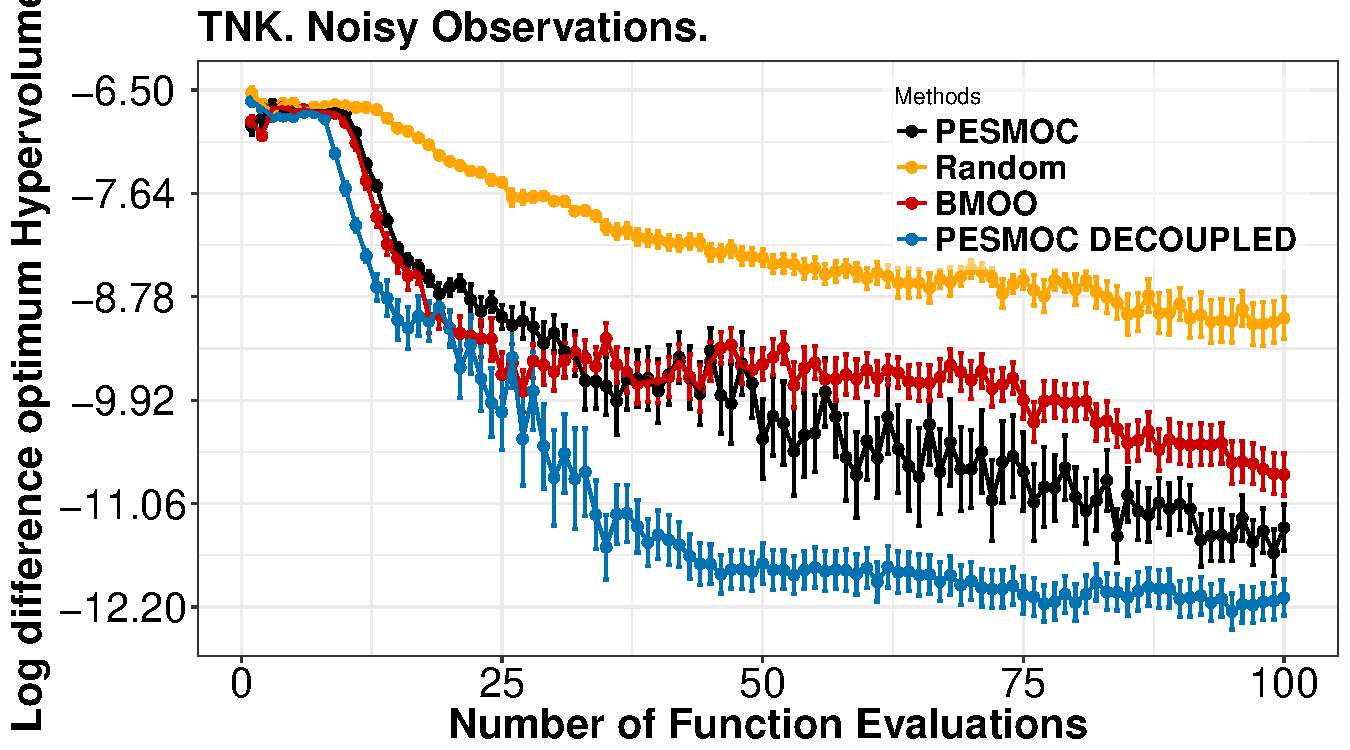
\includegraphics[width=0.475\linewidth]{figures/benchmark/TNK_noisy.pdf} \\
		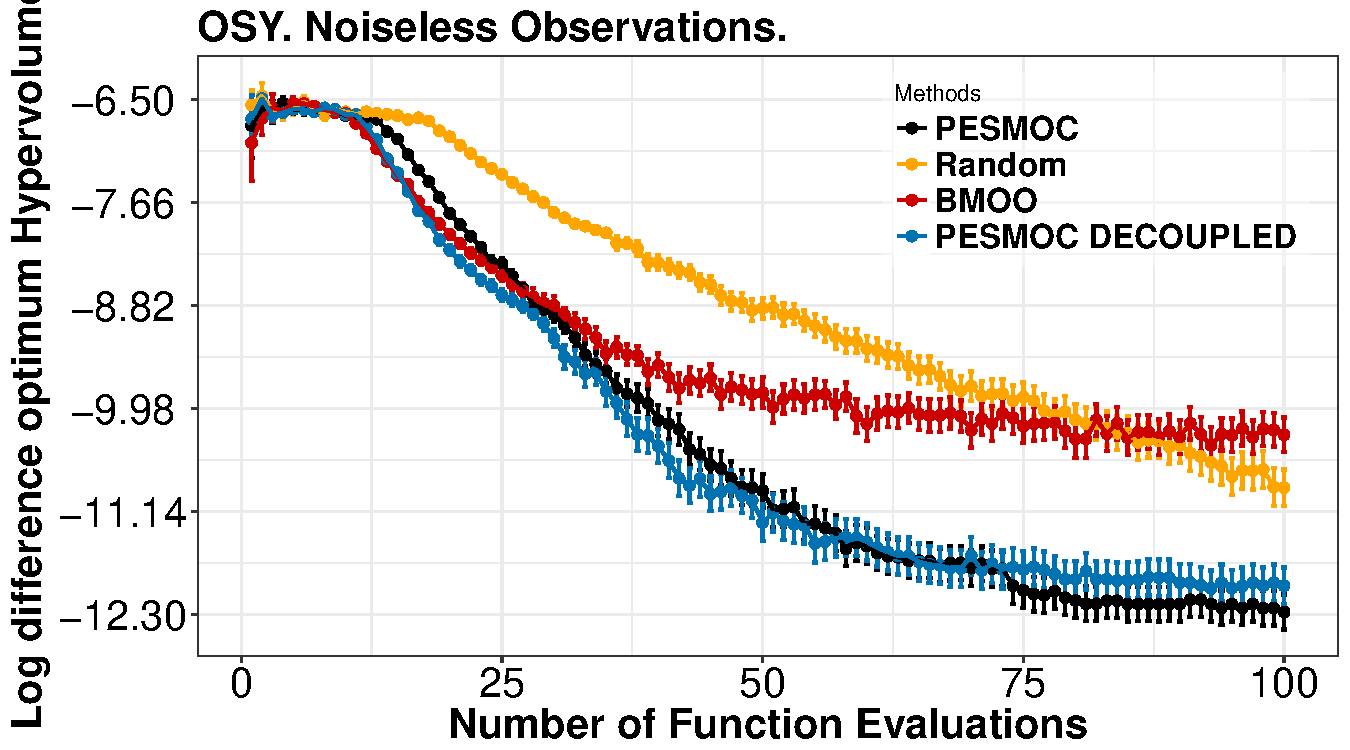
\includegraphics[width=0.475\linewidth]{figures/benchmark/OSY.pdf} &
                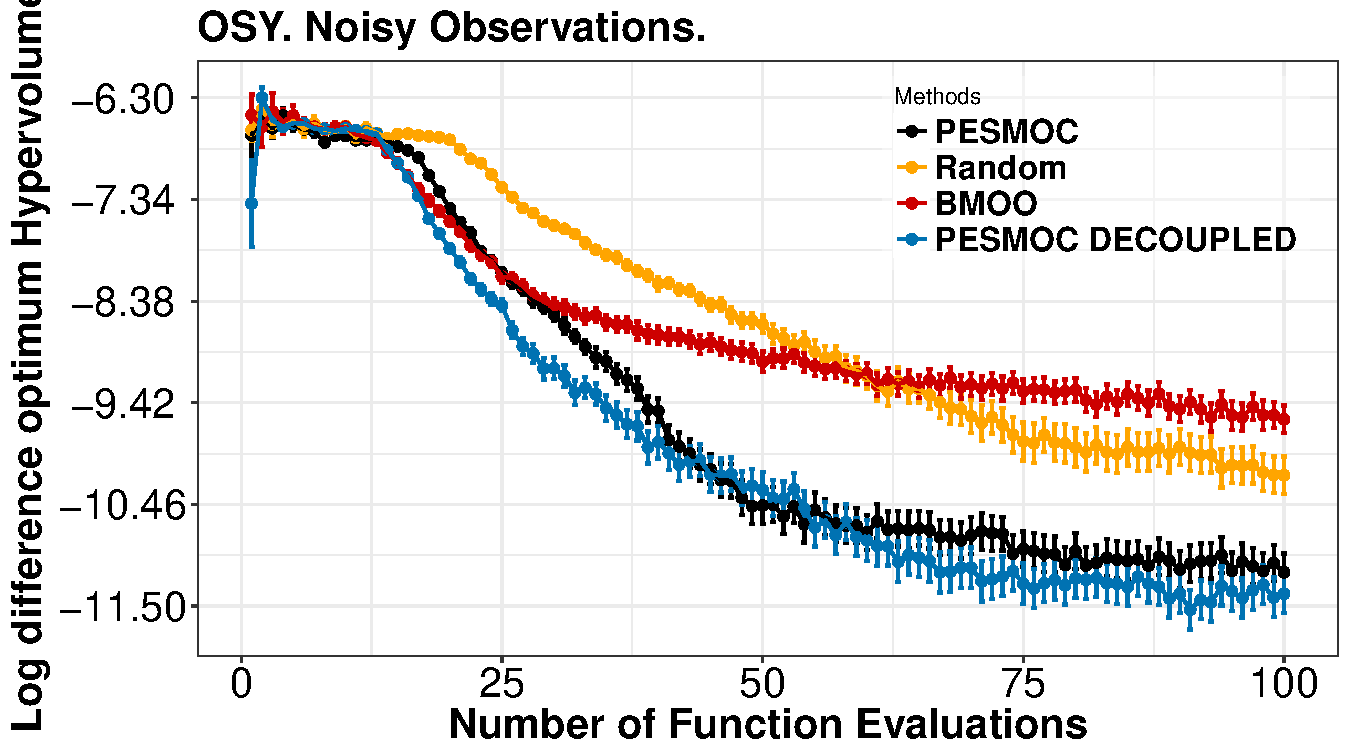
\includegraphics[width=0.475\linewidth]{figures/benchmark/OSY_noisy.pdf} \\
        \end{tabular}
        \caption{Results for the problems BNH, SRN, TNK and OSY. Noiseless and noisy settings. The plots show 
		the average log difference w.r.t to the optimal hyper-volume.} 
        \label{fig:benchmark_results_1}
\end{figure}

\begin{figure}[H]
        \begin{tabular}{cc}
                \vspace{-.2cm}
		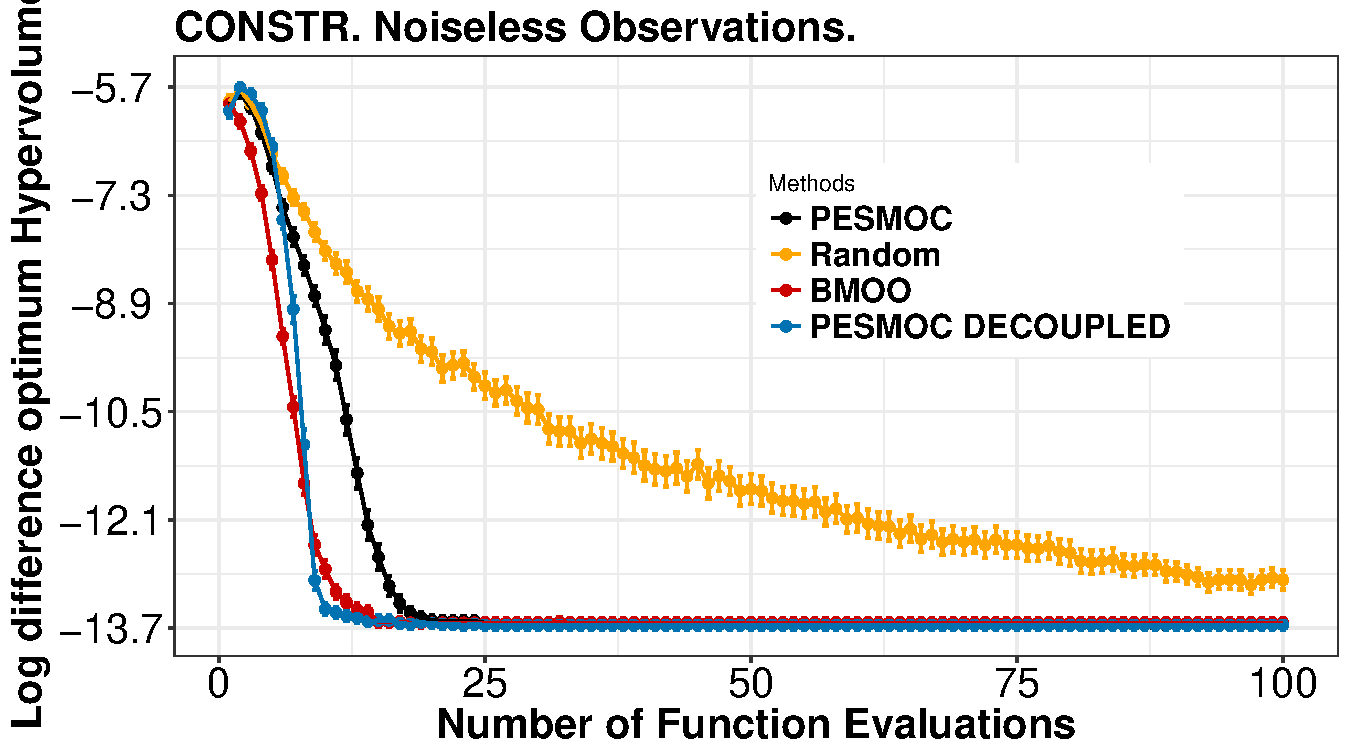
\includegraphics[width=0.475\linewidth]{figures/benchmark/CONSTR.pdf} &
                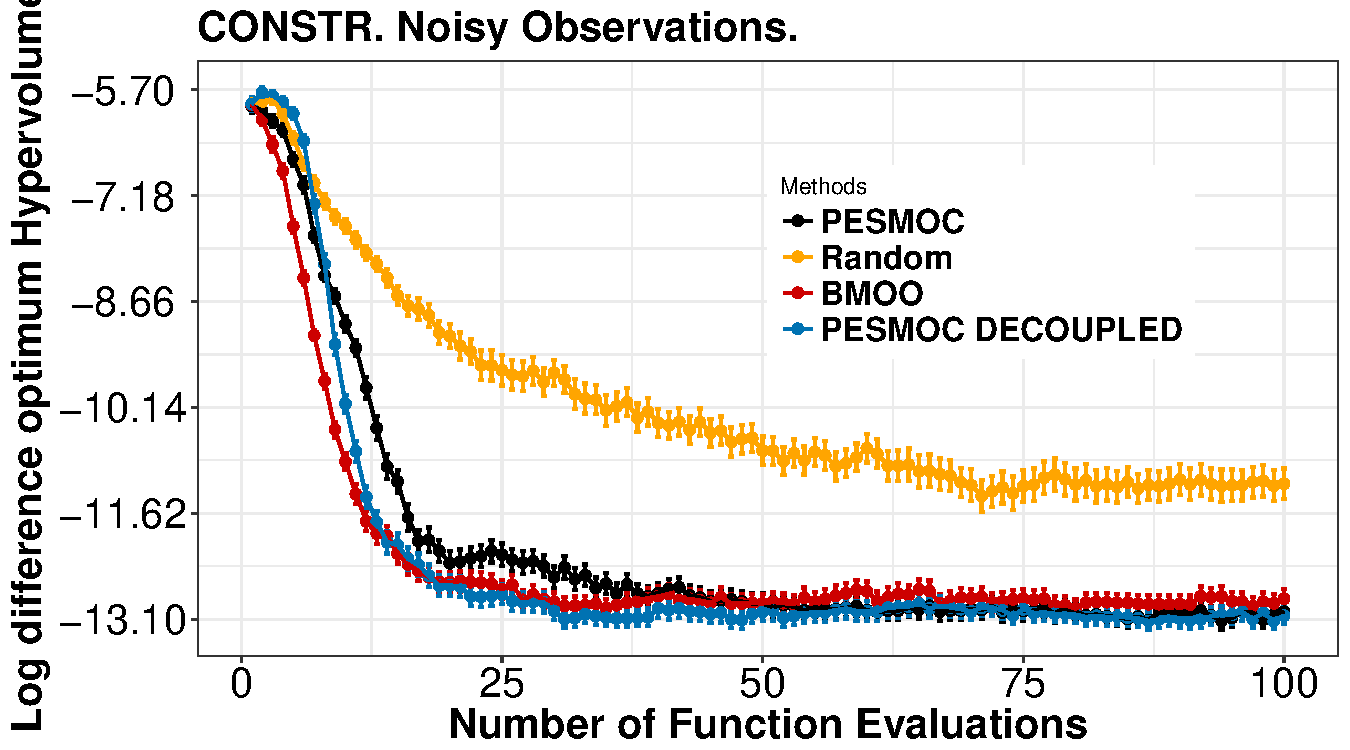
\includegraphics[width=0.475\linewidth]{figures/benchmark/CONSTR_noisy.pdf} \\
		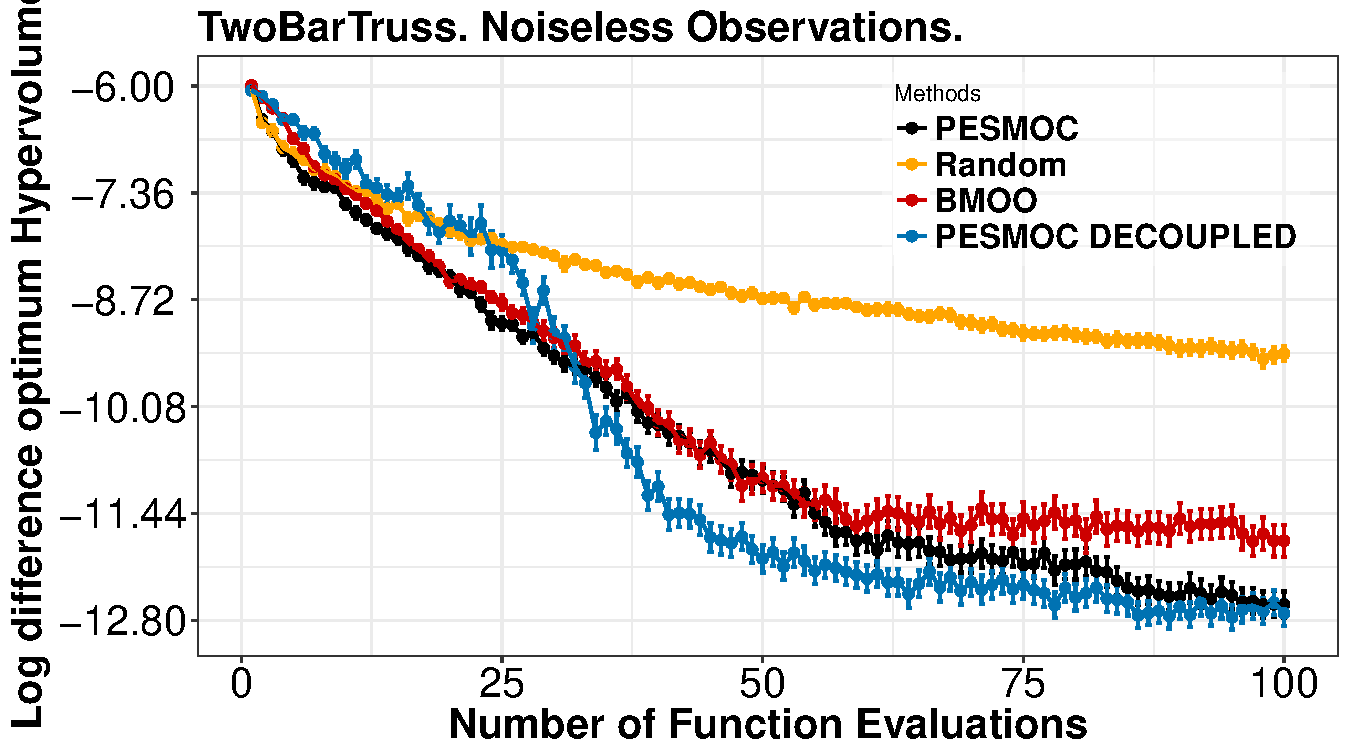
\includegraphics[width=0.475\linewidth]{figures/benchmark/TwoBarTruss.pdf} &
                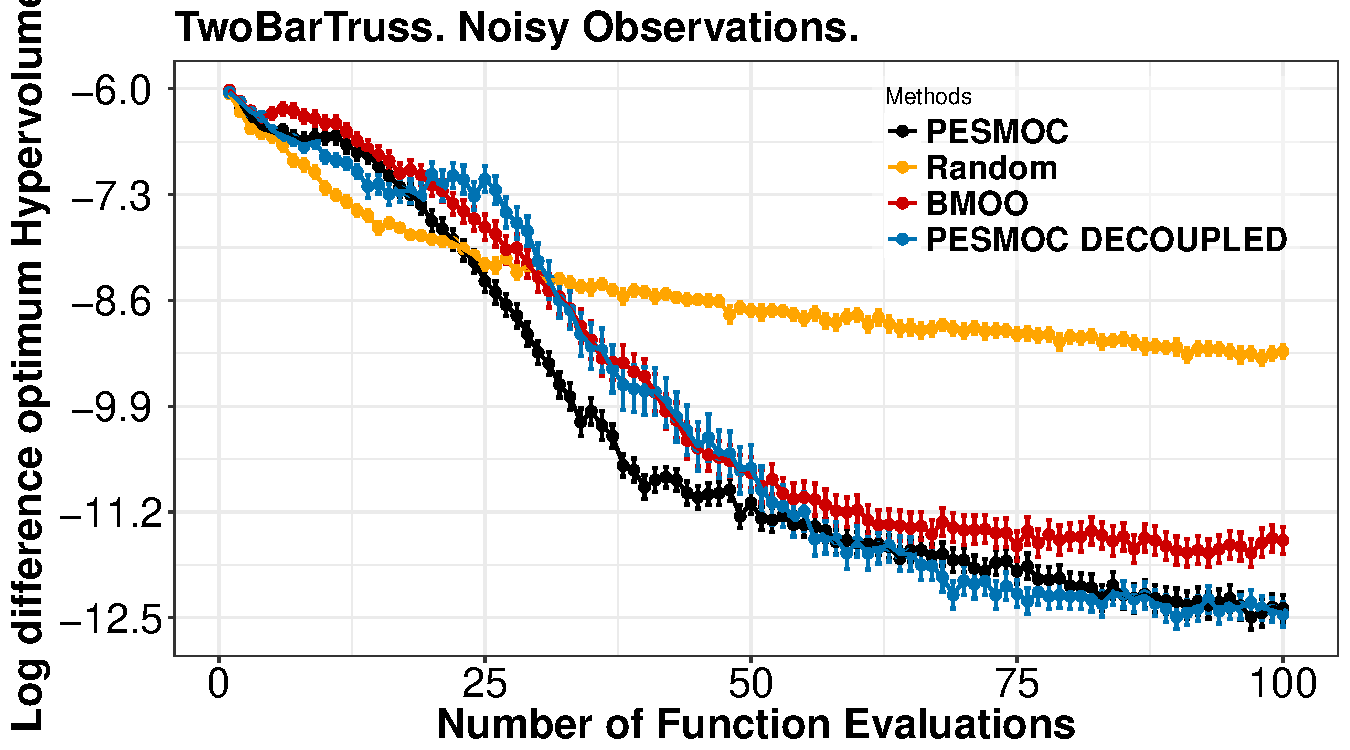
\includegraphics[width=0.475\linewidth]{figures/benchmark/TwoBarTruss_noisy.pdf} \\
		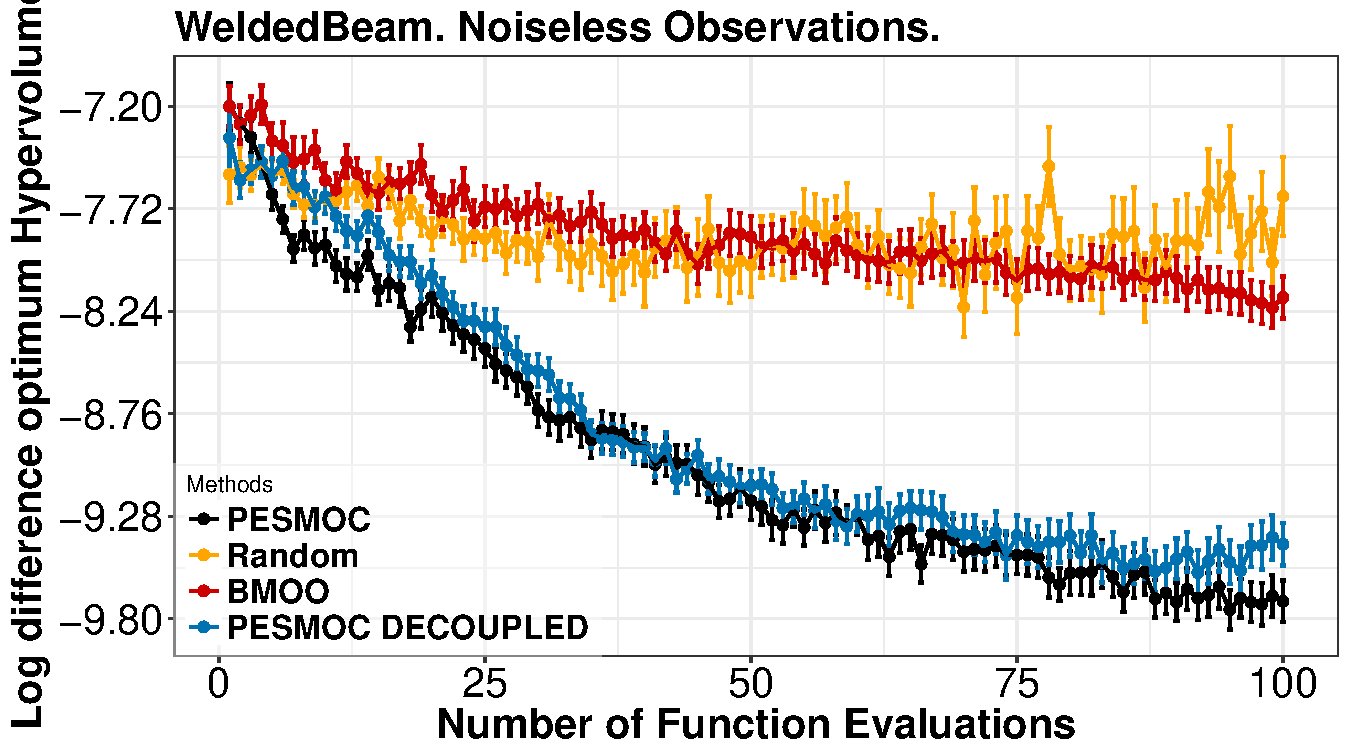
\includegraphics[width=0.475\linewidth]{figures/benchmark/WeldedBeam.pdf} &
                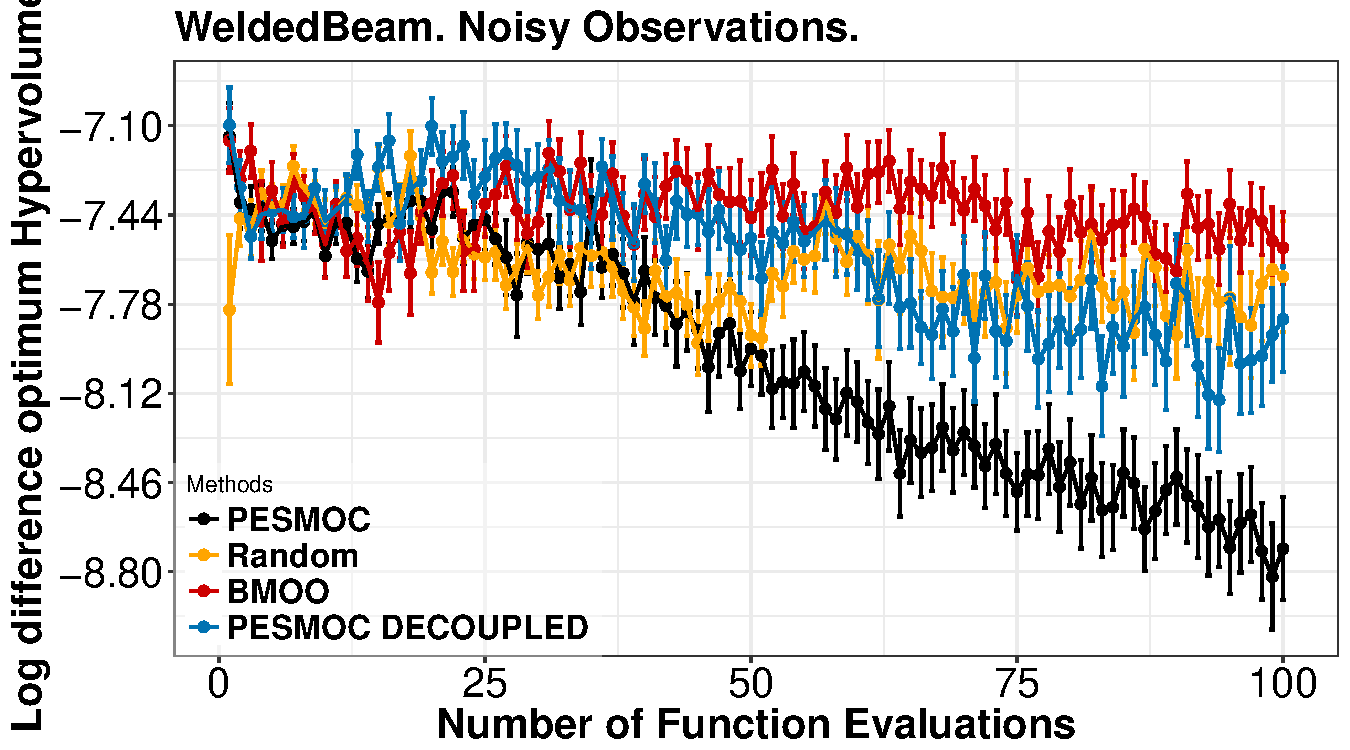
\includegraphics[width=0.475\linewidth]{figures/benchmark/WeldedBeam_noisy.pdf} \\		
		\vspace{-.1cm}
	\end{tabular}
        \caption{Results for CONSTR, TwoBarTruss and WeldedBeam. Noiseless 
		and noisy settings. The plots show the average log difference w.r.t to the optimal hyper-volume.}
        \label{fig:benchmark_results_2}
\end{figure}

%\begin{figure}[htb]
%        \begin{tabular}{cc}
%                \vspace{-.2cm}
%		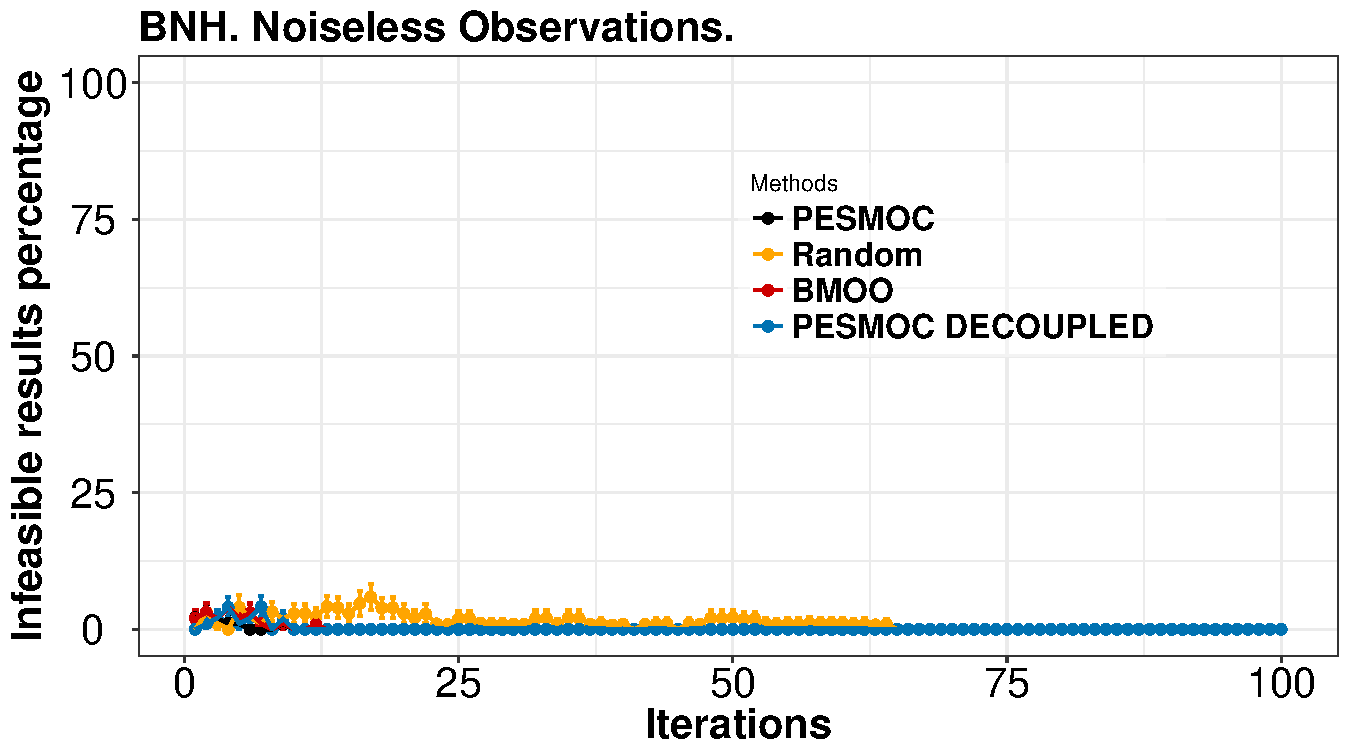
\includegraphics[width=0.475\linewidth]{figures/benchmark/BNH_zeros_noiseless} &
%                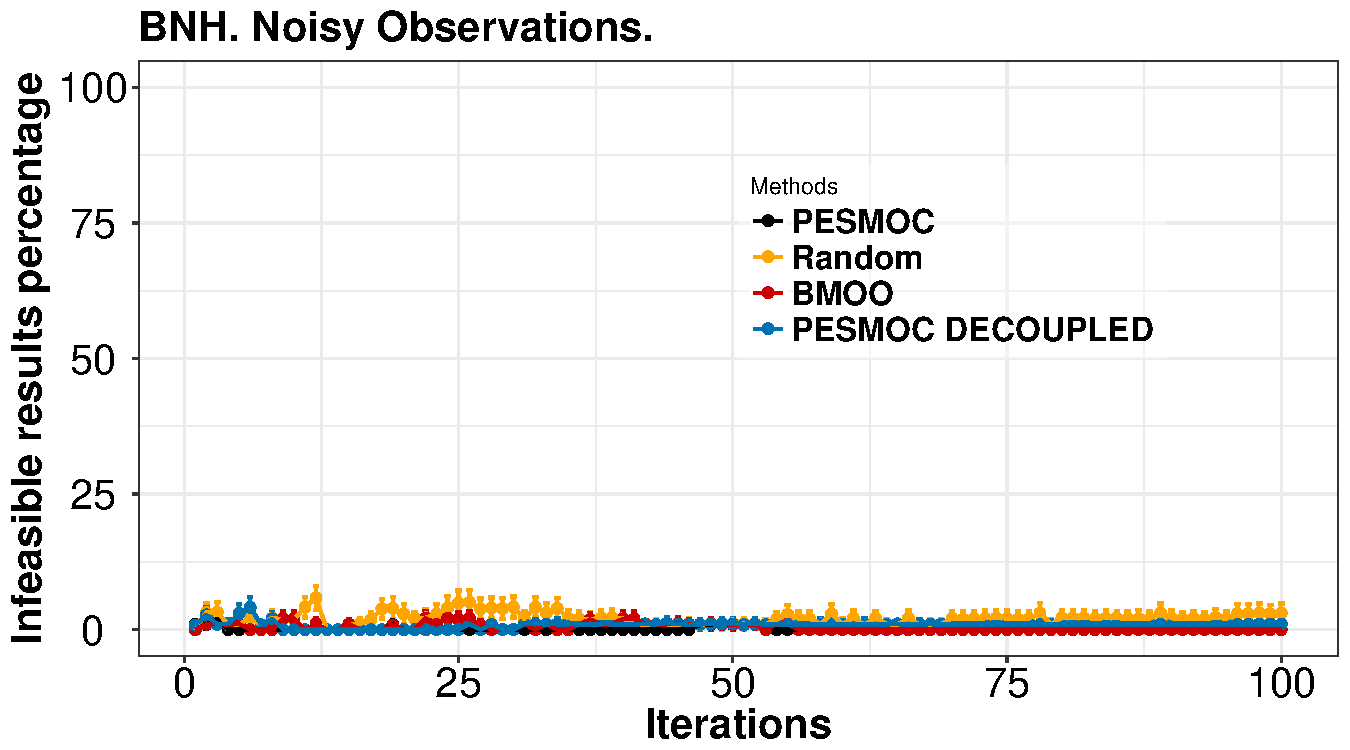
\includegraphics[width=0.475\linewidth]{figures/benchmark/BNH_zeros_noisy} \\
%		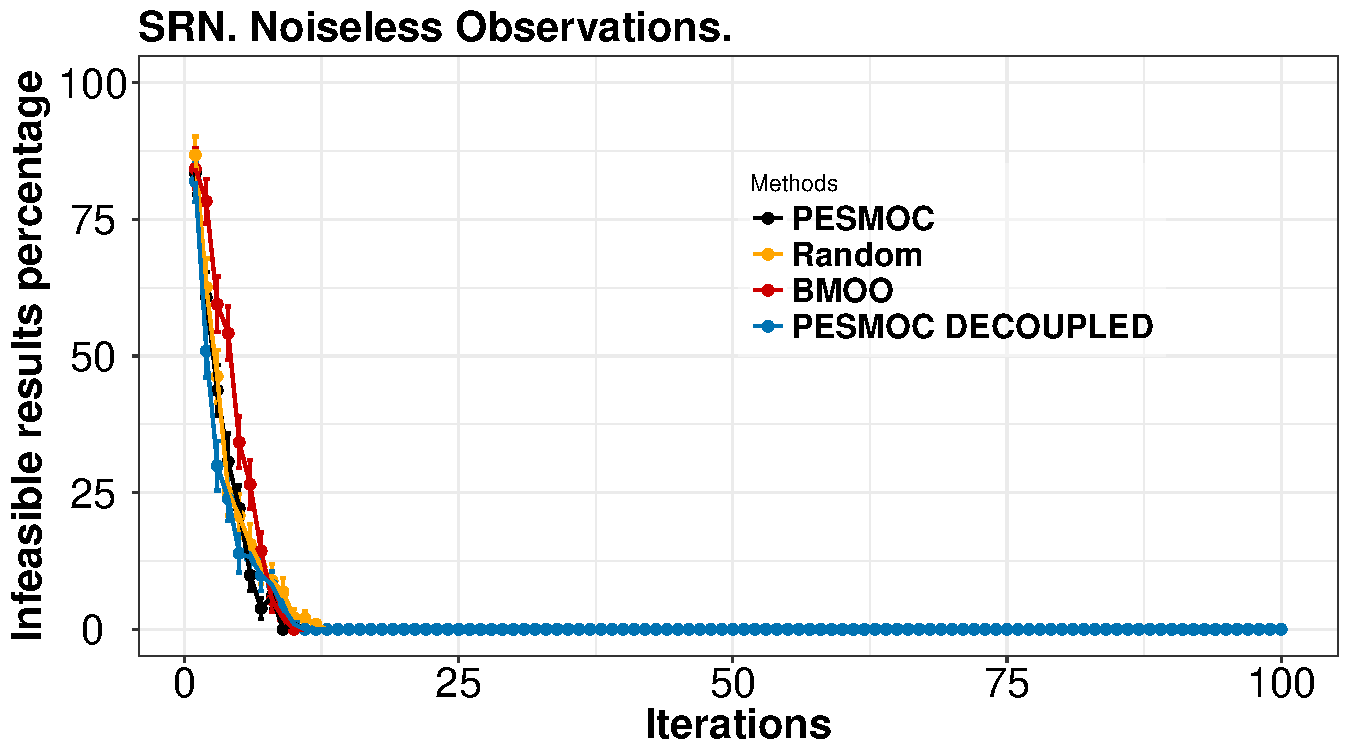
\includegraphics[width=0.475\linewidth]{figures/benchmark/SRN_zeros_noiseless} &
%                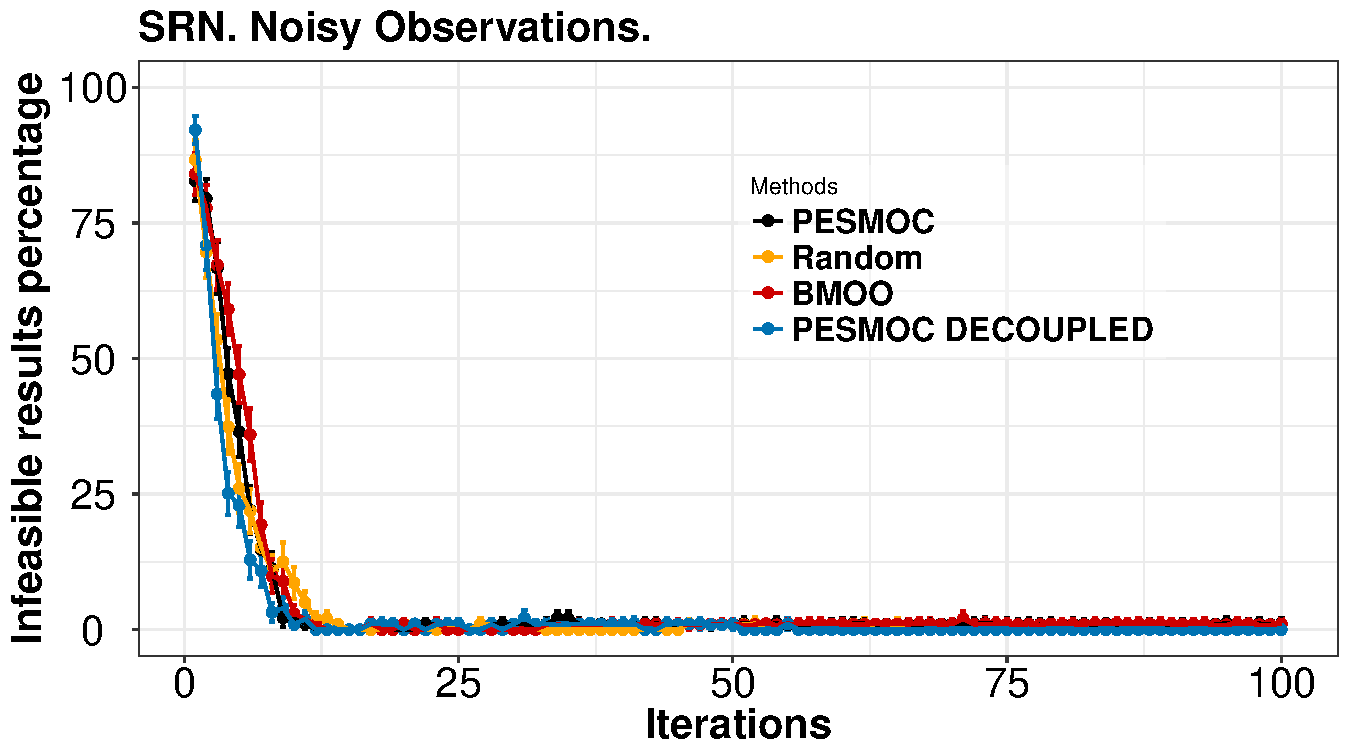
\includegraphics[width=0.475\linewidth]{figures/benchmark/SRN_zeros_noisy} \\
%                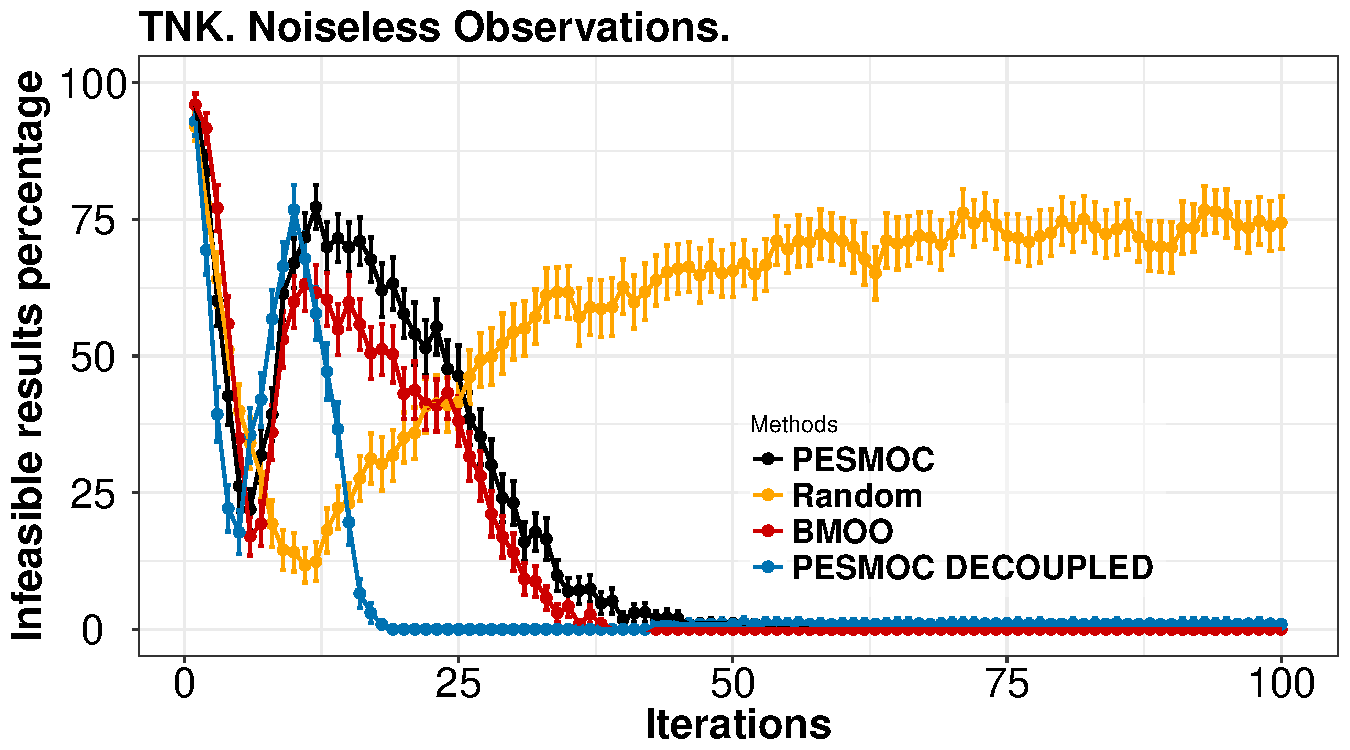
\includegraphics[width=0.475\linewidth]{figures/benchmark/TNK_zeros_noiseless} &
%                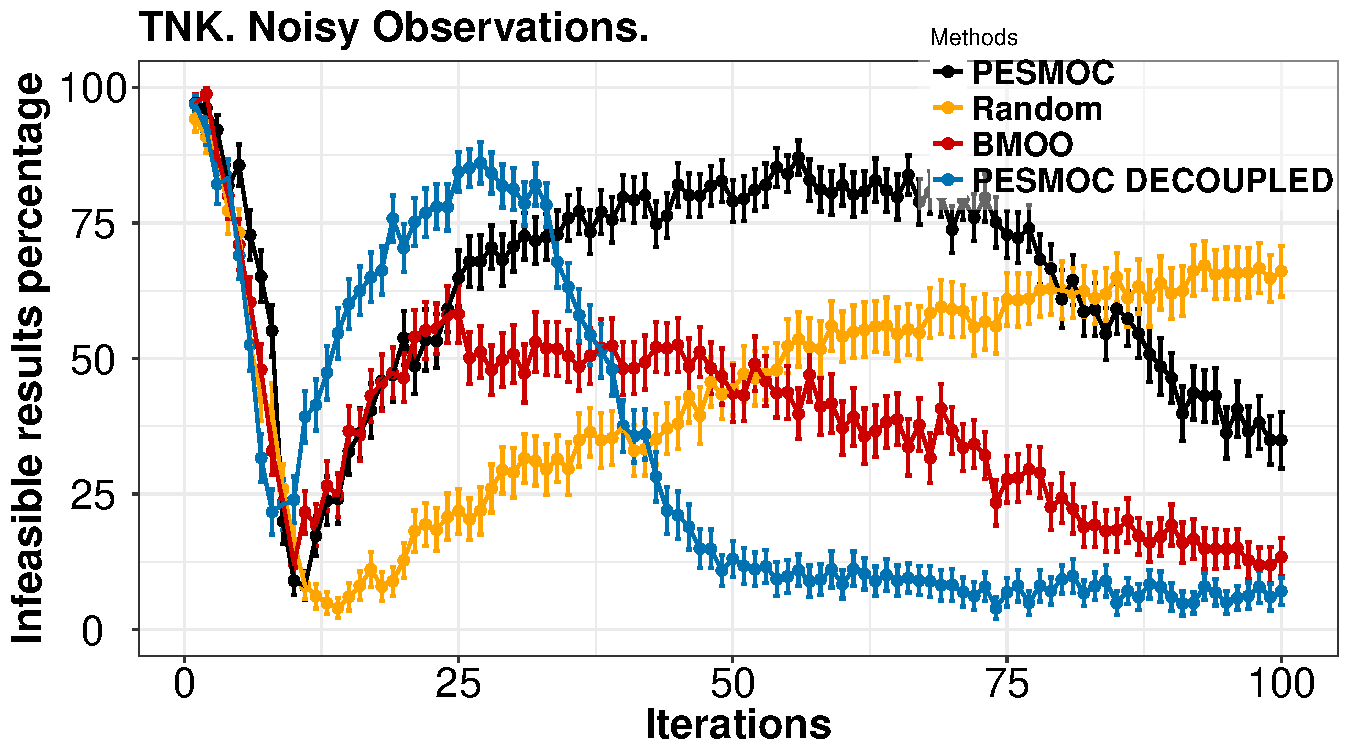
\includegraphics[width=0.475\linewidth]{figures/benchmark/TNK_zeros_noisy} \\
%		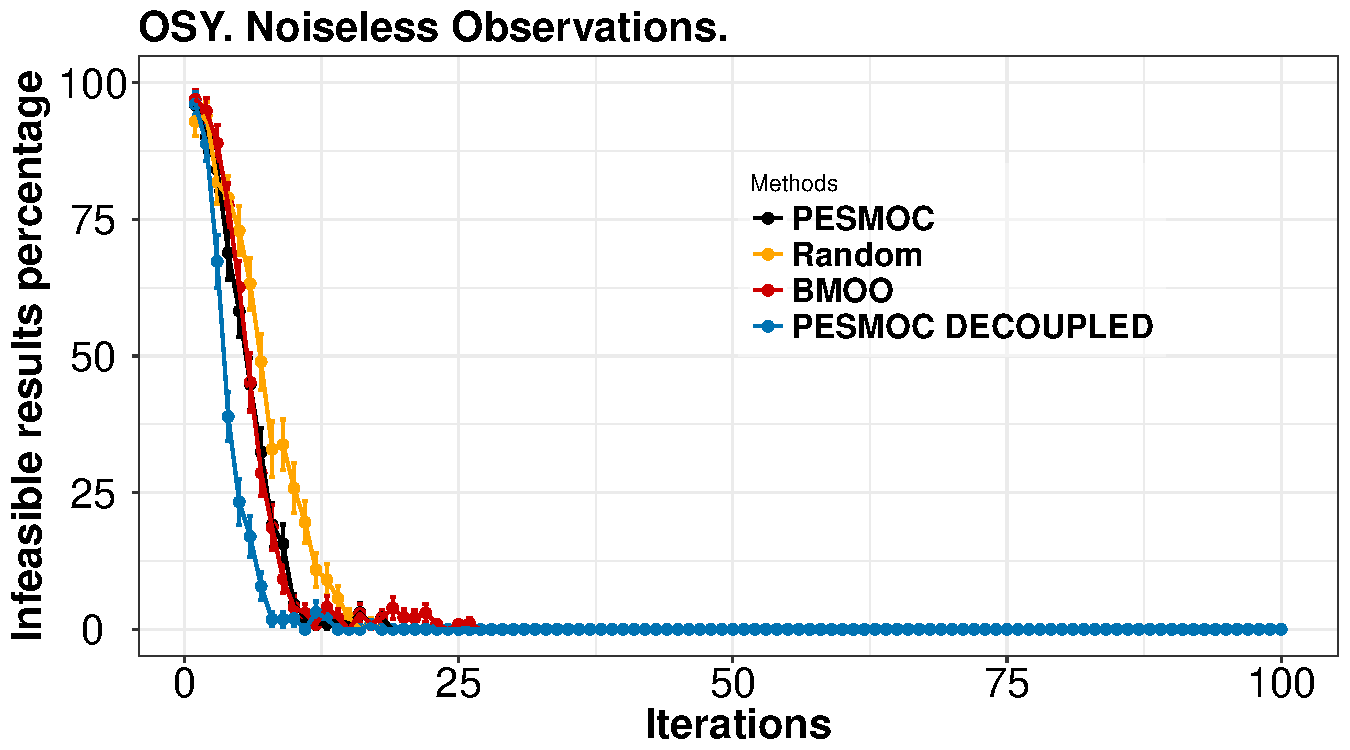
\includegraphics[width=0.475\linewidth]{figures/benchmark/OSY_zeros_noiseless} &
%                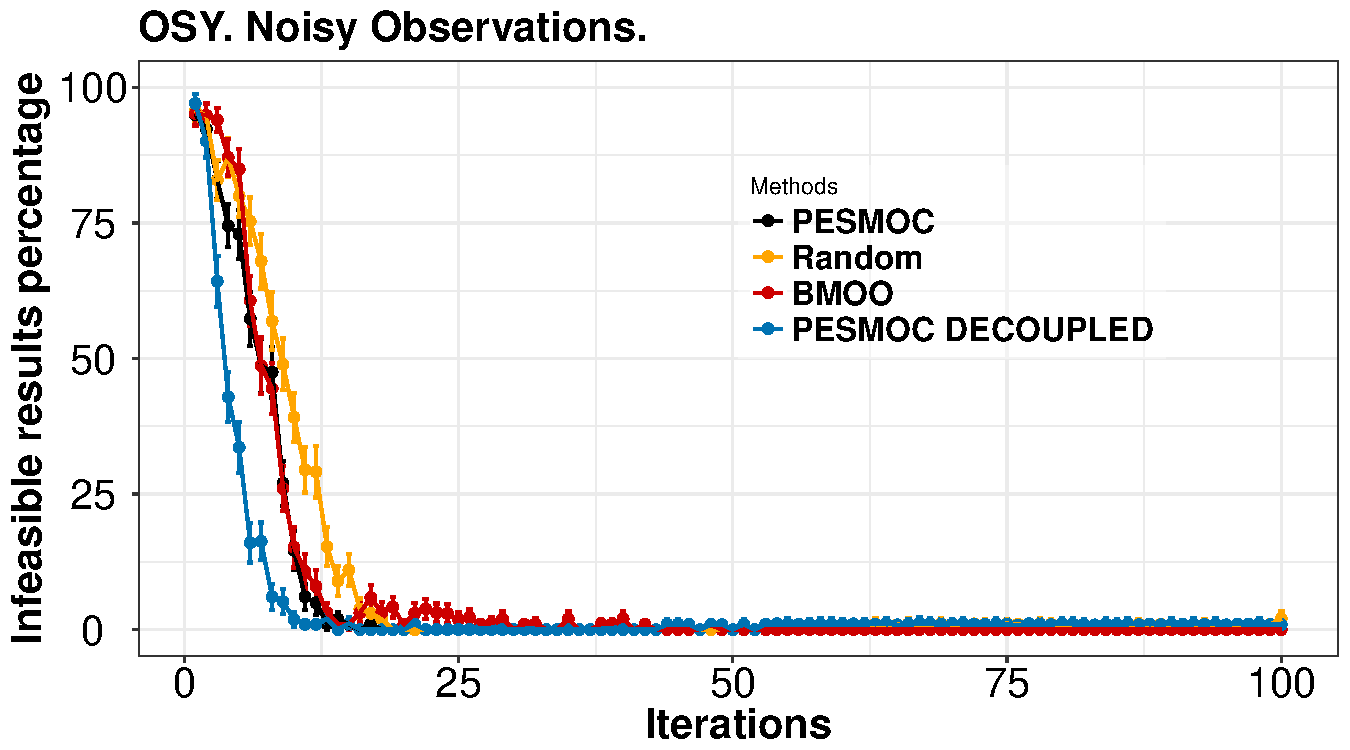
\includegraphics[width=0.475\linewidth]{figures/benchmark/OSY_zeros_noisy} \\
%        \end{tabular}
%        \caption{Infeasible percentage of results in every iteration of experiments BNH, SRN, TNK and OSY.}
%        \label{fig:benchmark_results_3}
%\end{figure}
%
%\begin{figure}[htb]
%        \begin{tabular}{cc}
%                \vspace{-.2cm}
%                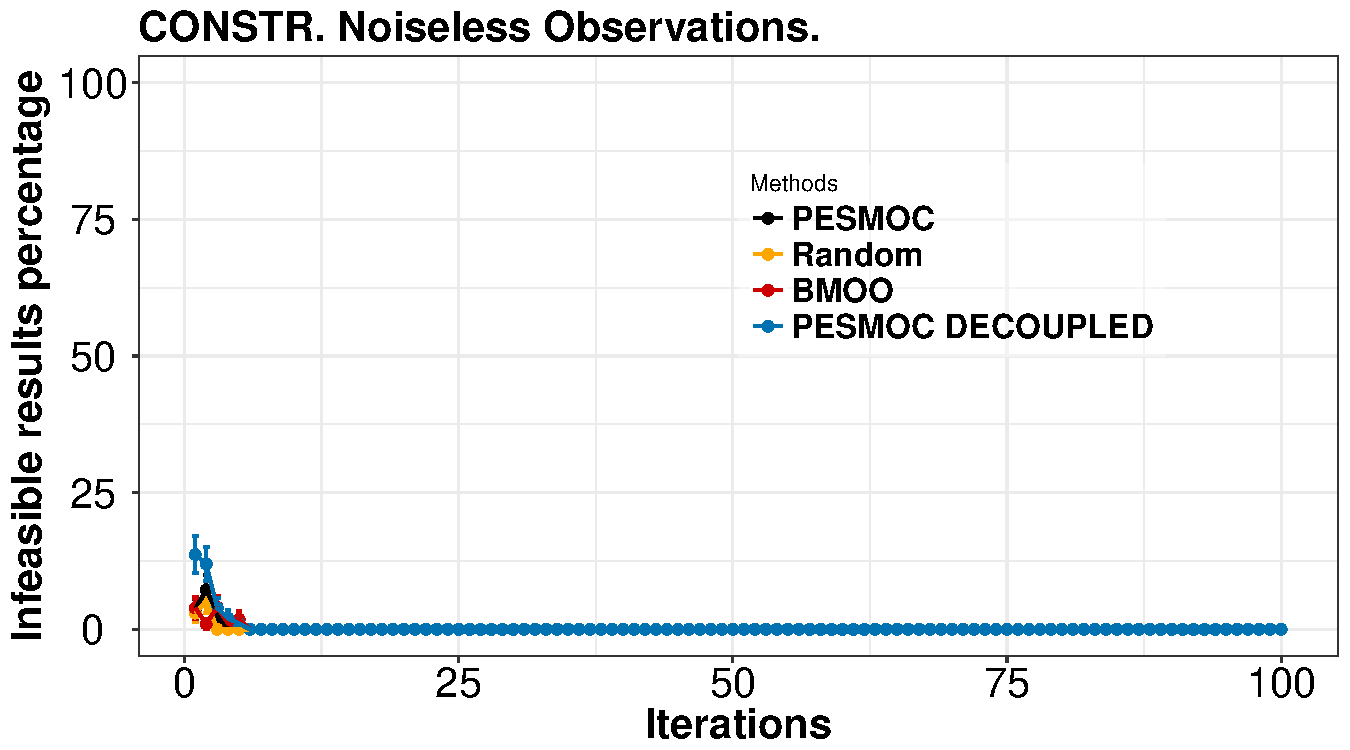
\includegraphics[width=0.475\linewidth]{figures/benchmark/CONSTR_zeros_noiseless} &
%                \includegraphics[width=0.475\linewidth]{figures/benchmark/CONSTR_zeros_noisy} \\
%		\includegraphics[width=0.475\linewidth]{figures/benchmark/TwoBarTruss_zeros_noiseless} &
%                \includegraphics[width=0.475\linewidth]{figures/benchmark/TwoBarTruss_zeros_noisy} \\
%		\includegraphics[width=0.475\linewidth]{figures/benchmark/WeldedBeam_zeros_noiseless} &
%                \includegraphics[width=0.475\linewidth]{figures/benchmark/WeldedBeam_zeros_noisy} \\
%        \end{tabular}
%        \caption{Infeasible percentage of results in every iteration of experiments CONSTR, TwoBarTruss and WeldedBeam.}
%        \label{fig:benchmark_results_5}
%\end{figure}

We observe that, on average, PESMOC in the coupled and decoupled setting, outperforms the other 
methods for multi-objective constrained optimization. BNH is solved pretty fast by all methods, 
but PESMOC, under a decoupled evaluation setting, obtains better results with a smaller number of evaluations.
These differences are also notable in the noisy setting. In this case, PESMOC clearly outperforms BMOO and the 
random search strategy. In the SRN, TNK and OSY problems, results are more or less the same but with bigger 
differences among the methods. BMOO tends to systematically perform worse in the presence of noise. 
Importantly, PESMOC decoupled performs significantly better on TNK. This is because this 
strategy is able to focus on the evaluation of the most difficult black-box functions. 
More precisely, in this problem one of the constraints plays a critical role in the 
identification of the Pareto optimal set and PESMOC decoupled is able to focus on 
its evaluation. This is a clear example of the benefits of a decoupled evaluation setting.
The OSY problem has a higher dimensionality and hence, due to the greedy nature of BMOO that tends 
to explore too much, PESMOC approaches clearly do better. 

The problem CONSTR is very easy to solve so BMOO does a good job on it, leaving PESMOC behind 
but resulting in the same performance as PESMOC decoupled.  TwoBarTruss has the 
same nature as TNK, with the optimum lying in the frontier of the feasible and infeasible space. Again, 
PESMOC decoupled explores massively the constraints, solving the problem and giving better results that 
the other methods with a smaller number of evaluations. In the noise scenario, however, both PESMOC 
approaches tie. The last problem reported is WeldedBeam, where both PESMOC approaches outperform the other methods. 
In the noisy scenario PESMOC under a coupled evaluation setting wins. We believe that model misspecification
and the influence of noise may affect negatively the decoupled approach in certain scenarios. 

\subsection{Finding an Optimal Ensemble of Decision Trees}

We compare the different methods on a practical problem in which the optimal hyper-parameters of an
ensemble of decision trees are optimized. We consider two objectives: the prediction error of the
ensemble and its size. These two objectives are conflictive since smaller ensembles will have in general
higher error rates and the other way around. The ensemble size is related to the storage requirements and
also to the speed of classification, which can play a critical role in real-time prediction systems.
The dataset considered is the German Credit dataset, which is extracted from the UCI repository \citep{Dua2017}. 
This is a binary classification dataset with $1,000$ instances and $20$ attributes. The prediction error is 
measured using a 10-fold-cross validation procedure that is repeated 5 times to reduce the variance of the estimates.
We measure the ensemble size in terms of the logarithm of the sum of the total number of nodes in each of trees of 
the ensemble.

To get ensembles of decision trees with good prediction properties it is essential to enforce diversity among the 
ensemble classifiers \citep{dietterich2000ensemble}. In particular, if all the decision trees of the ensemble are 
equal, there is no expected gain from aggregating their predictions. However, too much diversity in the ensemble 
can also lead to a poor prediction performance. For example, if the predictions made are completely random, 
one cannot obtain improved results by aggregating the individual classifiers. Therefore, we consider 
here several mechanisms to encourage diversity in the ensemble, and let the amount of diversity be specified 
in terms of adjustable parameters.

To build the ensemble we employ decision trees in which the best split at each node corresponds
to the attribute that decreases the most the data impurity among a randomly chosen set 
of attributes (we use the DecisionTree implementation provided in the python package 
scikit-learn), and the number of random attributes is an adjustable parameter. 
This is the approach followed in random forest \citep{breiman2001random}. Each tree 
is trained on a random subset of the training data of a particular size, 
which is another adjustable parameter. This approach is known in the literature
as subbagging \citep{buhlmann2002analyzing}. We consider also an extra method to introduce 
diversity known as class-switching \citep{martinez2005switching}. In class-switching, the labels 
of a random fraction of the training data are changed to a different class. The final ensemble prediction 
is computed by majority voting.

More precisely, the adjustable parameters of the ensemble are: the number of decision trees built 
(between 1 and $1,000$), the number of random chosen attributes considered at each split in the building 
process of each tree (between 1 and 20), the minimum number of samples required to split a node (between 2 and
200), the fraction of randomly selected training data used to build each tree (between 0.5 and 1.0), 
and the fraction of training instances whose labels are changed after the sub-sampling process 
(between $0.0$ and $0.7$).

A problem of classification ensembles is that computing predictions can take much longer than using a single 
classifier. The reason for this is that one has to query all the ensemble classifiers about the class 
label of each test instance. A potential way of accelerating predictions is to use a dynamic ensemble pruning 
technique \citep{hernandez2009statistical}. Assume that for a test instance we have queried only 
a fraction of the ensemble classifiers. It is possible to estimate the probability  that 
the majority vote decision of the ensemble is not changed by the votes of the remaining classifiers. If 
this probability exceeds a particular threshold (\emph{e.g.}, 99\%), the querying process can be early stopped 
and the current majority class can be returned as the final ensemble prediction. Therefore, we introduce as 
a constraint of the optimization problem, that the average speed up factor of the classification process 
given by the previous dynamic ensemble pruning technique is at least 25\%. 
We have carefully chosen this value to guarantee that the constraint is active at the optimal solution. 
In practice, the methods compared rarely provide infeasible solutions. If this is the case, we simply ignore those recommendations.

Note that the setting described is suited for the decoupled version of PESMOC since both objectives 
and the constraint can be evaluated separately. In particular, the total number of nodes is estimated 
by building only once the ensemble without leaving any data aside for validation, as opposed to the
cross-validation approach used to estimate the ensemble error, which requires to build several
ensembles on subsets of the data, to then estimate the prediction error on the data left out for
validation. Similarly, evaluating the constraint involves building a lookup table whose entries indicate, for 
each different number of classifiers queried so far, how many votes of the most common class are needed to 
early stop the prediction process. This table is expensive to build and is different for each ensemble size.
See \citep{hernandez2009statistical} for further details.

We report in Figure \ref{fig:ensemble_results} the results obtained for each method 
after $100$ and $200$ evaluations of the corresponding black-box functions. This figure shows the 
average Pareto front obtained by each method across the 100 different repetitions of the experiments.
The Pareto front is simply given by the objective values associated to the recommendation made by each
method. In general, and assuming minimization, the higher the volume of points that is above this set
of points in the objective values space the better the performance of a method, as estimated by the 
hyper-volume metric. We observe that PESMOC outperforms BMOO and the random search strategy. Furthermore, 
PESMOC decoupled obtains better results that PESMOC. More precisely, PESMOC and PESMOC decoupled find 
better solutions in the sense that the ensembles obtained have a lower size and a smaller prediction error.
Last, we note that BMOO is able to find the ensembles of the smallest size, but with higher levels of 
error, in a smaller number of evaluations.

We also show in Table \ref{table:hyper_ensemble} the average hyper volume of the solutions provided by each 
method. In general, a higher hyper-volume implies that the method gives better results. The values obtained agree with 
the previous figure. Namely, PESMOC decoupled outperforms the other methods, followed closely by PESMOC in a 
coupled setting, BMOO and the random search strategy. After 200 evaluations the differences in the hyper-volume 
between PESMOC decoupled and the other methods become bigger. This is probably a consequence of 
PESMOC decoupled performing more evaluations of the most complicated black-box function.

% DHL: TODO check if the number of evaluations is 200 or 300
% EGM: The plot is generated for 200 evaluations, the name of the file is an errata.

\begin{figure}[H]
\begin{center}
        \begin{tabular}{cc}
                \vspace{-.2cm}
                \includegraphics[width=0.75\linewidth]{figures/real/100_ensemble.pdf} \\ \\
                \includegraphics[width=0.75\linewidth]{figures/real/200_ensemble.pdf} \\
                \vspace{-.1cm}
        \end{tabular}
        \caption{Results of each method on the problem of finding an optimal ensemble of classification trees.
		The Pareto frontier is shown for each method. The volume of points above the frontier 
		(hyper-volume) represents the quality of the solution. A wider volume is always better.}
        \label{fig:ensemble_results}
\end{center}
\end{figure}

\begin{table}[htb]
\small
\centering
\caption{Average hyper-volume of each method on the task of finding an optimal classification 
	ensemble. Larger hyper-volumes means better quality. PESMOC c. means PESMOC coupled and PESMOC d. means 
PESMOC decoupled.}
\begin{tabular}{ c c c c c}
 \hline
\textbf{\# Eval.} & \textbf{PESMOC c.} & \textbf{PESMOC d.} & \textbf{BMOO} & \textbf{Random} \\
\hline
100 & $ 0.309  \pm  0.001 $ & $\mathbf{ 0.311 \pm  0.002 }$ & $ 0.293 \pm  0.001$ & $ 0.265 \pm  0.002 $ \\
\hline
200 & $ 0.325 \pm  0.001 $ & $\mathbf{ 0.338 \pm  0.001 }$ & $ 0.309 \pm  0.001 $ & $ 0.279 \pm  0.001$ \\
\hline
\end{tabular}
\label{table:hyper_ensemble}
\end{table}

In the problem described, we expect the prediction error to be the black-box function with the most important 
role in solving the optimization problem. Probably, it is more difficult to model than the the ensemble 
size or the speed-up factor due to the dynamic pruning technique. To check this hypothesis we record for 
PESMOC decoupled the number of times that each black-box function is evaluated. The average results obtained are 
shown in Figure \ref{fig:decoupled_ensemble}. 
This figure shows, for each iteration of the optimization process, the average number of evaluations of each
black-box function performed by PESMOC decoupled. 
We can see that the previous hypothesis is validated by the plot. 
Namely, the prediction error is evaluated more frequently than the other black-box functions. This also explains 
the better results obtained by PESMOC decoupled. In particular, this technique is able to focus on the evaluation of
the most important black-box function. Of course, the prediction error takes more time to evaluate than the 
other black-box functions, so PESMOC decoupled also takes a bit more time than the other techniques. In any case, 
this result illustrates the potential benefits of a decoupled evaluation strategy, which chooses not only at which
point to perform the evaluation, but also which black-box function should be evaluated each time.

\begin{figure*}[htb]
\begin{center}
        \begin{tabular}{cc}
                \vspace{-.2cm}
                \includegraphics[width=0.75\linewidth]{figures/real/plot_ensemble_counter.pdf} \\ \\
                \vspace{-.1cm}
        \end{tabular}
        \caption{Evaluations of each black-box function made by PESMOC decoupled in the problem of finding an optimal
	ensemble of decision tree classifiers. The error objective is black-box function chosen most frequently for evaluation.} 
        \label{fig:decoupled_ensemble}
\end{center}
\end{figure*}


\subsection{Finding an Optimal Deep Neural Network}

In this section we evaluate the performance of the different methods on the task of finding an optimal
deep neural network on the MNIST dataset \citep{lecun2010mnist}. This dataset contains a training set 
of 60,000 instances. The objectives that we consider for this problem include minimizing the prediction error 
of the neural network on a validation dataset of 10,000 instances (extracted from the original training set) 
and minimizing the time that such a neural network will take for making predictions on such a set. Note that these 
are conflictive objectives in the sense that most probably minimizing the prediction error on the validation 
set will require bigger neural networks with a larger number of hidden units 
and layers. Of course, these neural networks will require longer prediction times. Conversely, the minimization of 
the prediction time will probably involve using neural networks of smaller size whose prediction performance will be worse.

Besides this, we also consider that we may be interested in codifying such a neural network into a chip. This can be 
interesting for example if we would like to use that neural network in an electronic device such as an smart-phone.
Motivated by this scenario we propose to constrain the optimization problem in such a way that the area of the
resulting deep neural network, after being codified into a chip, is below one squared millimeter. 
We have carefully chosen this value to guarantee that the constraint is active at the optimal solution. 
To measure this area we use the  hardware simulator Aladdin \citep{shao2014aladdin}, which given 
a computer program describing the operations carried out 
by the deep neural network, outputs an estimate of the area of a chip implementing those 
operations.  

In practice, the methods compared rarely provide infeasible solutions. If this is the case, we simply ignore those 
recommendations. To train the deep neural network we use the Keras library \citep{chollet2015keras}. 
Prediction time is measured on the validation set of $10,000$ training instances.  
The prediction time is normalized by the smallest possible prediction time, which corresponds to 
a neural network of a single layer with $5$ hidden units. 

Importantly, the different black-box functions involved in the optimization problem just described can be 
evaluated separately in a decoupled way. The reason for this is that the prediction time and the chip 
area does not need specific values for the neural network weights and biases. These can simply be 
initialized randomly. These two black-box functions only depend on the particular architecture of the 
neural network (the number of layers and the number of hidden units on each layer). Therefore, the problem described 
is adequate for PESMOC decoupled. The specific steps involved in measuring the different black-boxes are 
displayed in Figure \ref{fig:arch_alad}.

% DHL TODO update this diagram to show the actual information flow
% EGM Done.

\begin{figure}[htb]
\begin{center}
        \begin{tabular}{cc}
                \vspace{-.2cm}
                \includegraphics[width=0.99\linewidth]{figures/real/diagrams/architecture_real_hard_exp.pdf} \\ \\
                \vspace{-.1cm}
        \end{tabular}
        \caption{Diagram showing the architecture of systems that we have used for the deep neural network experiments.
		The different steps involved in the evaluation of each black-box function are displayed here.}
        \label{fig:arch_alad}
\end{center}
\end{figure}

The input parameters that we consider for optimization in this problem are: 
The logarithm of the $\ell_1$  and $\ell_2$ weight regularizers; 
the dropout probability; the logarithm of the initial learning 
rate; the number of hidden units per layer; and the number of hidden layers. We have also 
considered two variables that have an impact in the hardware implementation 
of the neural network. Namely, the logarithm (in base 2) of the array partition factor 
and the loop unrolling factor. See \citep{shao2014aladdin} for further details. 
A summary of the parameters considered, their potential values, and their impact in each 
black-box function (prediction error, time and chip area) is displayed in Table \ref{table:aladdin}.

\begin{table}[htb]
\centering
\caption{Parameter space of the deep neural network experiments. PE = Prediction error. T = Time. CA = Chip area.}
\begin{tabular}{lcccc}
 \hline
\textbf{Parameter} & \textbf{Min} & \textbf{Max} & \textbf{Step} & \textbf{Black-box} \\
 \hline
Hidden Layers & 1& 3& 1& PE/T/CA\\
Neurons per Layer & 5& 300& 1& PE/T/CA\\
Learning rate & $e^{-20}$& 1& $\epsilon$ & PE\\
Dropout rate & 0& 0.9& $\epsilon$ & PE\\	
$\ell_1$ penalty & $e^{-20}$& 1& $\epsilon$ & PE\\
$\ell_2$ penalty & $e^{-20}$& 1& $\epsilon$ & PE\\
\hline
Memory partition & 1& 32& $2^{x}$& CA\\
Loop unrolling & 1& 32& $2^{x}$& CA\\
\hline
\end{tabular}
\label{table:aladdin}
\end{table}

In these experiments we evaluated the performance of each method after $50$ and $100$ evaluations of the black-boxes.
Furthermore, the training of the deep neural networks is carried out using ADAM with the default parameter values 
\citep{kingma2014adam}. The loss function is the  categorical cross-entropy. The last layer of the 
neural network contains 10 units and a soft-max activation function. All other layers use 
Re-Lu as the activation function. Finally, each neural network is trained during a total of 
$150$ epochs using mini-batches of size $4,000$ instances.

The average results obtained across 100 repetitions of the experiments can be shown in 
Figure \ref{fig:nnet_results} after $50$ and $100$ evaluations of the black-boxes. This 
figure shows the average Pareto frontier obtained by each method. As in the previous experiments 
PESMOC decoupled outperforms the others methods. PESMOC is the second best method, giving 
solutions with a best trade-off between prediction error and time ratio (prediction time normalized with respect
to the smallest possible prediction time), under the constraint that the chip area
is below the specified value. BMOO also gives better results than the random search strategy which 
is the worst performing method. These experiments show strong empirical evidence supporting
that PESMOC is a competitive strategy for constrained multi-objective optimization. 
We also provide the average hyper-volume of the solutions found by each method after $50$ and $100$ evaluations 
of the black-boxes. These results are displayed in Table \ref{table:aladdin_hypervolume}. We observe that PESMOC 
decoupled outperforms the rest of the methods. This strategy finds solutions that, on average, have 
a significantly higher hyper-volume than any of the other methods. Furthermore, PESMOC is 
able to find solutions that are slightly better than those obtained by BMOO.

% DHL TODO Update the y axis in the figures. It should be Time Ratio
% EGM Done.

\begin{figure}[H]
\begin{center}
        \begin{tabular}{cc}
                \vspace{-.2cm}
                \includegraphics[width=0.75\linewidth]{figures/real/50_nnet.pdf} \\ \\
                \includegraphics[width=0.75\linewidth]{figures/real/100_nnet.pdf} \\
                \vspace{-.1cm}
        \end{tabular}
        \caption{Results of each method on the problem of finding an optimal neural network on the MNIST dataset.
		The Pareto frontier is shown for each method. The volume of points above the frontier 
		(hyper-volume) represents the quality of the solution. A wider volume is always better.}
        \label{fig:nnet_results}
\end{center}
\end{figure}

% DHL TODO check standard deviations. They look too small.
% EGM Validated. 

\begin{table}
\centering
\caption{Average hyper-volume of each method on the task of finding an optimal neural network on the MNIST dataset.
	Larger hyper-volumes means better quality. PESMOC c. means PESMOC coupled and PESMOC d. means 
PESMOC decoupled.}
\begin{tabular}{lcccc}
 \hline
\textbf{\# Eval.} & \textbf{PESMOC c.} & \textbf{PESMOC d.} & \textbf{BMOO} & \textbf{Random} \\
 \hline
50 & $ 47.230  \pm  0.079 $ & $\mathbf{ 47.608  \pm  0.056 }$ & $ 46.104 \pm 0.267 $ & $ 44.886  \pm  0.135 $ \\
\hline
100 & $ 47.621  \pm  0.054 $ & $\mathbf{ 48.069  \pm  0.039 }$ & $ 47.304  \pm  0.083 $ & $ 45.714  \pm  0.093 $ \\
\hline
\end{tabular}
\label{table:aladdin_hypervolume}
\end{table}

We also analyze in these experiments which black-box function is evaluated more frequently by PESMOC decoupled.
For this, we record the number of evaluations of each black-box made by this strategy as a function of the 
total evaluations made. The average results obtained across the 100 repetitions of the experiments are shown 
in Figure \ref{fig:nnet_counter}. We observe that  PESMOC decoupled tends to evaluate a significantly higher
number of times the prediction error of the neural network. This also explains the better results obtained
by this strategy which is able to focus on the evaluation of the black-box function that is most difficult to
model or that plays a critical role in the optimization problem. Of course, the prediction error takes more 
time to evaluate than the other black-box functions, so PESMOC decoupled also takes a bit more time than the 
other techniques in this problem. In any case, this result illustrates again the potential benefits of a 
decoupled evaluation strategy, which can be used to choose in an intelligent way which black-box function 
should be evaluated next at each iteration of the optimization process.

\begin{figure}[htb]
\begin{center}
        \begin{tabular}{cc}
                \vspace{-.2cm}
                \includegraphics[width=0.75\linewidth]{figures/real/plot_rrnn_counter.pdf} \\ \\
                \vspace{-.1cm}
        \end{tabular}
        \caption{Evaluations of each black-box function made by PESMOC decoupled in the problem of finding an optimal
	neural network on the MNIST dataset. The error is black-box function that is chosen most frequently for evaluation 
	by PESMOC decoupled.} 
        \label{fig:nnet_counter}
\end{center}
\end{figure}

\section{Conclusions}
\label{sec:conclusions}

We have described an information-based approach that can
be used to address a wide range of Bayesian optimization problems,
including multiple objectives and several constraints.
Motivated by the lack of methods that are available to solve these
problems with an adequate exploration-exploitation balance,
PESMOC has been presented. At each iteration, PESMOC
evaluates the objective functions and the constraints at an input
location that is expected to reduce the entropy of the posterior
distribution of the Pareto set in the feasible space the most. The 
computation of the expected reduction of the entropy of such a random variable is
intractable. Nevertheless,  we have described how the required computations can 
be approximated using expectation propagation \citep{minka2001expectation}.

Importantly, in the proposed approach the acquisition function can be expressed
as a sum of a different acquisition per black-box function (objective or constraint).
This means that PESMOC allows for a decoupled evaluation setting. In this scenario one is 
not only interested in finding which is the next point at which the black-boxes should
be evaluated, but also in finding what black-box function or subset of these should be evaluated 
next. For this, one simply has to optimize the individual acquisition functions and compare their
corresponding values. Other related methods from the literature do not allow for such a setting
since the utility function they are based on (the improvement of the hyper-volume metric) requires 
the evaluation of all the black-box functions.

We have illustrated in a wide range of experiments, including synthetic, benchmark and real-world problems
the benefits of PESMOC. Furthermore, we have compared results in these experiments with
a state-of-the-art method for constrained multi-objective Bayesian optimization, BMOO \citep{feliot2015bayesian},
which is based on the expected improvement of the hyper-volume, and with a baseline method that explores the input 
space uniformly at random. These experiments show that PESMOC is able to obtain better results in 
terms of the hyper-volume of the recommendations made. More precisely, it provides estimates of the Pareto 
set in the feasible space that are more accurate with a smaller number of evaluations. Furthermore, PESMOC in a 
decoupled setting is able to provide significantly better results in several of these problems. This is very 
useful in practical situations in which the objectives and the constraints are very expensive to evaluate.

\section*{Acknowledgments}

{\small
The authors acknowledge the use of the facilities of Centro de Computaci\'on Cient\'ifica (CCC) at 
Universidad Aut\'onoma de Madrid, and financial support from the Spanish Plan Nacional I+D+i, 
Grants TIN2016-76406-P and TEC2016-81900-REDT, and from Comunidad de Madrid, Grant S2013/ICE-2845 CASI-CAM-CM. 
}

\DIFdelbegin %DIFDELCMD < \bibliography{bibliography}
%DIFDELCMD < %%%
\DIFdelend \DIFaddbegin \bibliography{bibliography}
\DIFaddend 

\bibliographystyle{plain}

\end{document}
